\documentclass[]{tufte-book}

% ams
\usepackage{amssymb,amsmath}

\usepackage{ifxetex,ifluatex}
\usepackage{fixltx2e} % provides \textsubscript
\ifnum 0\ifxetex 1\fi\ifluatex 1\fi=0 % if pdftex
  \usepackage[T1]{fontenc}
  \usepackage[utf8]{inputenc}
\else % if luatex or xelatex
  \makeatletter
  \@ifpackageloaded{fontspec}{}{\usepackage{fontspec}}
  \makeatother
  \defaultfontfeatures{Ligatures=TeX,Scale=MatchLowercase}
  \makeatletter
  \@ifpackageloaded{soul}{
     \renewcommand\allcapsspacing[1]{{\addfontfeature{LetterSpace=15}#1}}
     \renewcommand\smallcapsspacing[1]{{\addfontfeature{LetterSpace=10}#1}}
   }{}
  \makeatother
\fi

% graphix
\usepackage{graphicx}
\setkeys{Gin}{width=\linewidth,totalheight=\textheight,keepaspectratio}

% booktabs
\usepackage{booktabs}

% url
\usepackage{url}

% hyperref
\usepackage{hyperref}

% units.
\usepackage{units}


\setcounter{secnumdepth}{2}

% citations
\usepackage{natbib}
\bibliographystyle{apalike}
%\renewcommand{\bibsection}{\chapter*{References}}

% pandoc syntax highlighting
\usepackage{color}
\usepackage{fancyvrb}
\newcommand{\VerbBar}{|}
\newcommand{\VERB}{\Verb[commandchars=\\\{\}]}
\DefineVerbatimEnvironment{Highlighting}{Verbatim}{commandchars=\\\{\}}
% Add ',fontsize=\small' for more characters per line
\usepackage{framed}
\definecolor{shadecolor}{RGB}{248,248,248}
\newenvironment{Shaded}{\begin{snugshade}}{\end{snugshade}}
\newcommand{\KeywordTok}[1]{\textcolor[rgb]{0.13,0.29,0.53}{\textbf{{#1}}}}
\newcommand{\DataTypeTok}[1]{\textcolor[rgb]{0.13,0.29,0.53}{{#1}}}
\newcommand{\DecValTok}[1]{\textcolor[rgb]{0.00,0.00,0.81}{{#1}}}
\newcommand{\BaseNTok}[1]{\textcolor[rgb]{0.00,0.00,0.81}{{#1}}}
\newcommand{\FloatTok}[1]{\textcolor[rgb]{0.00,0.00,0.81}{{#1}}}
\newcommand{\ConstantTok}[1]{\textcolor[rgb]{0.00,0.00,0.00}{{#1}}}
\newcommand{\CharTok}[1]{\textcolor[rgb]{0.31,0.60,0.02}{{#1}}}
\newcommand{\SpecialCharTok}[1]{\textcolor[rgb]{0.00,0.00,0.00}{{#1}}}
\newcommand{\StringTok}[1]{\textcolor[rgb]{0.31,0.60,0.02}{{#1}}}
\newcommand{\VerbatimStringTok}[1]{\textcolor[rgb]{0.31,0.60,0.02}{{#1}}}
\newcommand{\SpecialStringTok}[1]{\textcolor[rgb]{0.31,0.60,0.02}{{#1}}}
\newcommand{\ImportTok}[1]{{#1}}
\newcommand{\CommentTok}[1]{\textcolor[rgb]{0.56,0.35,0.01}{\textit{{#1}}}}
\newcommand{\DocumentationTok}[1]{\textcolor[rgb]{0.56,0.35,0.01}{\textbf{\textit{{#1}}}}}
\newcommand{\AnnotationTok}[1]{\textcolor[rgb]{0.56,0.35,0.01}{\textbf{\textit{{#1}}}}}
\newcommand{\CommentVarTok}[1]{\textcolor[rgb]{0.56,0.35,0.01}{\textbf{\textit{{#1}}}}}
\newcommand{\OtherTok}[1]{\textcolor[rgb]{0.56,0.35,0.01}{{#1}}}
\newcommand{\FunctionTok}[1]{\textcolor[rgb]{0.00,0.00,0.00}{{#1}}}
\newcommand{\VariableTok}[1]{\textcolor[rgb]{0.00,0.00,0.00}{{#1}}}
\newcommand{\ControlFlowTok}[1]{\textcolor[rgb]{0.13,0.29,0.53}{\textbf{{#1}}}}
\newcommand{\OperatorTok}[1]{\textcolor[rgb]{0.81,0.36,0.00}{\textbf{{#1}}}}
\newcommand{\BuiltInTok}[1]{{#1}}
\newcommand{\ExtensionTok}[1]{{#1}}
\newcommand{\PreprocessorTok}[1]{\textcolor[rgb]{0.56,0.35,0.01}{\textit{{#1}}}}
\newcommand{\AttributeTok}[1]{\textcolor[rgb]{0.77,0.63,0.00}{{#1}}}
\newcommand{\RegionMarkerTok}[1]{{#1}}
\newcommand{\InformationTok}[1]{\textcolor[rgb]{0.56,0.35,0.01}{\textbf{\textit{{#1}}}}}
\newcommand{\WarningTok}[1]{\textcolor[rgb]{0.56,0.35,0.01}{\textbf{\textit{{#1}}}}}
\newcommand{\AlertTok}[1]{\textcolor[rgb]{0.94,0.16,0.16}{{#1}}}
\newcommand{\ErrorTok}[1]{\textcolor[rgb]{0.64,0.00,0.00}{\textbf{{#1}}}}
\newcommand{\NormalTok}[1]{{#1}}

% longtable
\usepackage{longtable,booktabs}

% multiplecol
\usepackage{multicol}

% strikeout
\usepackage[normalem]{ulem}

% morefloats
\usepackage{morefloats}

% force floats added by CII
\usepackage{float}
\floatplacement{figure}{H}

\let\oldrule=\rule 
\renewcommand{\rule}[1]{\oldrule{\linewidth}}


% tightlist macro required by pandoc >= 1.14
\providecommand{\tightlist}{%
  \setlength{\itemsep}{0pt}\setlength{\parskip}{0pt}}

% title / author / date
\title{ModernDive - Lite}

\author{Chester Ismay and Albert Y. Kim}
\date{2017-05-13}

\usepackage{booktabs}
\usepackage{longtable}
\usepackage{framed,color}
\definecolor{shadecolor}{RGB}{248,248,248}
\usepackage{float}

\ifxetex
  \usepackage{letltxmacro}
  \setlength{\XeTeXLinkMargin}{1pt}
  \LetLtxMacro\SavedIncludeGraphics\includegraphics
  \def\includegraphics#1#{% #1 catches optional stuff (star/opt. arg.)
    \IncludeGraphicsAux{#1}%
  }%
  \newcommand*{\IncludeGraphicsAux}[2]{%
    \XeTeXLinkBox{%
      \SavedIncludeGraphics#1{#2}%
    }%
  }%
\fi

%% Need to clean up
\newenvironment{rmdblock}[1]
  {\begin{shaded*}
  \begin{itemize}
  \renewcommand{\labelitemi}{
    \raisebox{-.7\height}[0pt][0pt]{
  %    {\setkeys{Gin}{width=3em,keepaspectratio}\includegraphics{images/#1}}
    }
  }
  \item
  }
  {
  \end{itemize}
  \end{shaded*}
  }
%% Probably can be omitted
\newenvironment{rmdnote}
  {\begin{rmdblock}{note}}
  {\end{rmdblock}}
\newenvironment{rmdcaution}
  {\begin{rmdblock}{caution}}
  {\end{rmdblock}}
\newenvironment{rmdimportant}
  {\begin{rmdblock}{important}}
  {\end{rmdblock}}
\newenvironment{rmdtip}
  {\begin{rmdblock}{tip}}
  {\end{rmdblock}}
\newenvironment{rmdwarning}
  {\begin{rmdblock}{warning}}
  {\end{rmdblock}}
\newenvironment{learncheck}
  {\begin{rmdblock}{warning}}
  {\end{rmdblock}}
\newenvironment{review}
  {\begin{rmdblock}{warning}}
  {\end{rmdblock}}

% To tweak tufte layout
\geometry{
  left=0.8in, % left margin
  textwidth=35pc, % main text block
  marginparsep=1pc, % gutter between main text block and margin notes
  marginparwidth=8pc % width of margin notes
}

\usepackage{amsthm}
\newtheorem{theorem}{Theorem}[chapter]
\newtheorem{lemma}{Lemma}[chapter]
\theoremstyle{definition}
\newtheorem{definition}{Definition}[chapter]
\newtheorem{corollary}{Corollary}[chapter]
\newtheorem{proposition}{Proposition}[chapter]
\theoremstyle{definition}
\newtheorem{example}{Example}[chapter]
\theoremstyle{remark}
\newtheorem*{remark}{Remark}
\begin{document}

\let\allcaps=\relax
\maketitle



{
\setcounter{tocdepth}{1}
\tableofcontents
}

\chapter{Preamble}\label{preamble}

\section{Principles of this Book - For
Instructors}\label{principles-of-this-book---for-instructors}

These are some principles we keep in mind. If you agree with them, this
might be the book for you.

\begin{enumerate}
\def\labelenumi{\arabic{enumi}.}
\tightlist
\item
  \textbf{Blur the lines between lecture and lab}

  \begin{itemize}
  \tightlist
  \item
    Laptops and open source software are rendering the lab/lecture
    dichotomy ever more archaic.
  \item
    It's much harder for students to understand the importance of using
    the software if they only use it once a week or less. They forget
    the syntax in much the same way someone learning a foreign language
    forgets the rules.
  \end{itemize}
\item
  \textbf{Focus on the entire data/science research pipeline}

  \begin{itemize}
  \tightlist
  \item
    Grolemund and Wickham's
    \href{http://r4ds.had.co.nz/introduction.html}{graphic}
  \item
    George Cobb argued for
    \href{https://arxiv.org/abs/1507.05346}{``Minimizing prerequisites
    to research''}
  \end{itemize}
\item
  \textbf{It's all about data, data, data}

  \begin{itemize}
  \tightlist
  \item
    We leverage R packages for rich/complex, yet easy-to-load data sets.
  \item
    We've heard it before: ``You can't teach \texttt{ggplot2} for data
    visualization in intro stats!'' We, like
    \href{http://varianceexplained.org/r/teach_ggplot2_to_beginners/}{David
    Robinson}, are more optimistic and we've had success doing so.
  \item
    \texttt{dplyr} is a
    \href{http://chance.amstat.org/2015/04/setting-the-stage/}{game
    changer} for data manipulation: the verb describing your desired
    data action \emph{is} the command name!
  \end{itemize}
\item
  \textbf{Use simulation/resampling for intro stats, not
  probability/large sample approximation}

  \begin{itemize}
  \tightlist
  \item
    Reinforce concepts, not equations, formulas, and probability tables.
  \item
    To this end, we're big fans of the
    \href{https://github.com/ProjectMOSAIC/mosaic}{\texttt{mosaic}}
    package's \texttt{shuffle()}, \texttt{resample()}, and \texttt{do()}
    functions for sampling and simulation.
  \end{itemize}
\item
  \textbf{Don't fence off students from the computation pool, throw them
  in!}

  \begin{itemize}
  \tightlist
  \item
    Don't teach them coding/programming per se, but computational and
    algorithmic thinking.
  \item
    Drawing Venn diagrams delineating statistics, computer science, and
    data science is also ever more archaic; embrace computation!
  \end{itemize}
\item
  \textbf{Complete reproducibility}

  \begin{itemize}
  \tightlist
  \item
    We find it frustrating when textbooks give examples but not the
    source code and the data itself. We not only give you the source
    code for all examples, but also the source code for the whole book!
  \item
    We encourage use of R Markdown to foster notions of reproducible
    research.
  \item
    \textbf{Ultimately the best textbook is one you've written yourself}

    \begin{itemize}
    \tightlist
    \item
      You best know your audience, their background, and their
      priorities and you know best your own style and the types of
      examples and problems you like best. Customizability is the
      ultimate end.
    \item
      A new paradigm for textbooks? Versions, not editions? Pull
      requests, crowd-sourcing, and development versions?
    \end{itemize}
  \end{itemize}
\end{enumerate}

\section{Contribute}\label{contribute}

\begin{itemize}
\tightlist
\item
  This book is in beta testing and is currently at Version 0.1.3. If you
  would like to receive periodic updates on this book and other similar
  projects, please sign up \href{http://eepurl.com/cBkItf}{here}.
\item
  The source code for this book is available for download/forking on
  \href{https://github.com/ismayc/moderndiver-book}{GitHub}. If you
  click on the \textbf{release} link near the top of the page there, you
  can download all of the source code for whichever release version
  you'd like to work with and use. If you find typos or other errors or
  have suggestions on how to better word something in the book, please
  create a pull request too! We also welcome issue creation. Let's all
  work together to make this book as great as possible for as many
  students and instructors as possible.
\item
  Please feel free to modify the book as you wish for your own needs!
  All we ask is that you list the authors field above as ``Chester
  Ismay, Albert Y. Kim, and YOU!'' This book is written using the CC0
  1.0 Universal License. More information is available
  \href{https://creativecommons.org/publicdomain/zero/1.0/}{here}.
\item
  We'd also appreciate if you let us know what changes you've made and
  how you've used the textbook. We'd love some data on what's working
  well and what's not working so well.
\end{itemize}

\section{Getting Started - For
Students}\label{getting-started---for-students}

This book was written using the \textbf{bookdown} R package from Yihui
Xie \citep{R-bookdown}. In order to follow along and run the code in
this book on your own, you'll need to have access to R and RStudio. You
can find more information on both of these with a simple Google search
for ``R'' and for ``RStudio.'' An introduction to using R, RStudio, and
R Markdown is also available in a free book
\href{http://ismayc.github.io/rbasics-book}{here} \citep{usedtor2016}.
It is recommended that you refer back to this book frequently as it has
GIF screen recordings that you can follow along with as you learn.

We will keep a running list of R packages you will need to have
installed to complete the analysis as well here in the
\texttt{needed\_pkgs} character vector. You can check if you have all of
the needed packages installed by running all of the lines below in the
next chunk of R code. The last lines including the \texttt{if} will
install them as needed (i.e., download their needed files from the
internet to your hard drive and install them for your use).

You can run the \texttt{library} function on them to load them into your
current analysis. Prior to each analysis where a package is needed, you
will see the corresponding \texttt{library} function in the text. Make
sure to check the top of the chapter to see if a package was loaded
there.

\begin{Shaded}
\begin{Highlighting}[]
\NormalTok{needed_pkgs <-}\StringTok{ }\KeywordTok{c}\NormalTok{(}\StringTok{"nycflights13"}\NormalTok{, }\StringTok{"tibble"}\NormalTok{, }\StringTok{"dplyr"}\NormalTok{, }\StringTok{"ggplot2"}\NormalTok{, }\StringTok{"knitr"}\NormalTok{, }
  \StringTok{"okcupiddata"}\NormalTok{, }\StringTok{"dygraphs"}\NormalTok{, }\StringTok{"rmarkdown"}\NormalTok{, }\StringTok{"mosaic"}\NormalTok{, }
  \StringTok{"ggplot2movies"}\NormalTok{, }\StringTok{"fivethirtyeight"}\NormalTok{, }\StringTok{"readr"}\NormalTok{)}

\NormalTok{new.pkgs <-}\StringTok{ }\NormalTok{needed_pkgs[!(needed_pkgs %in%}\StringTok{ }\KeywordTok{installed.packages}\NormalTok{())]}

\NormalTok{if(}\KeywordTok{length}\NormalTok{(new.pkgs)) \{}
  \KeywordTok{install.packages}\NormalTok{(new.pkgs, }\DataTypeTok{repos =} \StringTok{"http://cran.rstudio.com"}\NormalTok{)}
\NormalTok{\}}
\end{Highlighting}
\end{Shaded}

\section*{Colophon}\label{colophon}
\addcontentsline{toc}{section}{Colophon}

The source of the book is available
\href{https://github.com/ismayc/moderndiver-book}{here} and was built
with versions of R packages (and their dependent packages) given below.
This may not be of importance for initial readers of this book, but the
hope is you can reproduce a duplicate of this book by installing these
versions of the packages.

\begin{longtable}{lllll}
\toprule
package & * & version & date & source\\
\midrule
assertthat &  & 0.2.0 & 2017-04-11 & CRAN (R 3.4.0)\\
backports &  & 1.0.5 & 2017-01-18 & CRAN (R 3.4.0)\\
base64enc &  & 0.1-3 & 2015-07-28 & CRAN (R 3.4.0)\\
BH &  & 1.62.0-1 & 2016-11-19 & CRAN (R 3.4.0)\\
bitops &  & 1.0-6 & 2013-08-17 & CRAN (R 3.4.0)\\
\addlinespace
caTools &  & 1.17.1 & 2014-09-10 & CRAN (R 3.4.0)\\
colorspace &  & 1.3-2 & 2016-12-14 & CRAN (R 3.4.0)\\
DBI &  & 0.6-1 & 2017-04-01 & CRAN (R 3.4.0)\\
dichromat &  & 2.0-0 & 2013-01-24 & CRAN (R 3.4.0)\\
digest &  & 0.6.12 & 2017-01-27 & CRAN (R 3.4.0)\\
\addlinespace
dplyr &  & 0.5.0 & 2016-06-24 & CRAN (R 3.4.0)\\
dygraphs &  & 1.1.1.4 & 2017-01-04 & CRAN (R 3.4.0)\\
evaluate &  & 0.10 & 2016-10-11 & CRAN (R 3.4.0)\\
fivethirtyeight &  & 0.2.0 & 2017-03-15 & CRAN (R 3.4.0)\\
ggdendro &  & 0.1-20 & 2016-04-27 & CRAN (R 3.4.0)\\
\addlinespace
ggplot2 &  & 2.2.1 & 2016-12-30 & CRAN (R 3.4.0)\\
ggplot2movies &  & 0.0.1 & 2015-08-25 & CRAN (R 3.4.0)\\
graphics & * & 3.4.0 & 2017-04-21 & local\\
grDevices & * & 3.4.0 & 2017-04-21 & local\\
grid &  & 3.4.0 & 2017-04-21 & local\\
\addlinespace
gridExtra &  & 2.2.1 & 2016-02-29 & CRAN (R 3.4.0)\\
gtable &  & 0.2.0 & 2016-02-26 & CRAN (R 3.4.0)\\
highr &  & 0.6 & 2016-05-09 & CRAN (R 3.4.0)\\
hms &  & 0.3 & 2016-11-22 & CRAN (R 3.4.0)\\
htmltools &  & 0.3.6 & 2017-04-28 & CRAN (R 3.4.0)\\
\addlinespace
htmlwidgets &  & 0.8 & 2016-11-09 & CRAN (R 3.4.0)\\
jsonlite &  & 1.4 & 2017-04-08 & CRAN (R 3.4.0)\\
knitr &  & 1.15.1 & 2016-11-22 & CRAN (R 3.4.0)\\
labeling &  & 0.3 & 2014-08-23 & CRAN (R 3.4.0)\\
lattice &  & 0.20-35 & 2017-03-25 & CRAN (R 3.4.0)\\
\addlinespace
latticeExtra &  & 0.6-28 & 2016-02-09 & CRAN (R 3.4.0)\\
lazyeval &  & 0.2.0 & 2016-06-12 & CRAN (R 3.4.0)\\
magrittr &  & 1.5 & 2014-11-22 & CRAN (R 3.4.0)\\
markdown &  & 0.8 & 2017-04-20 & CRAN (R 3.4.0)\\
MASS &  & 7.3-47 & 2017-02-26 & CRAN (R 3.4.0)\\
\addlinespace
Matrix &  & 1.2-10 & 2017-04-28 & CRAN (R 3.4.0)\\
methods & * & 3.4.0 & 2017-04-21 & local\\
mime &  & 0.5 & 2016-07-07 & CRAN (R 3.4.0)\\
mosaic &  & 0.14.4 & 2016-07-29 & CRAN (R 3.4.0)\\
mosaicData &  & 0.14.0 & 2016-06-17 & CRAN (R 3.4.0)\\
\addlinespace
munsell &  & 0.4.3 & 2016-02-13 & CRAN (R 3.4.0)\\
nycflights13 &  & 0.2.2 & 2017-01-27 & CRAN (R 3.4.0)\\
okcupiddata &  & 0.1.0 & 2016-08-19 & CRAN (R 3.4.0)\\
plyr &  & 1.8.4 & 2016-06-08 & CRAN (R 3.4.0)\\
R6 &  & 2.2.1 & 2017-05-10 & CRAN (R 3.4.0)\\
\addlinespace
RColorBrewer &  & 1.1-2 & 2014-12-07 & CRAN (R 3.4.0)\\
Rcpp &  & 0.12.10 & 2017-03-19 & CRAN (R 3.4.0)\\
readr &  & 1.1.0 & 2017-03-22 & CRAN (R 3.4.0)\\
reshape2 &  & 1.4.2 & 2016-10-22 & CRAN (R 3.4.0)\\
rmarkdown &  & 1.5.9000 & 2017-05-09 & Github (rstudio/rmarkdown@ca56f55)\\
\addlinespace
rprojroot &  & 1.2 & 2017-01-16 & CRAN (R 3.4.0)\\
scales &  & 0.4.1 & 2016-11-09 & CRAN (R 3.4.0)\\
splines &  & 3.4.0 & 2017-04-21 & local\\
stats & * & 3.4.0 & 2017-04-21 & local\\
stringi &  & 1.1.5 & 2017-04-07 & CRAN (R 3.4.0)\\
\addlinespace
stringr &  & 1.2.0 & 2017-02-18 & CRAN (R 3.4.0)\\
tibble &  & 1.3.0 & 2017-04-01 & CRAN (R 3.4.0)\\
tidyr &  & 0.6.2 & 2017-05-04 & CRAN (R 3.4.0)\\
tools &  & 3.4.0 & 2017-04-21 & local\\
utils & * & 3.4.0 & 2017-04-21 & local\\
\addlinespace
xts &  & 0.9-7 & 2014-01-02 & CRAN (R 3.4.0)\\
yaml &  & 2.1.14 & 2016-11-12 & CRAN (R 3.4.0)\\
zoo &  & 1.8-0 & 2017-04-12 & CRAN (R 3.4.0)\\
\bottomrule
\end{longtable}

Book was last updated by Chester on Saturday, May 13, 2017 16:00:37 PDT.

\chapter{Introduction}\label{intro}

\section{Preamble}\label{preamble-1}

This book is inspired by three books:

\begin{itemize}
\tightlist
\item
  ``Mathematical Statistics with Resampling and R'' \citep{hester2011},
\item
  ``Intro Stat with Randomization and Simulation'' \citep{isrs2014}, and
\item
  ``R for Data Science'' \citep{rds2016}.
\end{itemize}

The first book, while designed for upper-level undergraduates and
graduate students, provides an excellent resource on how to use
resampling to build statistical concepts like normal distributions using
computers instead of focusing on memorization of formulas. The last two
books also provide a path towards free alternatives to the traditionally
expensive introductory statistics textbook. When looking over the vast
number of introductory statistics textbooks, we found that there wasn't
one that incorporated many of the new R packages directly into the text.
Additionally, there wasn't an open-source, free textbook available that
showed new learners all of the following

\begin{enumerate}
\def\labelenumi{\arabic{enumi}.}
\tightlist
\item
  how to use R to explore and visualize data
\item
  how to use randomization and simulation to build inferential ideas
\item
  how to effectively create stories using these ideas to convey
  information to a lay audience.
\end{enumerate}

We will introduce sometimes difficult statistics concepts through the
medium of data visualization. In today's world, we are bombarded with
graphics that attempt to convey ideas. We will explore what makes a good
graphic and what the standard ways are to convey relationships with
data. You'll also see the use of visualization to introduce concepts
like mean, median, standard deviation, distributions, etc. In general,
we'll use visualization as a way of building almost all of the ideas in
this book.

Additionally, this book will focus on the triad of computational
thinking, data thinking, and inferential thinking. We'll see throughout
the book how these three modes of thinking can build effective ways to
work with, to describe, and to convey statistical knowledge. In order to
do so, you'll see the importance of literate programming to develop
literate data science. In other words, you'll see how to write code and
descriptions that are useful not just for a computer to execute but also
for readers to understand exactly what a statistical analysis is doing
and how it works. Hal Abelson coined the phrase that we will follow
throughout this book:

\begin{quote}
``Programs must be written for people to read, and only incidentally for
machines to execute.''
\end{quote}

\section{Three driving data sources}\label{three-driving-data-sources}

Instead of hopping from one data set to the next in the text of this
book, we've decided to focus throughout on three different data sources:

\begin{itemize}
\tightlist
\item
  flights leaving New York City in 2013
\item
  profiles of OKCupid users in San Francisco
\item
  IMDB movie ratings
\end{itemize}

By focusing on just three large data sources, it is our hope that you'll
be able to see how each of the chapters is interconnected. You'll see
how the data being tidy leads into data visualization and manipulation
in exploratory data analysis and how those concepts tie into inference
and regression.

\section{Data/science pipeline}\label{datascience-pipeline}

You may think of statistics as just being a bunch of numbers. We
commonly hear the phrase ``statistician'' when listening to broadcasts
of sporting events. Statistics (in particular, data analysis), in
addition to describing numbers like with baseball batting averages,
plays a vital role in all of the sciences. You'll commonly hear the
phrase ``statistically significant'' thrown around in the media. You'll
see things that say ``Science now shows that chocolate is good for
you.'' Underpinning these claims is data analysis. By the end of this
book, you'll be able to better understand whether these claims should be
trusted or whether we should be wary. Inside data analysis are many
sub-fields that we will discuss throughout this book (not necessarily in
this order):

\begin{itemize}
\tightlist
\item
  data collection
\item
  data manipulation
\item
  data visualization
\item
  data modeling
\item
  inference
\item
  correlation and regression
\item
  interpretation of results
\item
  data storytelling
\end{itemize}

This can be summarized in a graphic that is commonly used by Hadley
Wickham:

\begin{figure}

{\centering 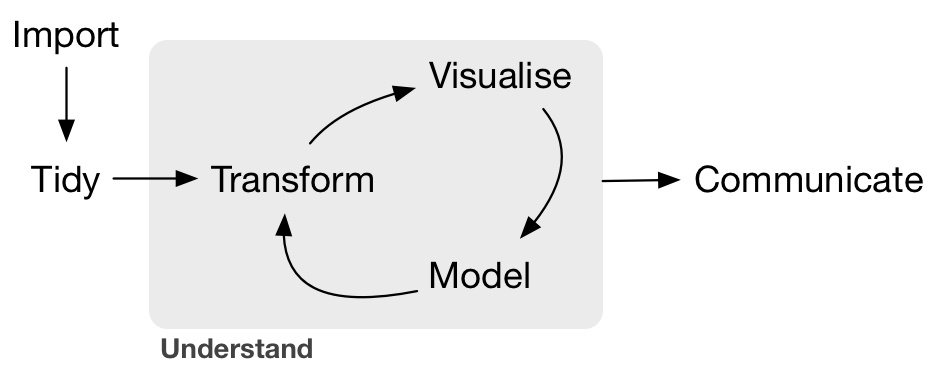
\includegraphics[width=\textwidth]{images/tidy1} 

}

\caption[Hadley's workflow graphic]{Hadley's workflow graphic}\label{fig:unnamed-chunk-3}
\end{figure}

We will begin with a discussion on what is meant by tidy data and then
dig into the gray \textbf{Understand} portion of the cycle and conclude
by talking about interpreting and discussing the results of our models
via \textbf{Communication}. These steps are vital to any statistical
analysis. But why should you care about statistics? ``Why did they make
me take this class?''

There's a reason so many fields require a statistics course. Scientific
knowledge grows through an understanding of statistical significance and
data analysis. You needn't be intimidated by statistics. It's not the
beast that it used to be and, paired with computation, you'll see how
reproducible research in the sciences particularly increases scientific
knowledge.

\section{Reproducibility}\label{reproducibility}

\begin{quote}
``The most important tool is the \emph{mindset}, when starting, that the
end product will be reproducible.'' -- Keith Baggerly
\end{quote}

Another large goal of this book is to help readers understand the
importance of reproducible analyses. The hope is to get readers into the
habit of making their analyses reproducible from the very beginning.
This means we'll be trying to help you build new habits. This will take
practice and be difficult at times. You'll see just why it is so
important for you to keep track of your code and well-document it to
help yourself later and any potential collaborators as well.

Copying and pasting results from one program into a word processor is
not the way that efficient and effective scientific research is
conducted. It's much more important for time to be spent on data
collection and data analysis and not on copying and pasting plots back
and forth across a variety of programs.

In a traditional analyses if an error was made with the original data,
we'd need to step through the entire process again: recreate the plots
and copy and paste all of the new plots and our statistical analysis
into your document. This is error prone and a frustrating use of time.
We'll see how to use R Markdown to get away from this tedious activity
so that we can spend more time doing science.

\begin{quote}
``We are talking about \emph{computational} reproducibility.'' - Yihui
Xie
\end{quote}

Reproducibility means a lot of things in terms of different scientific
fields. Are experiments conducted in a way that another researcher could
follow the steps and get similar results? In this book, we will focus on
what is known as \textbf{computational reproducibility}. This refers to
being able to pass all of one's data analysis, data sets, and
conclusions to someone else and have them get exactly the same results
on their machine. This allows for time to be spent doing actual science
and interpreting of results and assumptions instead of the more error
prone way of starting from scratch or following a list of steps that may
be different from machine to machine.

\section{Who is this book for?}\label{who-is-this-book-for}

This book is targeted at students taking a traditional intro stats class
in a small college environment using RStudio and preferably RStudio
Server. We assume no prerequisites: no algebra, no calculus, and no
prior programming experience. This is intended to be a gentle and nice
introduction to the practice of statistics in terms of how data
scientists, statisticians, data journalists, and other scientists
analyze data and write stories about data. We have intentionally avoided
the use of throwing formulas at you as much as possible and instead have
focused on developing statistical concepts via data visualization and
statistical computing. We hope this is a more intuitive experience than
the way statistics has traditionally been taught in the past (and how it
is commonly perceived from the outside). We additionally hope that you
see the value of reproducible research via R as you continue in your
studies. We understand that there will initially be growing pains in
learning to program but we are here to help you and you should know that
there is a huge community of R users that are always happy to help
newbies along as well.

Now let's get into learning about how to create good stories about and
with data!

\part{Data Exploration}\label{part-data-exploration}

\chapter{Tidy Data}\label{tidy}

In this chapter, we'll discuss the importance of tidy data. You may
think that this means just having your data in a spreadsheet, but you'll
see that it is actually more specific than that. Data actually comes to
us in a variety of formats from pictures to text to just numbers. We'll
focus on datasets that can be stored in a spreadsheet throughout this
book as that is the most common way data is collected in the sciences.

Having tidy data will allow us to more easily create data visualizations
as we will see in Chapter \ref{viz}. It will also help us with
manipulating data in Chapter \ref{manip} and in all subsequent chapters
when we discuss statistical inference. You may not necessarily
understand the importance for \textbf{tidy data} immediately but it will
become more and more apparent as we proceed through the book.

\subsection*{Needed packages}\label{needed-packages}
\addcontentsline{toc}{subsection}{Needed packages}

At the beginning of this and all subsequent chapters, we'll always have
a list of packages you should have installed and loaded. In particular
we load the \texttt{nycflights13} package which we'll discuss shortly
and the \texttt{dplyr} package for data manipulation, the subject of
Chapter \ref{manip}. We also load the \texttt{tibble} package here,
which contains the useful \texttt{glimpse} function.

\begin{Shaded}
\begin{Highlighting}[]
\KeywordTok{library}\NormalTok{(nycflights13)}
\KeywordTok{library}\NormalTok{(dplyr)}
\KeywordTok{library}\NormalTok{(tibble)}
\end{Highlighting}
\end{Shaded}

\section{What is tidy data?}\label{what-is-tidy-data}

You have surely heard the word ``tidy'' in your life:

\begin{itemize}
\tightlist
\item
  ``Tidy up your room!''
\item
  ``Please write your homework in a tidy way so that it is easier to
  grade and to provide feedback.''
\item
  Marie Kondo's best-selling book
  \href{https://www.amazon.com/Life-Changing-Magic-Tidying-Decluttering-Organizing/dp/1607747308/ref=sr_1_1?ie=UTF8\&qid=1469400636\&sr=8-1\&keywords=tidying+up}{\emph{The
  Life-Changing Magic of Tidying Up: The Japanese Art of Decluttering
  and Organizing}}
\item
  ``I am not by any stretch of the imagination a tidy person, and the
  piles of unread books on the coffee table and by my bed have a
  plaintive, pleading quality to me - `Read me, please!'\,'' - Linda
  Grant
\end{itemize}

So what does it mean for your data to be \textbf{tidy}? Put simply, it
means that your data is organized. But it's more than just that. It
means that your data follows the same standard format making it easy for
others to find elements of your data, to manipulate and transform your
data, and, for our purposes, continuing with the common theme: it makes
it easier to visualize your data and the relationships between different
variables in your data.

We will follow Hadley Wickham's definition of \textbf{tidy data} here
\citep{tidy}:

\begin{quote}
A dataset is a collection of values, usually either numbers (if
quantitative) or strings (if qualitative). Values are organised in two
ways. Every value belongs to a variable and an observation. A variable
contains all values that measure the same underlying attribute (like
height, temperature, duration) across units. An observation contains all
values measured on the same unit (like a person, or a day, or a race)
across attributes.
\end{quote}

\begin{quote}
Tidy data is a standard way of mapping the meaning of a dataset to its
structure. A dataset is messy or tidy depending on how rows, columns and
tables are matched up with observations, variables and types. In
\textbf{tidy data}:
\end{quote}

\begin{quote}
\begin{enumerate}
\def\labelenumi{\arabic{enumi}.}
\tightlist
\item
  Each variable forms a column.
\item
  Each observation forms a row.
\item
  Each type of observational unit forms a table.
\end{enumerate}
\end{quote}

\begin{figure}

{\centering 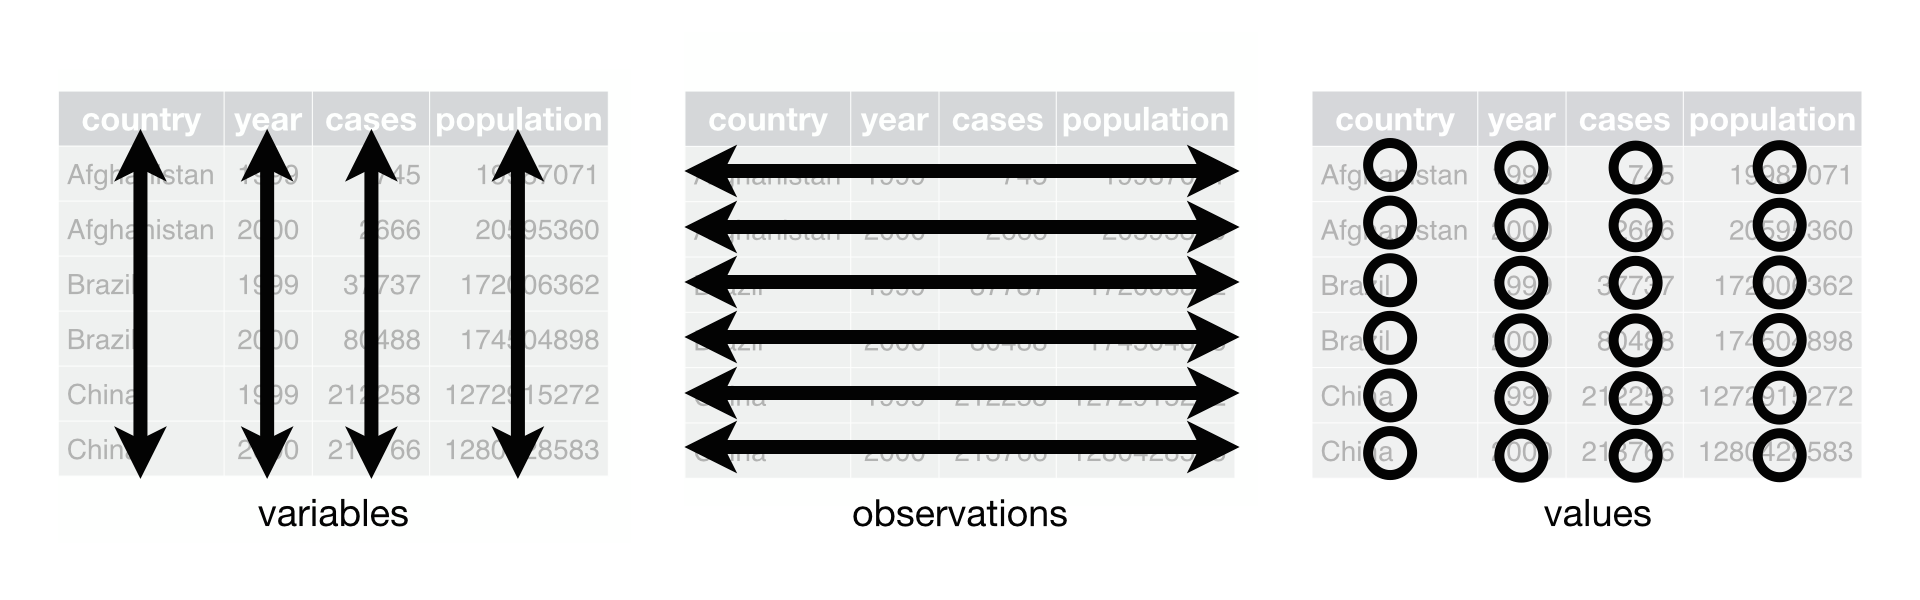
\includegraphics[width=\textwidth]{images/tidy-1} 

}

\caption[Tidy data graphic from http://r4ds.had.co.nz/tidy-data.html]{Tidy data graphic from http://r4ds.had.co.nz/tidy-data.html}\label{fig:tidyfig}
\end{figure}

Reading over this definition, you can begin to think about datasets that
won't follow this nice format. This format of data is also known as
``long'' format.

\begin{center}\rule{0.5\linewidth}{\linethickness}\end{center}

\begin{learncheck}
\textbf{\emph{Learning check}}
\end{learncheck}

\textbf{(LC3.1)} Give an example dataset that doesn't follow this
format.

\begin{itemize}
\tightlist
\item
  What features of this dataset might make it difficult to visualize?\\
\item
  How could the dataset be tweaked to make it \textbf{tidy}?
\end{itemize}

\textbf{(LC3.2)} Say the following table are stock prices, how would you
make this tidy?

\begin{tabular}{l|l|l|l}
\hline
Date & Boeing & Amazon & Google\\
\hline
2009-01-01 & \$173.55 & \$174.90 & \$174.34\\
\hline
2009-01-02 & \$172.61 & \$171.42 & \$170.04\\
\hline
2009-01-03 & \$173.86 & \$171.58 & \$173.65\\
\hline
2009-01-04 & \$170.77 & \$173.89 & \$174.87\\
\hline
2009-01-05 & \$174.29 & \$170.16 & \$172.19\\
\hline
\end{tabular}

\begin{center}\rule{0.5\linewidth}{\linethickness}\end{center}

\section{\texorpdfstring{Datasets in the \texttt{nycflights13}
package}{Datasets in the nycflights13 package}}\label{datasets-in-the-nycflights13-package}

We likely have all flown on airplanes or know someone that has. Air
travel has become an ever-present aspect of our daily lives. If you live
in or are visiting a relatively large city and you walk around that
city's airport, you see gates showing flight information from many
different airlines. And you will frequently see that some flights are
delayed because of a variety of conditions. Are there ways that we can
avoid having to deal with these flight delays?

We'd all like to arrive at our destinations on time whenever possible.
(Unless you secretly love hanging out at airports. If you are one of
these people, pretend for the moment that you are very much anticipating
being at your final destination.) Throughout this book, we're going to
analyze data related to flights contained in the \texttt{nycflights13}
package we loaded earlier \citep{R-nycflights13}. Specifically, this
package contains information about all flights that departed from NYC
(e.g.~EWR, JFK and LGA) in 2013 in 5 data sets:

\begin{itemize}
\tightlist
\item
  \texttt{flights}: information on all 336,776 flights
\item
  \texttt{weather}: hourly meterological data for each airport
\item
  \texttt{planes}: construction information about each plane
\item
  \texttt{airports}: airport names and locations
\item
  \texttt{airlines}: translation between two letter carrier codes and
  names
\end{itemize}

We will begin by loading in the \texttt{flights} dataset and getting an
idea of its structure. Run the following in your console

\begin{Shaded}
\begin{Highlighting}[]
\KeywordTok{data}\NormalTok{(flights)}
\end{Highlighting}
\end{Shaded}

This line of code loads in the \texttt{flights} dataset that is stored
in the \texttt{nycflights13} package. This dataset and most others
presented in this book will be in the ``data frame'' format in R. Data
frames are essentially spreadsheets and allow us to look at collections
of variables that are tightly coupled together.

The best way to get a feel for a data frame is to use the \texttt{View}
function in RStudio. This command will be given throughout the book as a
reminder, but the actual output will be hidden. Run
\texttt{View(flights)} in R and look over this data frame. You should
slowly get into the habit of always \texttt{View}ing any data frames
that come your way.

\begin{center}\rule{0.5\linewidth}{\linethickness}\end{center}

\begin{learncheck}
\textbf{\emph{Learning check}}
\end{learncheck}

\textbf{(LC3.3)} What does any \emph{ONE} row in this \texttt{flights}
dataset refer to?

\begin{itemize}
\tightlist
\item
  A. Data on an airline
\item
  B. Data on a flight
\item
  C. Data on an airport
\item
  D. Data on multiple flights
\end{itemize}

\begin{center}\rule{0.5\linewidth}{\linethickness}\end{center}

By running \texttt{View(flights)}, we see the different
\textbf{variables} listed in the columns and we see that there are
different types of variables. Some of the variables like
\texttt{distance}, \texttt{day}, and \texttt{arr\_delay} are what we
will call \textbf{quantitative} variables. These variables vary in a
numerical way. Other variables here are \textbf{categorical}.

Note that if you look in the leftmost column of the
\texttt{View(flights)} output, you will see a column of numbers. These
are the row numbers of the dataset. If you glance across a row with the
same number, say row 5, you can get an idea of what each row corresponds
to. In other words, this will allow you to identify what object is being
referred to in a given row. This is often called the
\textbf{observational unit}. The \textbf{observational unit} in this
example is an individual flight departing New York City in 2013. You can
identify the observational unit by determining what the \textbf{thing}
is that is being measured in each of the variables.

\textbf{Note}: Frequently the first thing you should do when given a
dataset is to

\begin{itemize}
\tightlist
\item
  identify the observational unit,
\item
  specify the variables, and
\item
  give the types of variables you are presented with.
\end{itemize}

The \texttt{glimpse()} command in the \texttt{tibble} package provides
us with much of the above information and more:

\begin{Shaded}
\begin{Highlighting}[]
\KeywordTok{glimpse}\NormalTok{(flights)}
\end{Highlighting}
\end{Shaded}

\begin{verbatim}
## Observations: 336,776
## Variables: 19
## $ year           <int> 2013, 2013, 2013, 2013, 2013, 2013, 2013, 20...
## $ month          <int> 1, 1, 1, 1, 1, 1, 1, 1, 1, 1, 1, 1, 1, 1, 1,...
## $ day            <int> 1, 1, 1, 1, 1, 1, 1, 1, 1, 1, 1, 1, 1, 1, 1,...
## $ dep_time       <int> 517, 533, 542, 544, 554, 554, 555, 557, 557,...
## $ sched_dep_time <int> 515, 529, 540, 545, 600, 558, 600, 600, 600,...
## $ dep_delay      <dbl> 2, 4, 2, -1, -6, -4, -5, -3, -3, -2, -2, -2,...
## $ arr_time       <int> 830, 850, 923, 1004, 812, 740, 913, 709, 838...
## $ sched_arr_time <int> 819, 830, 850, 1022, 837, 728, 854, 723, 846...
## $ arr_delay      <dbl> 11, 20, 33, -18, -25, 12, 19, -14, -8, 8, -2...
## $ carrier        <chr> "UA", "UA", "AA", "B6", "DL", "UA", "B6", "E...
## $ flight         <int> 1545, 1714, 1141, 725, 461, 1696, 507, 5708,...
## $ tailnum        <chr> "N14228", "N24211", "N619AA", "N804JB", "N66...
## $ origin         <chr> "EWR", "LGA", "JFK", "JFK", "LGA", "EWR", "E...
## $ dest           <chr> "IAH", "IAH", "MIA", "BQN", "ATL", "ORD", "F...
## $ air_time       <dbl> 227, 227, 160, 183, 116, 150, 158, 53, 140, ...
## $ distance       <dbl> 1400, 1416, 1089, 1576, 762, 719, 1065, 229,...
## $ hour           <dbl> 5, 5, 5, 5, 6, 5, 6, 6, 6, 6, 6, 6, 6, 6, 6,...
## $ minute         <dbl> 15, 29, 40, 45, 0, 58, 0, 0, 0, 0, 0, 0, 0, ...
## $ time_hour      <dttm> 2013-01-01 05:00:00, 2013-01-01 05:00:00, 2...
\end{verbatim}

\begin{center}\rule{0.5\linewidth}{\linethickness}\end{center}

\begin{learncheck}
\textbf{\emph{Learning check}}
\end{learncheck}

\textbf{(LC3.4)} What are some examples in this dataset of
\textbf{categorical} variables? What makes them different than
\textbf{quantitative} variables?

\textbf{(LC3.5)} What does \texttt{int}, \texttt{dbl}, and \texttt{chr}
mean in the output above? If you need a hint, you might want to run
\texttt{str(flights)} instead.

\textbf{(LC3.6)} How many different columns are in this dataset?

\textbf{(LC3.7)} How many different rows are in this dataset?

\begin{center}\rule{0.5\linewidth}{\linethickness}\end{center}

We see that \texttt{glimpse} will give you the first few entries of each
variable in a row after the variable. In addition, the type of the
variable is given immediately after each variable's name inside
\texttt{\textless{}\ \textgreater{}}. Here, \texttt{int} and
\texttt{num} refer to quantitative variables. In contrast, \texttt{chr}
refers to categorical variables. One more type of variable is given here
with the \texttt{time\_hour} variable: \textbf{dttm}. As you may
suspect, this variable corresponds to a specific date and time of day.

Another nice feature of R is the help system. You can get help in R by
simply entering a question mark before the name of a function or an
object and you will be presented with a page showing the documentation.
Since \texttt{glimpse} is a function defined in the \texttt{tibble}
package, you can further emphasize that you'd like to look at the help
for that specific \texttt{glimpse} function by adding the two columns
between the package name and the function. Note that these output help
files is omitted here but the \texttt{flights} help can be accessed
\href{https://cran.r-project.org/web/packages/nycflights13/nycflights13.pdf}{here}
on page 3 of the PDF document.

\begin{Shaded}
\begin{Highlighting}[]
\NormalTok{?tibble::glimpse}
\NormalTok{?flights}
\end{Highlighting}
\end{Shaded}

Another aspect of tidy data is a description of what each variable in
the dataset represents. This helps others to understand what your
variable names mean and what they correspond to. If we look at the
output of \texttt{?flights}, we can see that a description of each
variable by name is given.

An important feature to \textbf{ALWAYS} include with your data is the
appropriate units of measurement. We'll see this further when we work
with the \texttt{dep\_delay} variable in Chapter \ref{viz}. (It's in
minutes, but you'd get some really strange interpretations if you
thought it was in hours or seconds. UNITS MATTER!)

\section{\texorpdfstring{How is \texttt{flights}
tidy?}{How is flights tidy?}}\label{how-is-flights-tidy}

We see that \texttt{flights} has a rectangular shape with each row
corresponding to a different flight and each column corresponding to a
characteristic of that flight. This matches exactly with how Hadley
Wickham defined tidy data:

\begin{enumerate}
\def\labelenumi{\arabic{enumi}.}
\tightlist
\item
  Each variable forms a column.
\item
  Each observation forms a row.
\end{enumerate}

But what about the third property?

\begin{quote}
\begin{enumerate}
\def\labelenumi{\arabic{enumi}.}
\setcounter{enumi}{2}
\tightlist
\item
  Each type of observational unit forms a table.
\end{enumerate}
\end{quote}

We identified earlier that the observational unit in the
\texttt{flights} dataset is an individual flight. And we have shown that
this dataset consists of 336,776 flights with 19 variables. In other
words, some rows of this dataset don't refer to a measurement on an
airline or on an airport. They specifically refer to
characteristics/measurements on a given \textbf{flight} from New York
City in 2013.

By contrast, also included in the \texttt{nycflights13} package are
datasets with different observational units \citep{R-nycflights13}:

\begin{itemize}
\tightlist
\item
  \texttt{weather}: hourly meteorological data for each airport
\item
  \texttt{planes}: construction information about each plane
\item
  \texttt{airports}: airport names and locations
\item
  \texttt{airlines}: translation between two letter carrier codes and
  names
\end{itemize}

You may have been asking yourself what \texttt{carrier} refers to in the
\texttt{glimpse(flights)} output above. The \texttt{airlines} dataset
provides a description of this with each airline being the observational
unit:

\begin{Shaded}
\begin{Highlighting}[]
\KeywordTok{data}\NormalTok{(airlines)}
\NormalTok{airlines}
\end{Highlighting}
\end{Shaded}

\begin{verbatim}
## # A tibble: 16 × 2
##    carrier                        name
##      <chr>                       <chr>
## 1       9E           Endeavor Air Inc.
## 2       AA      American Airlines Inc.
## 3       AS        Alaska Airlines Inc.
## 4       B6             JetBlue Airways
## 5       DL        Delta Air Lines Inc.
## 6       EV    ExpressJet Airlines Inc.
## 7       F9      Frontier Airlines Inc.
## 8       FL AirTran Airways Corporation
## 9       HA      Hawaiian Airlines Inc.
## 10      MQ                   Envoy Air
## 11      OO       SkyWest Airlines Inc.
## 12      UA       United Air Lines Inc.
## 13      US             US Airways Inc.
## 14      VX              Virgin America
## 15      WN      Southwest Airlines Co.
## 16      YV          Mesa Airlines Inc.
\end{verbatim}

As can be seen here when you just enter the name of an object in R, by
default it will print the contents of that object to the screen. Be
careful! It's usually better to use the \texttt{View()} function in
RStudio since larger objects may take awhile to print to the screen and
it likely won't be helpful to you to have hundreds of lines outputted.

\begin{center}\rule{0.5\linewidth}{\linethickness}\end{center}

\begin{learncheck}
\textbf{\emph{Learning check}}
\end{learncheck}

\textbf{(LC3.8)} Run the following block of code in RStudio to load and
view each of the four data frames in the \texttt{nycflights13} package.
Switch between the different tabs that have opened to view each of the
four data frames. Describe in two sentences for each data frame what
stands out to you and what the most important features are of each.

\begin{Shaded}
\begin{Highlighting}[]
\KeywordTok{data}\NormalTok{(weather)}
\KeywordTok{data}\NormalTok{(planes)}
\KeywordTok{data}\NormalTok{(airports)}
\KeywordTok{data}\NormalTok{(airlines)}
\KeywordTok{View}\NormalTok{(weather)}
\KeywordTok{View}\NormalTok{(planes)}
\KeywordTok{View}\NormalTok{(airports)}
\KeywordTok{View}\NormalTok{(airlines)}
\end{Highlighting}
\end{Shaded}

\begin{center}\rule{0.5\linewidth}{\linethickness}\end{center}

\subsection{Identification variables}\label{identification-variables}

There is a subtle difference between the kinds of variables that you
will encounter in data frames. The \texttt{airports} data frame you
worked with above contains data in these different kinds. Let's pull
them apart using the \texttt{glimpse} function:

\begin{Shaded}
\begin{Highlighting}[]
\KeywordTok{glimpse}\NormalTok{(airports)}
\end{Highlighting}
\end{Shaded}

\begin{verbatim}
## Observations: 1,458
## Variables: 8
## $ faa   <chr> "04G", "06A", "06C", "06N", "09J", "0A9", "0G6", "0G7...
## $ name  <chr> "Lansdowne Airport", "Moton Field Municipal Airport",...
## $ lat   <dbl> 41.13, 32.46, 41.99, 41.43, 31.07, 36.37, 41.47, 42.8...
## $ lon   <dbl> -80.62, -85.68, -88.10, -74.39, -81.43, -82.17, -84.5...
## $ alt   <int> 1044, 264, 801, 523, 11, 1593, 730, 492, 1000, 108, 4...
## $ tz    <dbl> -5, -6, -6, -5, -5, -5, -5, -5, -5, -8, -5, -6, -5, -...
## $ dst   <chr> "A", "A", "A", "A", "A", "A", "A", "A", "U", "A", "A"...
## $ tzone <chr> "America/New_York", "America/Chicago", "America/Chica...
\end{verbatim}

The variables \texttt{faa} and \texttt{name} are what we will call
\emph{identification variables}. They are mainly used to provide a name
to the observational unit. Here the observational unit is an airport and
the \texttt{faa} gives the code provided by the FAA for that airport
while the \texttt{name} variable gives the longer more natural name of
the airport. These ID variables differ from the other variables that are
often called \emph{measurement} or \emph{characteristic} variables. The
remaining variables (aside from \texttt{faa} and \texttt{name}) are of
this type in \texttt{airports}. They don't uniquely identify the
observational unit, but instead describe properties of the observational
unit. For organizational purposes, it is best practice to have your
identification variables in the far leftmost columns of your data frame.

\begin{center}\rule{0.5\linewidth}{\linethickness}\end{center}

\begin{learncheck}
\textbf{\emph{Learning check}}
\end{learncheck}

\textbf{(LC3.9)} What properties of the observational unit do each of
\texttt{lat}, \texttt{lon}, \texttt{alt}, \texttt{tz}, \texttt{dst}, and
\texttt{tzone} describe for the \texttt{airports} data frame? Note that
you may want to use \texttt{?airports} to get more information or go to
the reference manual for the \texttt{nycflights13} package
\href{https://cran.r-project.org/web/packages/nycflights13/nycflights13.pdf}{here}.

\textbf{(LC3.10)} Provide the names of variables in a data frame with at
least three variables in which one of them is an identification variable
and the other two are not. In other words, create your own tidy data set
that matches these conditions.

\begin{center}\rule{0.5\linewidth}{\linethickness}\end{center}

\section{Normal forms of data}\label{normal-forms-of-data}

The datasets included in the \texttt{nycflights13} package are in a form
that minimizes redundancy of data. We will see that there are ways to
\emph{merge} (or \emph{join}) the different tables together easily. We
are capable of doing so because each of the tables have \emph{keys} in
common to relate one to another. This is an important property of
\textbf{normal forms} of data. The process of decomposing data frames
into less redundant tables without losing information is called
\textbf{normalization}. More information is available on
\href{https://en.wikipedia.org/wiki/Database_normalization}{Wikipedia}.

We saw an example of this above with the \texttt{airlines} dataset.
While the \texttt{flights} data frame could also include a column with
the names of the airlines instead of the carrier code, this would be
repetitive since there is a unique mapping of the carrier code to the
name of the airline/carrier.

Below an example is given showing how to \textbf{join} the
\texttt{airlines} data frame together with the \texttt{flights} data
frame by linking together the two datasets via a common \textbf{key} of
\texttt{"carrier"}. Note that this ``joined'' data frame is assigned to
a new data frame called \texttt{joined\_flights}. The \textbf{key}
variable that we frequently join by is one of the \emph{identification
variables} mentioned above.

\begin{Shaded}
\begin{Highlighting}[]
\KeywordTok{library}\NormalTok{(dplyr)}
\NormalTok{joined_flights <-}\StringTok{ }\KeywordTok{inner_join}\NormalTok{(}\DataTypeTok{x =} \NormalTok{flights, }\DataTypeTok{y =} \NormalTok{airlines, }\DataTypeTok{by =} \StringTok{"carrier"}\NormalTok{)}
\end{Highlighting}
\end{Shaded}

\begin{Shaded}
\begin{Highlighting}[]
\KeywordTok{View}\NormalTok{(joined_flights)}
\end{Highlighting}
\end{Shaded}

If we \texttt{View} this dataset, we see a new variable has been created
called \texttt{name}. (We will see in Subsection \ref{rename} ways to
change \texttt{name} to a more descriptive variable name.) More
discussion about joining data frames together will be given in Chapter
\ref{manip}. We will see there that the names of the columns to be
linked need not match as they did here with \texttt{"carrier"}.

\begin{center}\rule{0.5\linewidth}{\linethickness}\end{center}

\begin{learncheck}
\textbf{\emph{Learning check}}
\end{learncheck}

\textbf{(LC3.11)} What are common characteristics of ``tidy'' datasets?

\textbf{(LC3.12)} What makes ``tidy'' datasets useful for organizing
data?

\textbf{(LC3.13)} How many variables are presented in the table below?
What does each row correspond to? (\textbf{Hint:} You may not be able to
answer both of these questions immediately but take your best guess.)

\begin{tabular}{r|r}
\hline
students & faculty\\
\hline
4 & 2\\
\hline
6 & 3\\
\hline
\end{tabular}

\textbf{(LC3.14)} The confusion you may have encountered in LC3.13 is a
common one those that work with data are commonly presented with. This
dataset is not tidy. Actually, the dataset in LC3.13 has three variables
not the two that were presented. Make a guess as to what these variables
are and present a tidy dataset instead of this untidy one given in
LC3.13.

\textbf{(LC3.15)} The actual data presented in LC3.13 is given below in
tidy data format:

\begin{tabular}{l|l|l}
\hline
role & Sociology? & Type of School\\
\hline
student & TRUE & Public\\
\hline
student & TRUE & Public\\
\hline
student & TRUE & Public\\
\hline
student & TRUE & Public\\
\hline
student & FALSE & Public\\
\hline
student & FALSE & Public\\
\hline
student & FALSE & Private\\
\hline
student & FALSE & Private\\
\hline
student & FALSE & Private\\
\hline
student & FALSE & Private\\
\hline
faculty & TRUE & Public\\
\hline
faculty & TRUE & Public\\
\hline
faculty & FALSE & Public\\
\hline
faculty & FALSE & Private\\
\hline
faculty & FALSE & Private\\
\hline
\end{tabular}

\begin{itemize}
\tightlist
\item
  What does each row correspond to?\\
\item
  What are the different variables in this data frame?\\
\item
  The \texttt{Sociology?} variable is known as a logical variable. What
  types of values does a logical variable take on?
\end{itemize}

\textbf{(LC3.16)} What are some advantages of data in normal forms? What
are some disadvantages?

\begin{center}\rule{0.5\linewidth}{\linethickness}\end{center}

\begin{center}\rule{0.5\linewidth}{\linethickness}\end{center}

\begin{review}
\textbf{\emph{Review questions}}
\end{review}

Review questions have been designed using the \texttt{fivethirtyeight} R
package \citep{R-fivethirtyeight} with links to the corresponding
FiveThirtyEight.com articles in our free DataCamp course
\textbf{Effective Data Storytelling using the \texttt{tidyverse}}. The
material in this chapter is covered in the \textbf{Tidy Data} chapter of
the DataCamp course available
\href{https://campus.datacamp.com/courses/effective-data-storytelling-using-the-tidyverse/tidy-data}{here}.

\begin{center}\rule{0.5\linewidth}{\linethickness}\end{center}

\begin{center}\rule{0.5\linewidth}{\linethickness}\end{center}

\section{What's to come?}\label{whats-to-come}

In Chapter \ref{viz}, we will further explore the distribution of a
variable in a related dataset to \texttt{flights}: the \texttt{temp}
variable in the \texttt{weather} dataset. We'll be interested in
understanding how this variable varies in relation to the values of
other variables in the dataset. We will see that visualization is often
a powerful tool in helping us see what is going on in a dataset. It will
be a useful way to expand on the \texttt{glimpse} function we have seen
here for tidy data.

\chapter{Data Visualization via ggplot2}\label{viz}

In Chapter \ref{tidy}, we discussed the importance of datasets being
\textbf{tidy}. You will see in examples here why having a tidy dataset
helps us immensely when plotting our data. In plotting our data, we will
be able to gain valuable insights from our data that we couldn't
initially see from just looking at the raw data. We will focus on using
Hadley Wickham's \texttt{ggplot2} package in doing so, which was
developed to work specifically on datasets that are \textbf{tidy}. It
provides an easy way to customize your plots and is based on data
visualization theory given in \emph{The Grammar of Graphics}
\citep{wilkinson2005}.

At the most basic level, graphics/plots/charts provide a nice way for us
to get a sense for how quantitative variables compare in terms of their
center and their spread. The most important thing to know about graphics
is that they should be created to make it obvious for your audience to
see the findings you want to get across. This requires a balance of not
including too much in your plots, but also including enough so that
relationships and interesting findings can be easily seen. As we will
see, plots/graphics also help us to identify patterns and outliers in
our data. We will see that a common extension of these ideas is to
compare the \textbf{distribution} of one quantitative variable (i.e.,
what the spread of a variable looks like or how the variable is
\emph{distributed} in terms of its values) as we go across the levels of
a different categorical variable.

\subsection*{Needed packages}\label{needed-packages-1}
\addcontentsline{toc}{subsection}{Needed packages}

Before we proceed with this chapter, let's load all the necessary
packages.

\begin{Shaded}
\begin{Highlighting}[]
\KeywordTok{library}\NormalTok{(ggplot2)}
\KeywordTok{library}\NormalTok{(nycflights13)}
\KeywordTok{library}\NormalTok{(knitr)}
\KeywordTok{library}\NormalTok{(dplyr)}
\end{Highlighting}
\end{Shaded}

\section{The Grammar of Graphics}\label{grammarofgraphics}

We begin with a discussion of a theoretical framework for data
visualization known as the ``The Grammar of Graphics,'' which serves as
the basis for the \texttt{ggplot2} package. Much like the way we
construct sentences in any language using a linguistic grammar (nouns,
verbs, subjects, objects, etc.), the theoretical framework given by
Leland Wilkinson \citep{wilkinson2005} allows us to specify the
components of a statistical graphic.

\subsection{Components of Grammar}\label{components-of-grammar}

In short, the grammar tells us that:

\begin{quote}
\textbf{A statistical graphic is a mapping of \texttt{data} variables to
\texttt{aes}thetic attributes of \texttt{geom}etric objects.}
\end{quote}

Specifically, we can break a graphic into the following three essential
components:

\begin{enumerate}
\def\labelenumi{\arabic{enumi}.}
\tightlist
\item
  \texttt{data}: the data set comprised of variables that we map.
\item
  \texttt{geom}: the geometric object in question. This refers to our
  type of objects we can observe in our plot. For example, points,
  lines, bars, etc.
\item
  \texttt{aes}: aesthetic attributes of the geometric object that we can
  perceive on a graphic. For example, x/y position, color, shape, and
  size. Each assigned aesthetic attribute can be mapped to a variable in
  our data set. If not assigned, they are set to defaults.
\end{enumerate}

\subsection{Napolean's March on Moscow}\label{napoleans-march-on-moscow}

In 1812, Napoleon led a French invasion of Russia, marching on Moscow.
It was one of the biggest military disasters due in large part to the
Russian winter. In 1869, a French civil engineer named Charles Joseph
Minard published arguably one of the greatest statistical visualizations
of all-time, which summarized this march:

\begin{figure}

{\centering 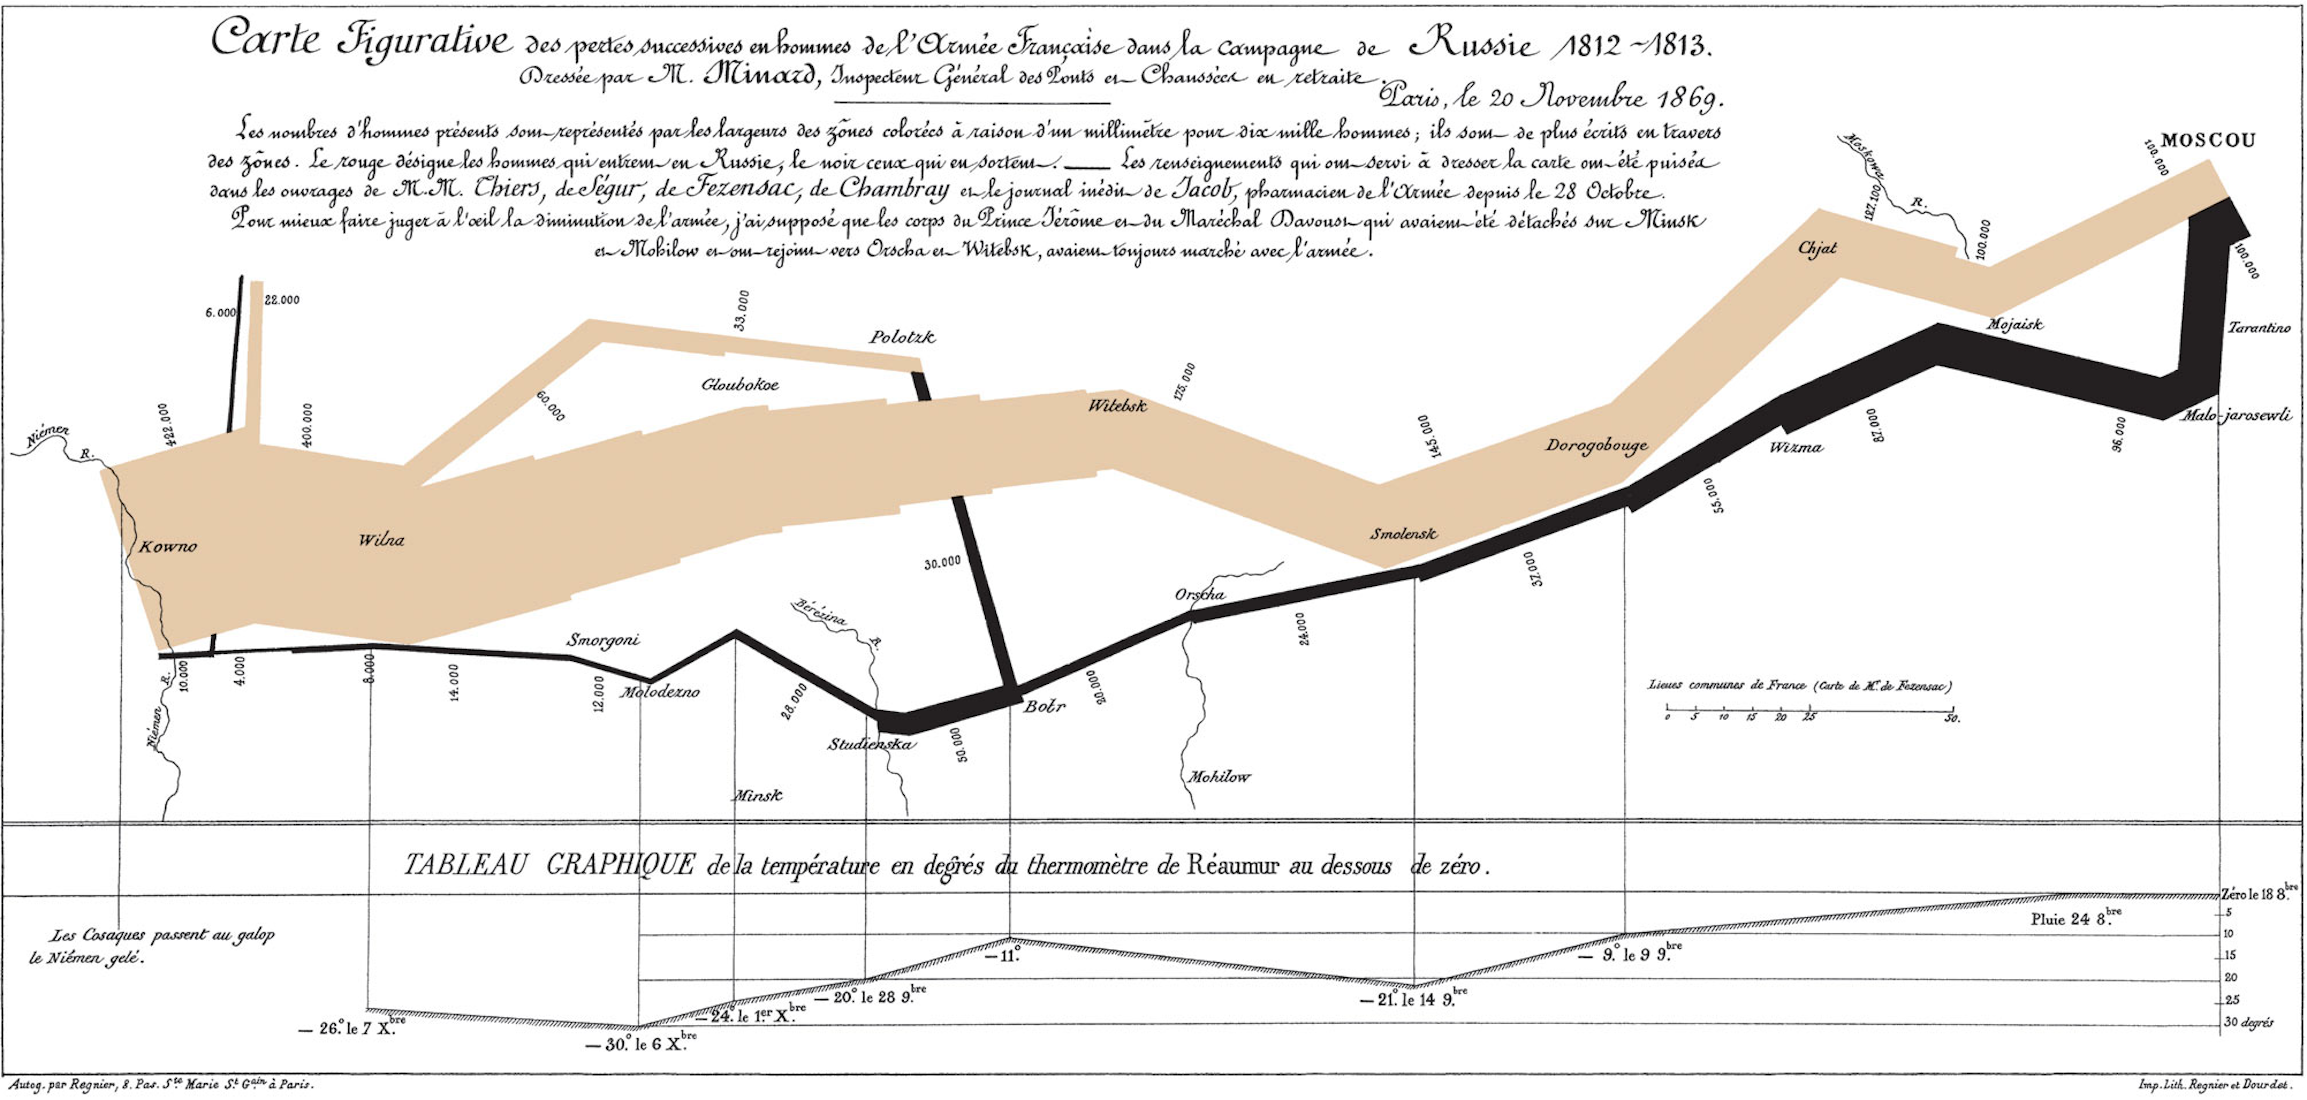
\includegraphics[width=\textwidth]{images/Minard} 

}

\caption[Minard's Visualization of Napolean's March]{Minard's Visualization of Napolean's March}\label{fig:minard}
\end{figure}

This was considered a revolution in statistical graphics because between
the map on top and the line graph on the bottom, there are 6 dimensions
of information (i.e.~variables) being displayed on a 2-dimensional page.
Let's view this graphic through the lens of the Grammar of Graphics:

\begin{table}
\caption{\label{tab:unnamed-chunk-17}Grammar of Map (Top) and Line-Graph (Bottom) in Minard's Graphic of Napolean's March}

\centering
\begin{tabular}[t]{lll}
\toprule
data & aes & geom\\
\midrule
longitude & x & point\\
latitude & y & point\\
army size & size & path\\
army direction & color & path\\
\bottomrule
\end{tabular}
\centering
\begin{tabular}[t]{lll}
\toprule
data & aes & geom\\
\midrule
date & x & line \& text\\
temperature & y & line \& text\\
\bottomrule
\end{tabular}
\end{table}

For example, the data variable \texttt{longitude} gets mapped to the
\texttt{x} \texttt{aes}thetic of the points \texttt{geom}etric objects
on the map while the annotated line-graph displays \texttt{date} and
\texttt{temperature} variable information via its mapping to the
\texttt{x} and \texttt{y} \texttt{aes}thetic of the line
\texttt{geom}etric object.

\subsection{Other Components of the
Grammar}\label{other-components-of-the-grammar}

There are other components of the Grammar of Graphics we can control:

\begin{itemize}
\tightlist
\item
  \texttt{facet}: how to break up a plot into subsets
\item
  \texttt{stat}istical transformations: this includes smoothing, binning
  values into a histogram, or just itself un-transformed as
  \texttt{"identity"}.
\item
  \texttt{scales} both

  \begin{itemize}
  \tightlist
  \item
    convert \textbf{data units} to \textbf{physical units} the computer
    can display
  \item
    draw a legend and/or axes, which provide an inverse mapping to make
    it possible to read the original data values from the graph.
  \end{itemize}
\item
  \texttt{coord}inate system for x/y values: typically
  \texttt{cartesian}, but can also be \texttt{polar} or \texttt{map}
\item
  \texttt{position} adjustments
\end{itemize}

In this text, we will only focus on the first two: \texttt{facet}ing
(introduced in Section \ref{facets}) and \texttt{stat}istical
transformations (in a limited sense, when consider Barplots in Section
\ref{geombar}); the other components are left to a more advanced text.
This is not a problem when producing a plot as each of these components
have default settings.

There are other extra attributes that can be tweaked as well including
the plot title, axes labels, and over-arching themes for the plot. In
general, the Grammar of Graphics allows for customization but also a
consistent framework that allows the user to easily tweak their
creations as needed in order to convey a message about their data.

\subsection{The ggplot2 Package}\label{the-ggplot2-package}

We next introduce Hadley Wickham's \texttt{ggplot2} package, which is an
implementation of the Grammar of Graphics for R \citep{R-ggplot2}. You
may have noticed that a lot of previous text in this chapter is written
in computer font. This is because the various components of the Grammar
of Graphics are specified using the \texttt{ggplot} function, which
expects at a bare minimal as arguments

\begin{itemize}
\tightlist
\item
  the data frame where the variables exist (the \texttt{data} argument)
  and
\item
  the names of the variables to be plotted (the \texttt{mapping}
  argument).
\end{itemize}

The names of the variables will be entered into the \texttt{aes}
function as arguments where \texttt{aes} stands for ``aesthetics''.

\section{Five Named Graphs - The 5NG}\label{five-named-graphs---the-5ng}

For our purposes, we will be limiting consideration to five different
types of graphs (note that in this text we use the terms ``graphs'',
``plots'', and ``charts'' interchangeably). We term these five named
graphs the \textbf{5NG}:

\begin{enumerate}
\def\labelenumi{\arabic{enumi}.}
\tightlist
\item
  scatter-plots
\item
  line-graphs
\item
  boxplots
\item
  histograms
\item
  barplots
\end{enumerate}

With this repertoire of plots, you can visualize a wide array of data
variables thrown at you. We will discuss some variations of these, but
with the 5NG in your toolbox you can do big things! Something we will
also stress here is that certain plots only work for categorical/logical
variables and others only for quantitative variables. You'll want to
quiz yourself often as we go along on which plot makes sense a given a
particular problem set-up.

\section{5NG\#1: Scatter-plots}\label{scatterplots}

The simplest of the 5NG are \textbf{scatter-plots} (also called
bivariate plots); they allow you to investigate the relationship between
two continuous variables. While you may already be familiar with such
plots, let's view it through the lens of the Grammar of Graphics.
Specifically, we will graphically investigate the relationship between
the following two continuous variables in the \texttt{flights} data
frame:

\begin{enumerate}
\def\labelenumi{\arabic{enumi}.}
\tightlist
\item
  \texttt{dep\_delay}: departure delay on the horizontal ``x'' axis and
\item
  \texttt{arr\_delay}: arrival delay on the vertical ``y'' axis
\end{enumerate}

for Alaska Airlines flights leaving NYC in 2013. This requires paring
down the \texttt{flights} data frame to a smaller data frame
\texttt{all\_alaska\_flights} consisting of only Alaska Airlines
(carrier code ``AS'') flights.

\begin{Shaded}
\begin{Highlighting}[]
\KeywordTok{data}\NormalTok{(flights)}
\NormalTok{all_alaska_flights <-}\StringTok{ }\NormalTok{flights %>%}\StringTok{ }
\StringTok{  }\KeywordTok{filter}\NormalTok{(carrier ==}\StringTok{ "AS"}\NormalTok{)}
\end{Highlighting}
\end{Shaded}

This code snippet makes use of functions in the \texttt{dplyr} package
for data manipulation to achieve our goal: it takes the \texttt{flights}
data frame and \texttt{filter}s it to only return the rows which meet
the condition \texttt{carrier\ ==\ "AS"} (recall equality is specified
with \texttt{==} and not \texttt{=}). You will see many more examples
using this function in Chapter \ref{manip}.

\begin{center}\rule{0.5\linewidth}{\linethickness}\end{center}

\begin{learncheck}
\textbf{\emph{Learning check}}
\end{learncheck}

\textbf{(LC4.1)} Take a look at both the \texttt{flights} and
\texttt{all\_alaska\_flights} data frames by running
\texttt{View(flights)} and \texttt{View(all\_alaska\_flights)} in the
console. In what respect do these data frames differ?

\begin{center}\rule{0.5\linewidth}{\linethickness}\end{center}

\subsection{Scatter-plots via geom\_point}\label{geompoint}

We proceed to create the scatter-plot using the \texttt{ggplot()}
function:

\begin{Shaded}
\begin{Highlighting}[]
\KeywordTok{ggplot}\NormalTok{(}\DataTypeTok{data =} \NormalTok{all_alaska_flights, }\KeywordTok{aes}\NormalTok{(}\DataTypeTok{x =} \NormalTok{dep_delay, }\DataTypeTok{y =} \NormalTok{arr_delay)) +}\StringTok{ }
\StringTok{  }\KeywordTok{geom_point}\NormalTok{()}
\end{Highlighting}
\end{Shaded}

\begin{figure}

{\centering 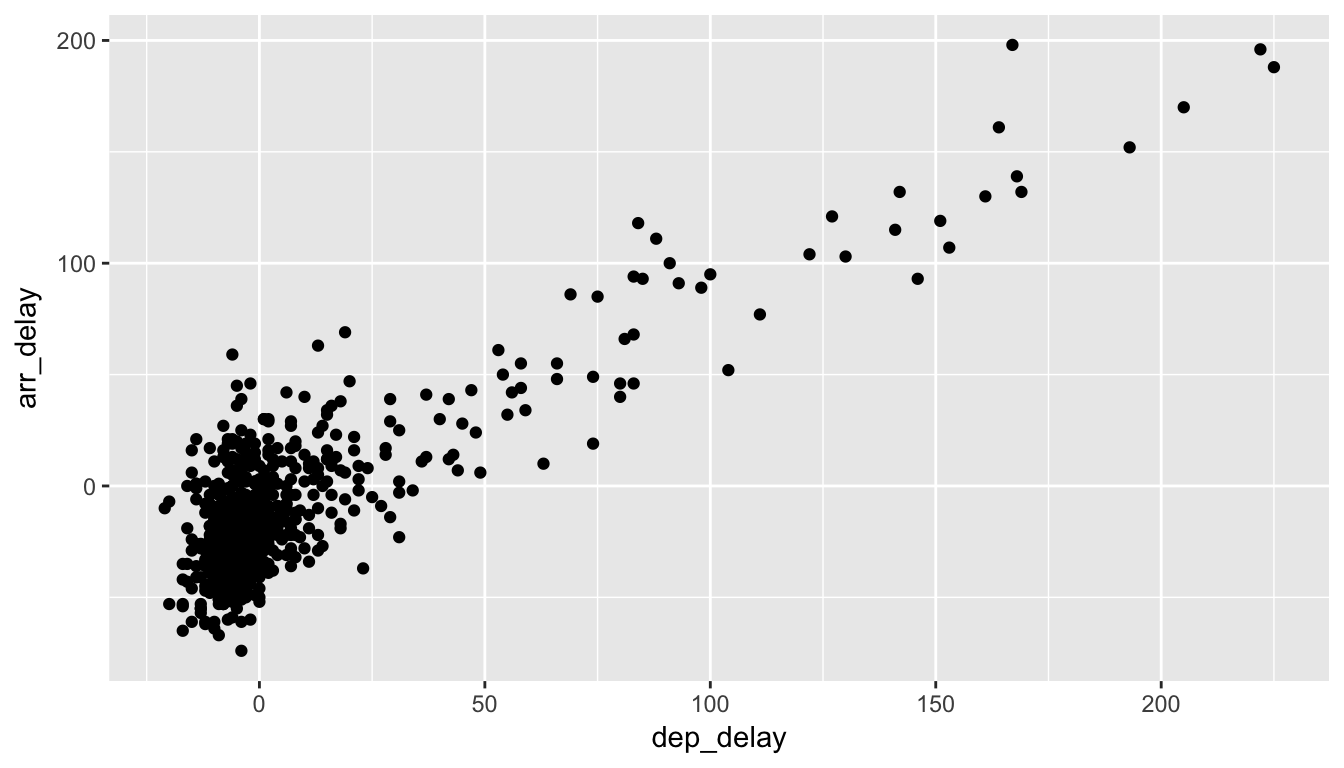
\includegraphics[width=\textwidth]{ismaykim_files/figure-latex/noalpha-1} 

}

\caption[Arrival Delays vs Departure Delays for Alaska Airlines flights from NYC in 2013]{Arrival Delays vs Departure Delays for Alaska Airlines flights from NYC in 2013}\label{fig:noalpha}
\end{figure}

You are encouraged to enter \textbf{Return} on your keyboard after
entering the \texttt{+}. As we add more and more elements, it will be
nice to keep them indented as you see below. Note that this will not
work if you begin the line with the \texttt{+}.

Let's break down this keeping in mind our discussion in Section
\ref{grammarofgraphics}:

\begin{itemize}
\tightlist
\item
  Within the \texttt{ggplot()} function call, we specify two of the
  components of the grammar:

  \begin{enumerate}
  \def\labelenumi{\arabic{enumi}.}
  \tightlist
  \item
    The \texttt{data} frame to be \texttt{all\_alaska\_flights} by
    setting \texttt{data\ =\ all\_alaska\_flights}
  \item
    The \texttt{aes}thetic mapping by setting
    \texttt{aes(x\ =\ dep\_delay,\ y\ =\ arr\_delay)}. Specifically

    \begin{itemize}
    \tightlist
    \item
      \texttt{dep\_delay} maps to the \texttt{x} position
    \item
      \texttt{arr\_delay} maps to the \texttt{y} position
    \end{itemize}
  \end{enumerate}
\item
  We add a \textbf{layer} to the \texttt{ggplot()} function call using
  the \texttt{+} sign
\item
  The layer in question specifies the third component of the grammar:
  the \texttt{geom}etric object in question. In this case the geometric
  object are \texttt{point}s, set by specifying \texttt{geom\_point()}
\end{itemize}

In Figure \ref{fig:noalpha} we see that a positive relationship exists
between \texttt{dep\_delay} and \texttt{arr\_delay}: as departure delays
increase, arrival delays tend to also increase. We also note that the
majority of points fall near the point (0, 0). There is a large mass of
points clustered there. (We will work more with this data set in Chapter
\ref{regress}, where we investigate correlation and linear regression.)

\begin{center}\rule{0.5\linewidth}{\linethickness}\end{center}

\begin{learncheck}
\textbf{\emph{Learning check}}
\end{learncheck}

\textbf{(LC4.2)} What are some practical reasons why \texttt{dep\_delay}
and \texttt{arr\_delay} have a positive relationship?

\textbf{(LC4.3)} What variables (not necessarily in the \texttt{flights}
data frame) would you expect to have a negative correlation (i.e.~a
negative relationship) with \texttt{dep\_delay}? Why? Remember that we
are focusing on continuous variables here.

\textbf{(LC4.4)} Why do you believe there is a cluster of points near
(0, 0)? What does (0, 0) correspond to in terms of the Alaskan flights?

\textbf{(LC4.5)} What are some other features of the plot that stand out
to you?

\textbf{(LC4.6)} Create a new scatter-plot using different variables in
the \texttt{all\_alaska\_flights} data frame by modifying the example
above.

\begin{center}\rule{0.5\linewidth}{\linethickness}\end{center}

\subsection{Over-Plotting}\label{over-plotting}

The large mass of points near (0, 0) can cause some confusion. This is
the result of a phenomenon called \textbf{over-plotting}. As one may
guess, this corresponds to values being plotted on top of each other
\emph{over} and \emph{over} again. It is often difficult to know just
how many values are plotted in this way when looking at a basic
scatter-plot as we have here. There are two ways to address this issue:

\begin{enumerate}
\def\labelenumi{\arabic{enumi}.}
\tightlist
\item
  By adjusting the transparency of the points via the \texttt{alpha}
  argument
\item
  By jittering the points via \texttt{geom\_jitter()}
\end{enumerate}

The first way of relieving over-plotting is by changing the
\texttt{alpha} argument to \texttt{geom\_point()} which controls the
transparency of the points. By default, this value is set to \texttt{1}.
We can change this value to a smaller fraction (greater than 0) to
change the transparency of the points in the plot:

\begin{Shaded}
\begin{Highlighting}[]
\KeywordTok{ggplot}\NormalTok{(}\DataTypeTok{data =} \NormalTok{all_alaska_flights, }\KeywordTok{aes}\NormalTok{(}\DataTypeTok{x =} \NormalTok{dep_delay, }\DataTypeTok{y =} \NormalTok{arr_delay)) +}\StringTok{ }
\StringTok{  }\KeywordTok{geom_point}\NormalTok{(}\DataTypeTok{alpha =} \FloatTok{0.2}\NormalTok{)}
\end{Highlighting}
\end{Shaded}

\begin{figure}

{\centering 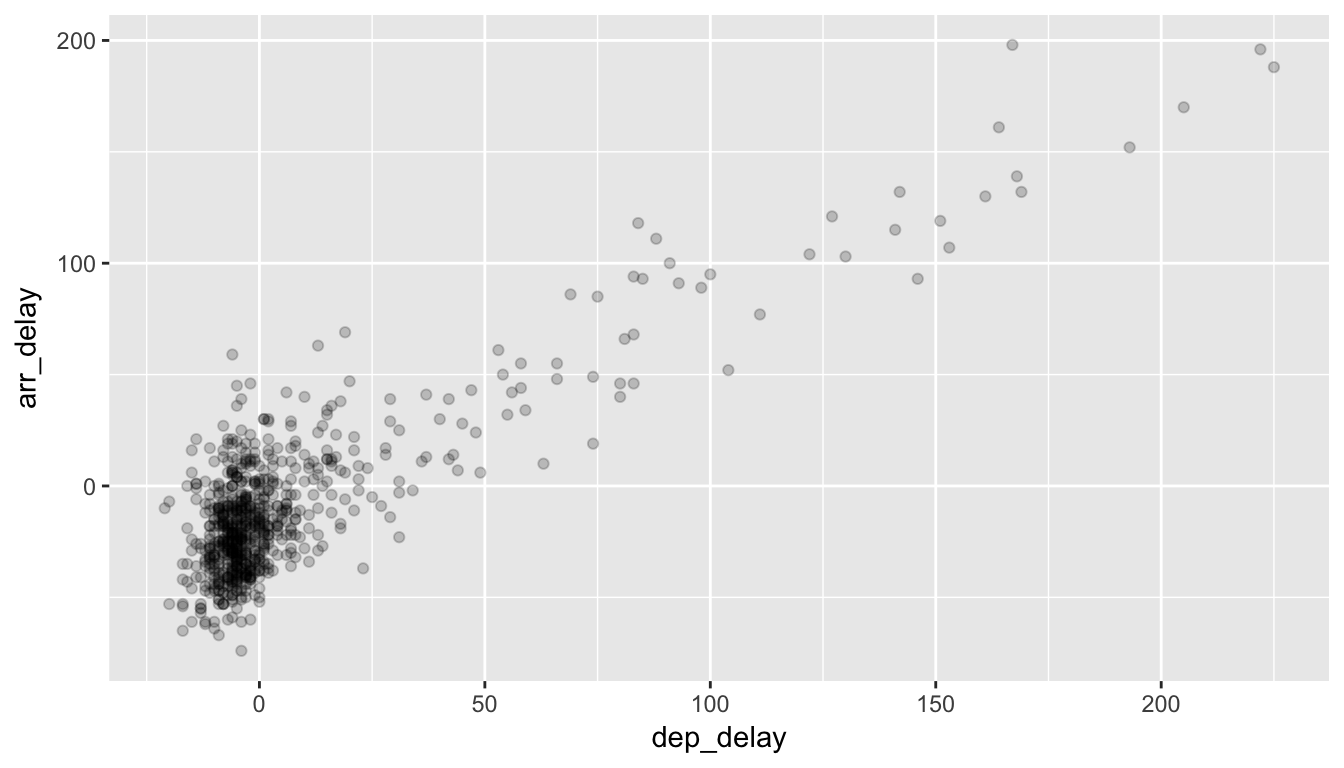
\includegraphics[width=\textwidth]{ismaykim_files/figure-latex/alpha-1} 

}

\caption[Delay scatterplot with alpha=0.2]{Delay scatterplot with alpha=0.2}\label{fig:alpha}
\end{figure}

Note how this function call is identical to the one in Section
\ref{scatterplots}, but with \texttt{geom\_point()} replaced with
\texttt{alpha\ =\ 0.2} added.

The second way of relieving over-plotting is to \textbf{jitter} the
points a bit. In other words, we are going to add just a bit of random
noise to the points to better see them and remove some of the
over-plotting. You can think of ``jittering'' as shaking the points a
bit on the plot. Instead of using \texttt{geom\_point}, we use
\texttt{geom\_jitter} to perform this shaking and specify around how
much jitter to add with the \texttt{width} and \texttt{height}
arguments. This corresponds to how hard you'd like to shake the plot in
units corresponding to those for both the horizontal and vertical
variables (in this case minutes).

\begin{Shaded}
\begin{Highlighting}[]
\KeywordTok{ggplot}\NormalTok{(}\DataTypeTok{data =} \NormalTok{all_alaska_flights, }\KeywordTok{aes}\NormalTok{(}\DataTypeTok{x =} \NormalTok{dep_delay, }\DataTypeTok{y =} \NormalTok{arr_delay)) +}\StringTok{ }
\StringTok{  }\KeywordTok{geom_jitter}\NormalTok{(}\DataTypeTok{width =} \DecValTok{30}\NormalTok{, }\DataTypeTok{height =} \DecValTok{30}\NormalTok{)}
\end{Highlighting}
\end{Shaded}

\begin{figure}

{\centering 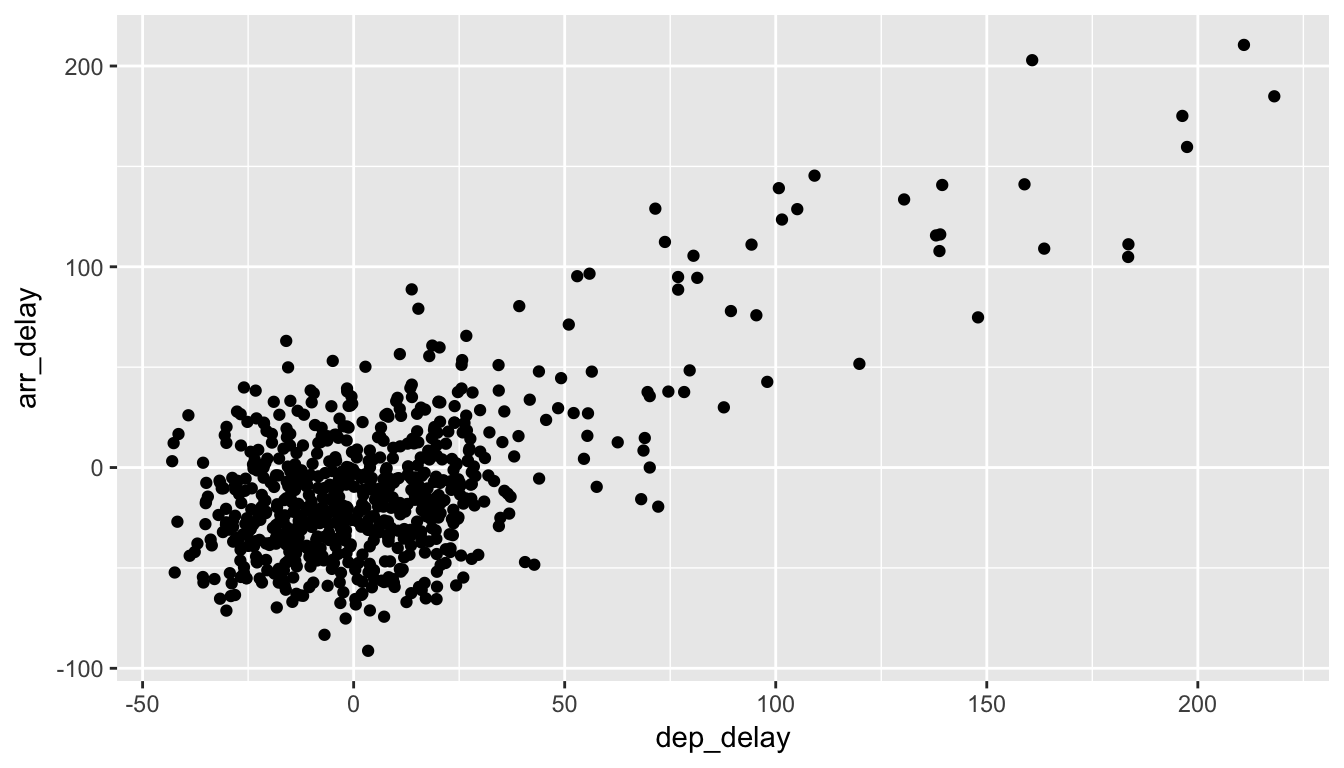
\includegraphics[width=\textwidth]{ismaykim_files/figure-latex/jitter-1} 

}

\caption[Jittered delay scatterplot]{Jittered delay scatterplot}\label{fig:jitter}
\end{figure}

Note how this function call is identical to the one in Section
\ref{geompoint}, but with \texttt{geom\_point()} replaced with
\texttt{geom\_jitter()}. The plot in \ref{fig:jitter} helps us a little
bit in getting a sense for the over-plotting, but with a relatively
large dataset like this one (714 flights), it can be argued that
changing the transparency of the points by setting \texttt{alpha} proved
more effective.

\begin{center}\rule{0.5\linewidth}{\linethickness}\end{center}

\begin{learncheck}
\textbf{\emph{Learning check}}
\end{learncheck}

\textbf{(LC4.7)} Why is setting the \texttt{alpha} argument value useful
with scatter-plots? What further information does it give you that a
regular scatter-plot cannot?

\textbf{(LC4.8)} After viewing the Figure \ref{fig:alpha} above, give a
range of arrival times and departure times that occur most frequently?
How has that region changed compared to when you observed the same plot
without the \texttt{alpha\ =\ 0.2} set in Figure \ref{fig:noalpha}?

\begin{center}\rule{0.5\linewidth}{\linethickness}\end{center}

\subsection{Summary}\label{summary}

Scatter-plots display the relationship between two continuous variables
and may be the most used plot today as they can provide an immediate way
to see the trend in one variable versus another. If you try to create a
scatter-plot where either one of the two variables is not quantitative
however, you will get strange results. Be careful!

With medium to large datasets, you may need to play with either
\texttt{geom\_jitter} or the \texttt{alpha} argument in order to get a
good feel for relationships in your data. This tweaking is often a fun
part of data visualization since you'll have the chance to see different
relationships come about as you make subtle changes to your plots.

\section{5NG\#2: Line-graphs}\label{linegraphs}

The next of the 5NG is a line-graph. They are most frequently used when
the x-axis represents time and the y-axis represents some other
numerical variable; such plots are known as \textbf{time series}. Time
represents a variable that is connected together by each day following
the previous day. In other words, time has a natural ordering.
Line-graphs should be avoided when there is not a clear sequential
ordering to the explanatory variable, i.e.~the x-variable or the
\emph{predictor} variable.

Our focus turns to the \texttt{temp} variable in this \texttt{weather}
dataset. By

\begin{itemize}
\tightlist
\item
  Looking over the \texttt{weather} dataset by typing
  \texttt{View(weather)} in the console.
\item
  Running \texttt{?weather} to bring up the help file.
\end{itemize}

We can see that the \texttt{temp} variable corresponds to hourly
temperature (in Fahrenheit) recordings at weather stations near airports
in New York City. Instead of considering all hours in 2013 for all three
airports in NYC, let's focus on the hourly temperature at Newark airport
(\texttt{origin} code ``EWR'') for the first 15 days in January 2013.
The \texttt{weather} data frame in the \texttt{nycflights13} package
contains this data, but we first need to filter it to only include those
rows that correspond to Newark in the first 15 days of January.

\begin{Shaded}
\begin{Highlighting}[]
\KeywordTok{data}\NormalTok{(weather)}
\NormalTok{early_january_weather <-}\StringTok{ }\NormalTok{weather %>%}\StringTok{ }
\StringTok{  }\KeywordTok{filter}\NormalTok{(origin ==}\StringTok{ "EWR"} \NormalTok{&}\StringTok{ }\NormalTok{month ==}\StringTok{ }\DecValTok{1} \NormalTok{&}\StringTok{ }\NormalTok{day <=}\StringTok{ }\DecValTok{15}\NormalTok{)}
\end{Highlighting}
\end{Shaded}

This is similar to the previous use of the \texttt{filter} command in
Section \ref{scatterplots}, however we now use the \texttt{\&} operator.
The above selects only those rows in \texttt{weather} where
\texttt{origin\ ==\ "EWR"} \textbf{and} \texttt{month\ =\ 1}
\textbf{and} \texttt{day\ \textless{}=\ 15}.

\begin{center}\rule{0.5\linewidth}{\linethickness}\end{center}

\begin{learncheck}
\textbf{\emph{Learning check}}
\end{learncheck}

\textbf{(LC4.9)} Take a look at both the \texttt{weather} and
\texttt{early\_january\_weather} data frames by running
\texttt{View(weather)} and \texttt{View(early\_january\_weather)} in the
console. In what respect do these data frames differ?

\textbf{(LC4.10)} The weather data is recorded hourly. Why does the
\texttt{time\_hour} variable correctly identify the hour of the
measurement whereas the \texttt{hour} variable does not?

\begin{center}\rule{0.5\linewidth}{\linethickness}\end{center}

\subsection{Line-graphs via geom\_line}\label{geomline}

We plot a line-graph of hourly temperature using \texttt{geom\_line()}:

\begin{Shaded}
\begin{Highlighting}[]
\KeywordTok{ggplot}\NormalTok{(}\DataTypeTok{data =} \NormalTok{early_january_weather, }\KeywordTok{aes}\NormalTok{(}\DataTypeTok{x =} \NormalTok{time_hour, }\DataTypeTok{y =} \NormalTok{temp)) +}
\StringTok{  }\KeywordTok{geom_line}\NormalTok{()}
\end{Highlighting}
\end{Shaded}

\begin{figure}

{\centering 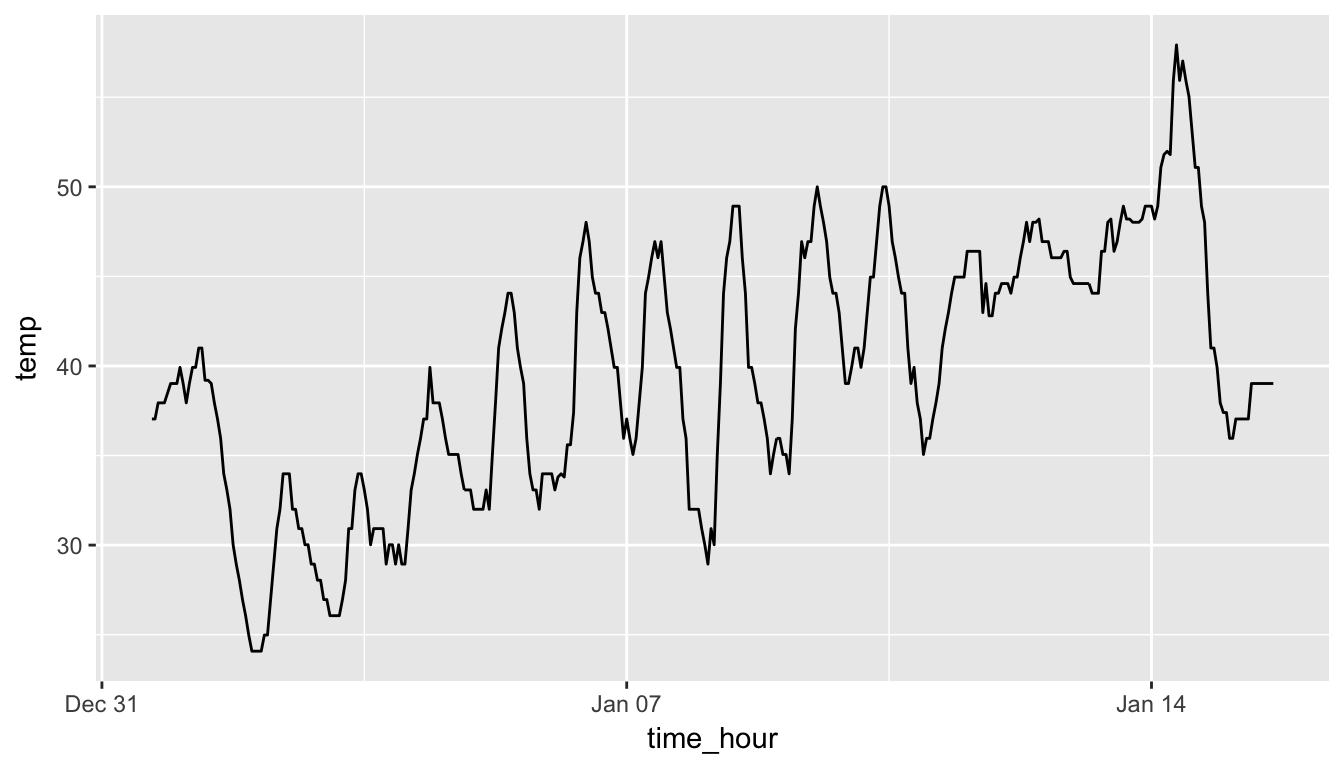
\includegraphics[width=\textwidth]{ismaykim_files/figure-latex/hourlytemp-1} 

}

\caption[Hourly Temperature in Newark for Jan 1-15 2013]{Hourly Temperature in Newark for Jan 1-15 2013}\label{fig:hourlytemp}
\end{figure}

Much as with the \texttt{ggplot()} call in Section \ref{geompoint}, we
specify the components of the Grammar of Graphics:

\begin{itemize}
\tightlist
\item
  Within the \texttt{ggplot()} function call, we specify two of the
  components of the grammar:

  \begin{enumerate}
  \def\labelenumi{\arabic{enumi}.}
  \tightlist
  \item
    The \texttt{data} frame to be \texttt{early\_january\_weather} by
    setting \texttt{data\ =\ early\_january\_weather}
  \item
    The \texttt{aes}thetic mapping by setting
    \texttt{aes(x\ =\ time\_hour,\ y\ =\ temp)}. Specifically

    \begin{itemize}
    \tightlist
    \item
      \texttt{time\_hour} (i.e.~the time variable) maps to the
      \texttt{x} position
    \item
      \texttt{temp} maps to the \texttt{y} position
    \end{itemize}
  \end{enumerate}
\item
  We add a \textbf{layer} to the \texttt{ggplot()} function call using
  the \texttt{+} sign
\item
  The layer in question specifies the third component of the grammar:
  the \texttt{geom}etric object in question. In this case the geometric
  object is a \texttt{line}, set by specifying \texttt{geom\_line()}
\end{itemize}

\begin{center}\rule{0.5\linewidth}{\linethickness}\end{center}

\begin{learncheck}
\textbf{\emph{Learning check}}
\end{learncheck}

\textbf{(LC4.11)} Why should line-graphs be avoided when there is not a
clear ordering of the horizontal axis?

\textbf{(LC4.12)} Why are line-graphs frequently used when time is the
explanatory variable?

\textbf{(LC4.13)} Plot a time series of a variable other than
\texttt{temp} for Newark Airport in the first 15 days of January 2013.

\begin{center}\rule{0.5\linewidth}{\linethickness}\end{center}

\subsection{Summary}\label{summary-1}

Line-graphs, just like scatter-plots, display the relationship between
two continuous variables. However the variable on the x-axis (i.e.~the
explanatory variable) should have a natural ordering, like some notion
of time. We can mislead our audience if that isn't the case.

\section{5NG\#3: Histograms}\label{histograms}

Let's consider the \texttt{temp} variable in the \texttt{weather} data
frame once again, but now unlike with the line-graphs in Section
\ref{linegraphs}, let's say we don't care about the relationship of
temperature to time, but rather you care about the \textbf{(statistical)
distribution} of temperatures. We could just produce points where each
of the different values appear on something similar to a number line:

\begin{figure}

{\centering 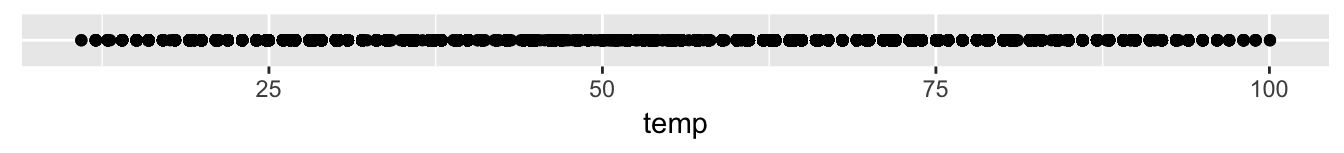
\includegraphics[width=\textwidth]{ismaykim_files/figure-latex/unnamed-chunk-20-1} 

}

\caption[Strip Plot of Hourly Temperature Recordings from NYC in 2013]{Strip Plot of Hourly Temperature Recordings from NYC in 2013}\label{fig:unnamed-chunk-20}
\end{figure}

This gives us a general idea of how the values of \texttt{temp} differ.
We see that temperatures vary from around 11 up to 100 degrees
Fahrenheit. The area between 40 and 60 degrees appears to have more
points plotted than outside that range.

\subsection{Histograms via geom\_histogram}\label{geomhistogram}

What is commonly produced instead of this strip plot is a plot known as
a \textbf{histogram}. The \textbf{histogram} shows how many elements of
a single numerical variable fall in specified \textbf{bins}. In this
case, these \textbf{bins} may correspond to between 0-10°F, 10-20°F,
etc. We produce a histogram of the hour temperatures at all three NYC
airports in 2013:

\begin{Shaded}
\begin{Highlighting}[]
\KeywordTok{ggplot}\NormalTok{(}\DataTypeTok{data =} \NormalTok{weather, }\DataTypeTok{mapping =} \KeywordTok{aes}\NormalTok{(}\DataTypeTok{x =} \NormalTok{temp)) +}
\StringTok{  }\KeywordTok{geom_histogram}\NormalTok{()}
\end{Highlighting}
\end{Shaded}

\begin{verbatim}
## `stat_bin()` using `bins = 30`. Pick better value with `binwidth`.
\end{verbatim}

\begin{verbatim}
## Warning: Removed 1 rows containing non-finite values (stat_bin).
\end{verbatim}

\begin{figure}

{\centering 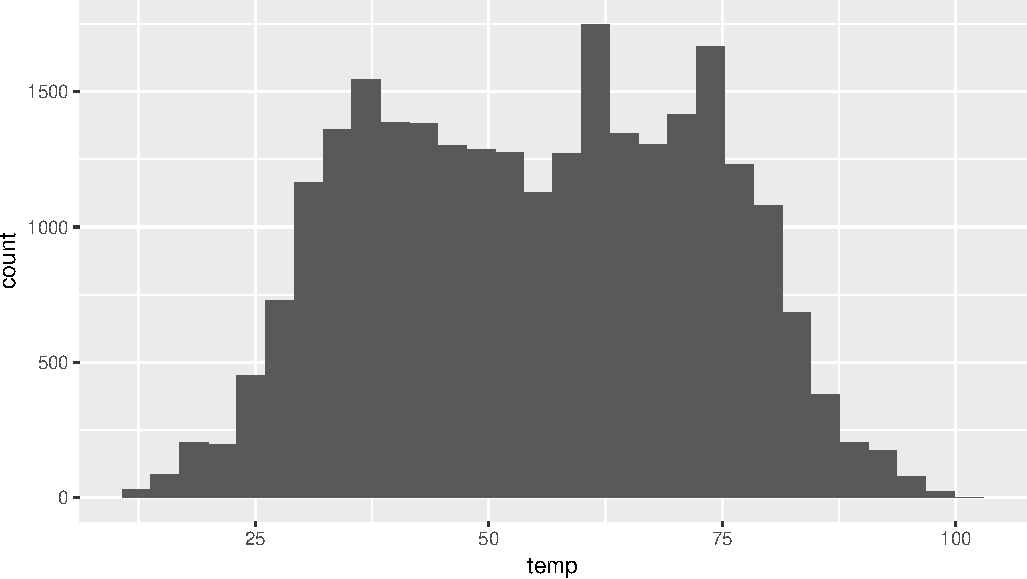
\includegraphics[width=\textwidth]{ismaykim_files/figure-latex/unnamed-chunk-21-1} 

}

\caption[Histogram of Hourly Temperature Recordings from NYC in 2013]{Histogram of Hourly Temperature Recordings from NYC in 2013}\label{fig:unnamed-chunk-21}
\end{figure}

Note here:

\begin{itemize}
\tightlist
\item
  There is only one variable being mapped in \texttt{aes()}: the single
  continuous variable \texttt{temp}. You don't need to compute the
  y-aesthetic: it gets computed automatically.
\item
  We set the \texttt{geom}etric object to be \texttt{geom\_histogram()}
\item
  We got a warning message of
  \texttt{1\ rows\ containing\ non-finite\ values} being removed. This
  is due to one of the values of temperature being missing. R is
  alerting us that this happened.
\end{itemize}

\subsection{Adjusting the Bins}\label{adjustbins}

We can adjust the number/size of the bins two ways:

\begin{enumerate}
\def\labelenumi{\arabic{enumi}.}
\tightlist
\item
  By adjusting the number of bins via the \texttt{bins} argument
\item
  By adjusting the width of the bins via the \texttt{binwidth} argument
\end{enumerate}

First, we have the power to specify how many bins we would like to put
the data into as an argument in the \texttt{geom\_histogram} function.
By default, this is chosen to be 30 somewhat arbitrarily; we have
received a warning above our plot that this was done.

\begin{Shaded}
\begin{Highlighting}[]
\KeywordTok{ggplot}\NormalTok{(}\DataTypeTok{data =} \NormalTok{weather, }\DataTypeTok{mapping =} \KeywordTok{aes}\NormalTok{(}\DataTypeTok{x =} \NormalTok{temp)) +}
\StringTok{  }\KeywordTok{geom_histogram}\NormalTok{(}\DataTypeTok{bins =} \DecValTok{60}\NormalTok{, }\DataTypeTok{color =} \StringTok{"white"}\NormalTok{)}
\end{Highlighting}
\end{Shaded}

\begin{figure}

{\centering 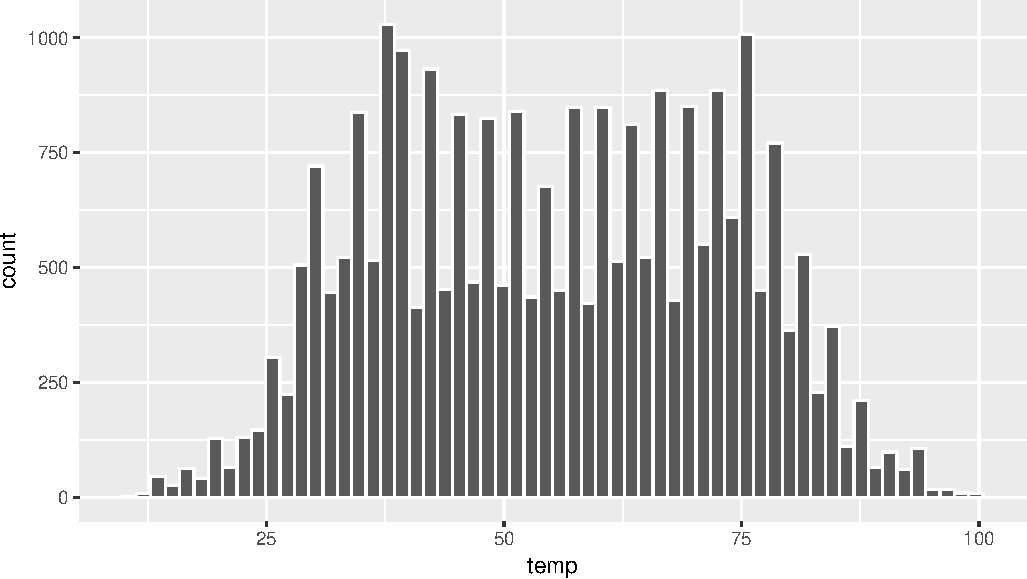
\includegraphics[width=\textwidth]{ismaykim_files/figure-latex/unnamed-chunk-22-1} 

}

\caption[Histogram of Hourly Temperature Recordings from NYC in 2013 - 60 Bins]{Histogram of Hourly Temperature Recordings from NYC in 2013 - 60 Bins}\label{fig:unnamed-chunk-22}
\end{figure}

Note the addition of the \texttt{color} argument. If you'd like to be
able to more easily differentiate each of the bins, you can specify the
color of the outline as done above.

Second, instead of specifying the number of bins, we can also specify
the width of the bins by using the \texttt{binwidth} argument in the
\texttt{geom\_histogram} function.

\begin{Shaded}
\begin{Highlighting}[]
\KeywordTok{ggplot}\NormalTok{(}\DataTypeTok{data =} \NormalTok{weather, }\DataTypeTok{mapping =} \KeywordTok{aes}\NormalTok{(}\DataTypeTok{x =} \NormalTok{temp)) +}
\StringTok{  }\KeywordTok{geom_histogram}\NormalTok{(}\DataTypeTok{binwidth =} \DecValTok{10}\NormalTok{, }\DataTypeTok{color =} \StringTok{"white"}\NormalTok{)}
\end{Highlighting}
\end{Shaded}

\begin{figure}

{\centering 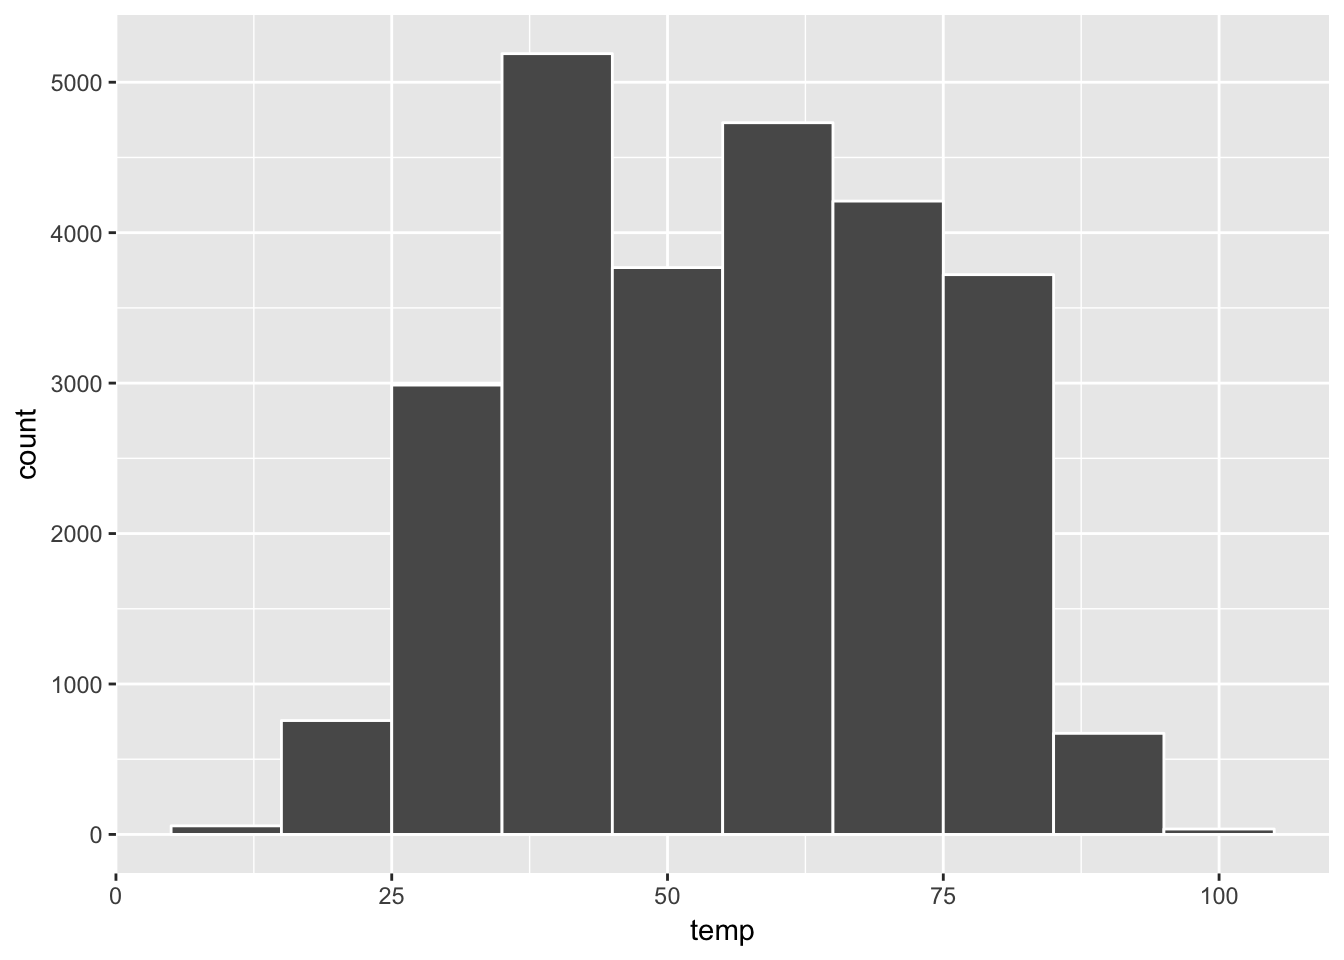
\includegraphics[width=\textwidth]{ismaykim_files/figure-latex/unnamed-chunk-23-1} 

}

\caption[Histogram of Hourly Temperature Recordings from NYC in 2013 - Binwidth = 10]{Histogram of Hourly Temperature Recordings from NYC in 2013 - Binwidth = 10}\label{fig:unnamed-chunk-23}
\end{figure}

\begin{center}\rule{0.5\linewidth}{\linethickness}\end{center}

\begin{learncheck}
\textbf{\emph{Learning check}}
\end{learncheck}

\textbf{(LC4.14)} What does changing the number of bins from 30 to 60
tell us about the distribution of temperatures?

\textbf{(LC4.15)} Would you classify the distribution of temperatures as
symmetric or skewed?

\textbf{(LC4.16)} What would you guess is the ``center'' value in this
distribution? Why did you make that choice?

\textbf{(LC4.17)} Is this data spread out greatly from the center or is
it close? Why?

\begin{center}\rule{0.5\linewidth}{\linethickness}\end{center}

\subsection{Summary}\label{summary-2}

Histograms, unlike scatter-plots and line-graphs, presents information
on only a single continuous variable. In particular they are
visualizations of the (statistical) distribution of values.

\section{Facets}\label{facets}

Before continuing the 5NG, we briefly introduce a new concept called
\textbf{faceting}. Faceting is used when we'd like to create small
multiples of the same plot over a different categorical variable. By
default, all of the small multiples will have the same vertical axis.

For example, suppose we were interested in looking at how the
temperature histograms we saw in Section \ref{histograms} varied by
month. This is what is meant by ``the distribution of a variable over
another variable'': \texttt{temp} is one variable and \texttt{month} is
the other variable. In order to look at histograms of \texttt{temp} for
each month, we add a layer \texttt{facet\_wrap(\textasciitilde{}month)}.
You can also specify how many rows you'd like the small multiple plots
to be in using \texttt{nrow} inside of \texttt{facet\_wrap}.

\begin{Shaded}
\begin{Highlighting}[]
\KeywordTok{ggplot}\NormalTok{(}\DataTypeTok{data =} \NormalTok{weather, }\KeywordTok{aes}\NormalTok{(}\DataTypeTok{x =} \NormalTok{temp)) +}
\StringTok{  }\KeywordTok{geom_histogram}\NormalTok{(}\DataTypeTok{binwidth =} \DecValTok{5}\NormalTok{, }\DataTypeTok{color =} \StringTok{"white"}\NormalTok{) +}
\StringTok{  }\KeywordTok{facet_wrap}\NormalTok{(~}\StringTok{ }\NormalTok{month, }\DataTypeTok{nrow =} \DecValTok{4}\NormalTok{)}
\end{Highlighting}
\end{Shaded}

\begin{figure}

{\centering 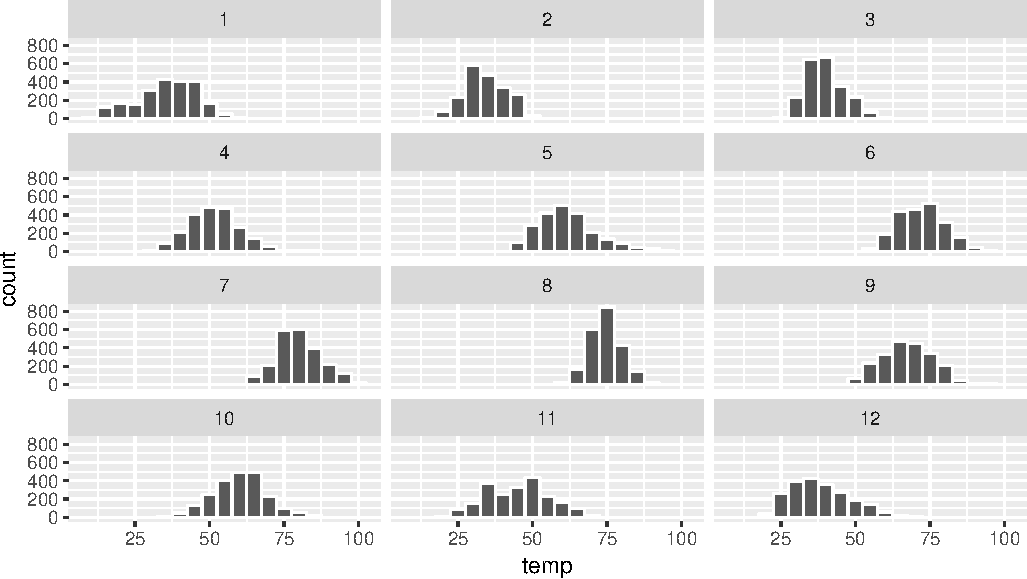
\includegraphics[width=\textwidth]{ismaykim_files/figure-latex/facethistogram-1} 

}

\caption[Faceted histogram]{Faceted histogram}\label{fig:facethistogram}
\end{figure}

As we might expect, the temperature tends to increase as summer
approaches and then decrease as winter approaches.

\begin{center}\rule{0.5\linewidth}{\linethickness}\end{center}

\begin{learncheck}
\textbf{\emph{Learning check}}
\end{learncheck}

\textbf{(LC4.18)} What other things do you notice about the faceted plot
above? How does a faceted plot help us see relationships between two
variables?

\textbf{(LC4.19)} What do the numbers 1-12 correspond to in the plot
above? What about 25, 50, 75, 100?

\textbf{(LC4.20)} For which types of datasets would these types of
faceted plots not work well in comparing relationships between
variables? Give an example describing the variability of the variables
and other important characteristics.

\textbf{(LC4.21)} Does the \texttt{temp} variable in the
\texttt{weather} data set have a lot of variability? Why do you say
that?

\begin{center}\rule{0.5\linewidth}{\linethickness}\end{center}

\section{5NG\#4: Boxplots}\label{ng4-boxplots}

While using faceted histograms can provide a way to compare
distributions of a continuous variable split by groups of a categorical
variable as in Chapter \ref{facets}, an alternative plot called a
\textbf{boxplot} (also called a \textbf{side-by-side boxplot}) achieves
the same task and is frequently preferred. The \textbf{boxplot} uses the
information provided in the \textbf{five-number summary} referred to in
Appendix \ref{appendixA}. It gives a way to compare this summary
information across the different levels of a categorical variable.

\subsection{Boxplots via geom\_boxplot}\label{geomboxplot}

Let's create a boxplot to compare the monthly temperatures as we did
above with the faceted histograms.

\begin{Shaded}
\begin{Highlighting}[]
\KeywordTok{ggplot}\NormalTok{(}\DataTypeTok{data =} \NormalTok{weather, }\KeywordTok{aes}\NormalTok{(}\DataTypeTok{x =} \NormalTok{month, }\DataTypeTok{y =} \NormalTok{temp)) +}
\StringTok{  }\KeywordTok{geom_boxplot}\NormalTok{()}
\end{Highlighting}
\end{Shaded}

\begin{figure}

{\centering 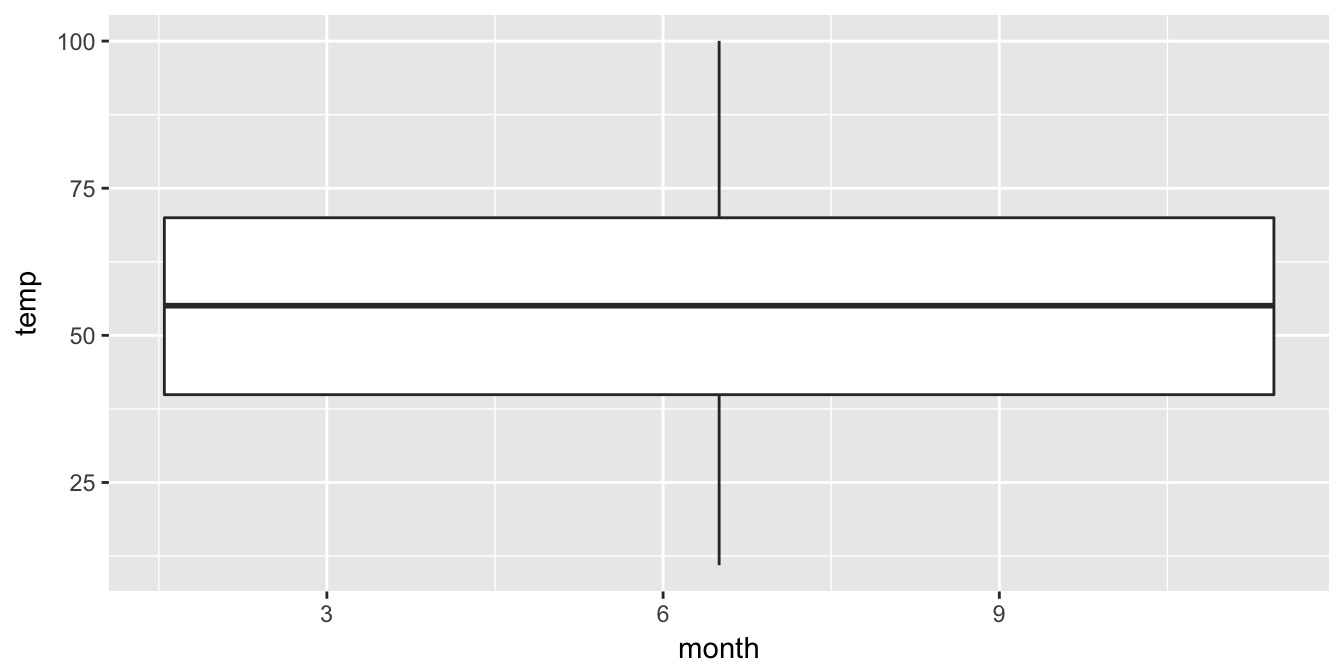
\includegraphics[width=\textwidth]{ismaykim_files/figure-latex/badbox-1} 

}

\caption[Invalid boxplot specification]{Invalid boxplot specification}\label{fig:badbox}
\end{figure}

Note the first warning that is given here. (The second one corresponds
to missing values in the data frame and it is turned off on subsequent
plots.) Observe that this plot does not look like what we were
expecting. We were expecting to see the distribution of temperatures for
each month (so 12 different boxplots). This gives us the overall boxplot
without any other groupings. We can get around this by introducing a new
function for our \texttt{x} variable:

\begin{Shaded}
\begin{Highlighting}[]
\KeywordTok{ggplot}\NormalTok{(}\DataTypeTok{data =} \NormalTok{weather, }\DataTypeTok{mapping =} \KeywordTok{aes}\NormalTok{(}\DataTypeTok{x =} \KeywordTok{factor}\NormalTok{(month), }\DataTypeTok{y =} \NormalTok{temp)) +}
\StringTok{  }\KeywordTok{geom_boxplot}\NormalTok{()}
\end{Highlighting}
\end{Shaded}

\begin{figure}

{\centering 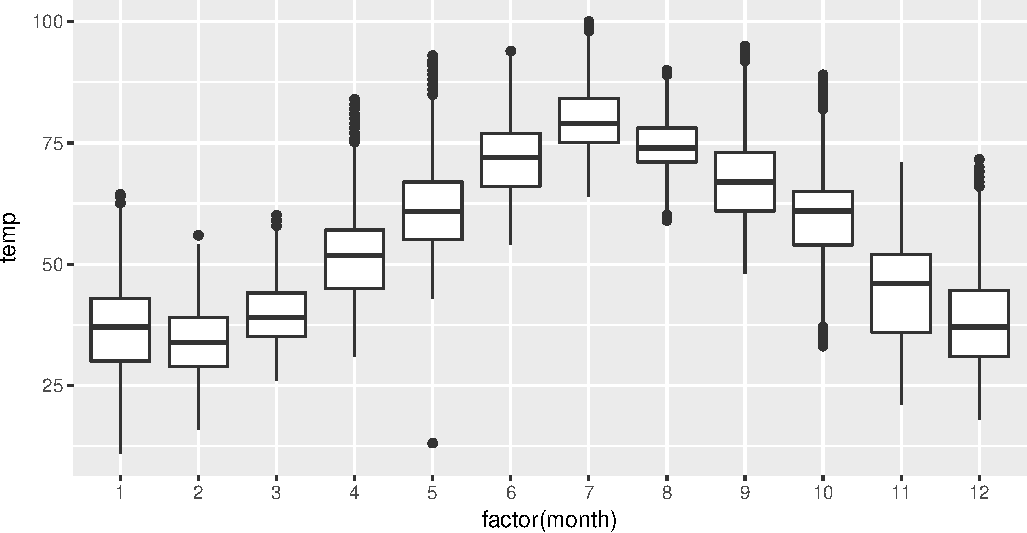
\includegraphics[width=\textwidth]{ismaykim_files/figure-latex/monthtempbox-1} 

}

\caption[Month by temp boxplot]{Month by temp boxplot}\label{fig:monthtempbox}
\end{figure}

We have introduced a new function called \texttt{factor()} here. One of
the things this function does is to convert a discrete value like
\texttt{month} (1, 2, \ldots{}, 12) into a categorical variable. The
``box'' part of this plot represents the 25\textsuperscript{th}
percentile, the median (50\textsuperscript{th} percentile), and the
75\textsuperscript{th} percentile. The dots correspond to
\textbf{outliers}. (The specific formulation for these outliers is
discussed in Appendix \ref{appendixA}.) The lines show how the data
varies that is not in the center 50\% defined by the first and third
quantiles. Longer lines correspond to more variability and shorter lines
correspond to less variability.

\begin{center}\rule{0.5\linewidth}{\linethickness}\end{center}

\begin{learncheck}
\textbf{\emph{Learning check}}
\end{learncheck}

\textbf{(LC4.22)} What does the dot at the bottom of the plot for May
correspond to? Explain what might have occurred in May to produce this
point.

\textbf{(LC4.23)} Which months have the highest variability in
temperature? What reasons do you think this is?

\textbf{(LC4.24)} We looked at the distribution of a continuous variable
over a categorical variable here with this boxplot. Why can't we look at
the distribution of one continuous variable over the distribution of
another continuous variable? Say, temperature across pressure, for
example?

\textbf{(LC4.25)} Boxplots provide a simple way to identify outliers.
Why may outliers be easier to identify when looking at a boxplot instead
of a faceted histogram?

\begin{center}\rule{0.5\linewidth}{\linethickness}\end{center}

\subsection{Summary}\label{summary-3}

Boxplots provide a way to compare and contrast the distribution of one
quantitative variable across multiple levels of one categorical
variable. One can easily look to see where the median falls across the
different groups by looking at the center line in the box. You can also
see how spread out the variable is across the different groups by
looking at the width of the box and also how far out the lines stretch
from the box. If the lines stretch far from the box but the box has a
small width, the variability of the values closer to the center is much
smaller than the variability of the outer ends of the variable. Lastly,
outliers are even more easily identified when looking at a boxplot than
when looking at a histogram.

\section{5NG\#5: Barplots}\label{geombar}

Both histograms and boxplots represent ways to visualize the variability
of continuous variables. Another common task is to present the
distribution of a categorical variable. This is a simpler task since we
will be interested in how many elements from our data fall into the
different categories of the categorical variable.

\subsection{Barplots via geom\_bar}\label{barplots-via-geom_bar}

Frequently, the best way to visualize these different counts (also known
as \textbf{frequencies}) is via a barplot. Consider the distribution of
airlines that flew out of New York City in 2013. Here we explore the
number of flights from each airline/\texttt{carrier}. This can be
plotted by invoking the \texttt{geom\_bar} function in \texttt{ggplot2}:

\begin{Shaded}
\begin{Highlighting}[]
\KeywordTok{ggplot}\NormalTok{(}\DataTypeTok{data =} \NormalTok{flights, }\DataTypeTok{mapping =} \KeywordTok{aes}\NormalTok{(}\DataTypeTok{x =} \NormalTok{carrier)) +}
\StringTok{  }\KeywordTok{geom_bar}\NormalTok{()}
\end{Highlighting}
\end{Shaded}

\begin{figure}

{\centering 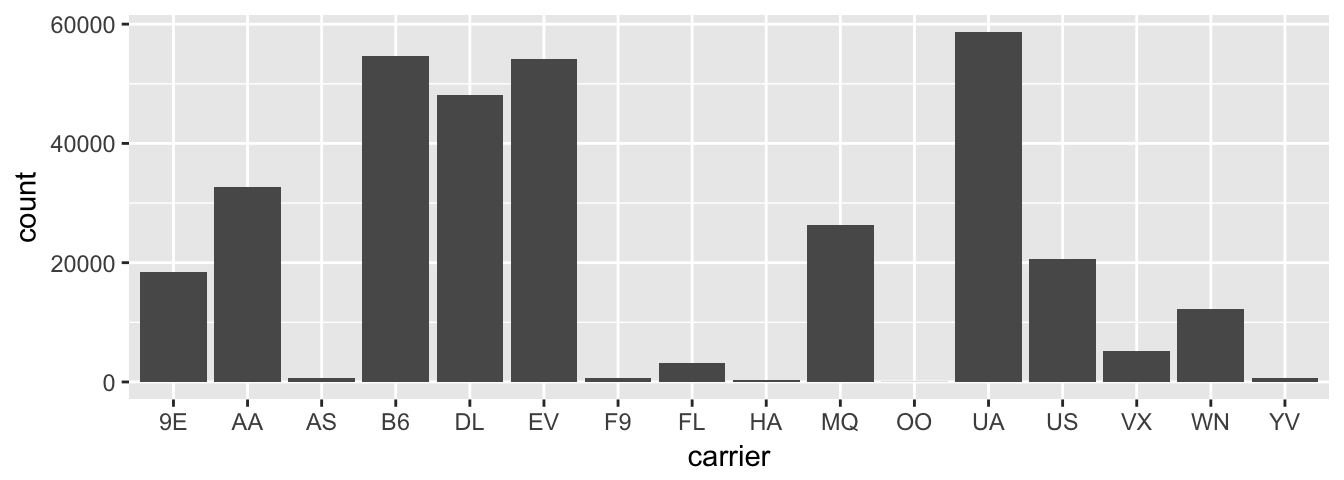
\includegraphics[width=\textwidth]{ismaykim_files/figure-latex/flightsbar-1} 

}

\caption[Number of flights departing NYC in 2013 by airline]{Number of flights departing NYC in 2013 by airline}\label{fig:flightsbar}
\end{figure}

To get an understanding of what the names of these airlines are
corresponding to these \texttt{carrier} codes, we can look at the
\texttt{airlines} data frame in the \texttt{nycflights13} package. Note
the use of the \texttt{kable} function here in the \texttt{knitr}
package, which produces a nicely-formatted table of the values in the
\texttt{airlines} data frame.

\begin{Shaded}
\begin{Highlighting}[]
\KeywordTok{data}\NormalTok{(airlines)}
\KeywordTok{kable}\NormalTok{(airlines)}
\end{Highlighting}
\end{Shaded}

\begin{tabular}{l|l}
\hline
carrier & name\\
\hline
9E & Endeavor Air Inc.\\
\hline
AA & American Airlines Inc.\\
\hline
AS & Alaska Airlines Inc.\\
\hline
B6 & JetBlue Airways\\
\hline
DL & Delta Air Lines Inc.\\
\hline
EV & ExpressJet Airlines Inc.\\
\hline
F9 & Frontier Airlines Inc.\\
\hline
FL & AirTran Airways Corporation\\
\hline
HA & Hawaiian Airlines Inc.\\
\hline
MQ & Envoy Air\\
\hline
OO & SkyWest Airlines Inc.\\
\hline
UA & United Air Lines Inc.\\
\hline
US & US Airways Inc.\\
\hline
VX & Virgin America\\
\hline
WN & Southwest Airlines Co.\\
\hline
YV & Mesa Airlines Inc.\\
\hline
\end{tabular}

Going back to our barplot, we see that United Air Lines, JetBlue
Airways, and ExpressJet Airlines had the most flights depart New York
City in 2013. To get the actual number of flights by each airline we can
use the \texttt{count} function in the \texttt{dplyr} package on the
\texttt{carrier} variable in \texttt{flights}, which we will introduce
formally in Chapter \ref{manip}.

\begin{Shaded}
\begin{Highlighting}[]
\NormalTok{flights_table <-}\StringTok{ }\NormalTok{flights %>%}\StringTok{ }\NormalTok{dplyr::}\KeywordTok{count}\NormalTok{(carrier)}
\NormalTok{knitr::}\KeywordTok{kable}\NormalTok{(flights_table)}
\end{Highlighting}
\end{Shaded}

\begin{tabular}{l|r}
\hline
carrier & n\\
\hline
9E & 18460\\
\hline
AA & 32729\\
\hline
AS & 714\\
\hline
B6 & 54635\\
\hline
DL & 48110\\
\hline
EV & 54173\\
\hline
F9 & 685\\
\hline
FL & 3260\\
\hline
HA & 342\\
\hline
MQ & 26397\\
\hline
OO & 32\\
\hline
UA & 58665\\
\hline
US & 20536\\
\hline
VX & 5162\\
\hline
WN & 12275\\
\hline
YV & 601\\
\hline
\end{tabular}

\textbf{Technical note}: Refer to the use of \texttt{::} in both lines
of code above. This is another way of ensuring the correct function is
called. A \texttt{count} exists in a couple different packages and
sometimes you'll receive strange errors when a different instance of a
function is used. This is a great way of telling R that ``I want this
one!''. You specify the name of the package directly before the
\texttt{::} and then the name of the function immediately after
\texttt{::}.

\begin{center}\rule{0.5\linewidth}{\linethickness}\end{center}

\begin{learncheck}
\textbf{\emph{Learning check}}
\end{learncheck}

\textbf{(LC4.26)} Why are histograms inappropriate for visualizing
categorical variables?

\textbf{(LC4.27)} What is the difference between histograms and
barplots?

\textbf{(LC4.28)} How many Envoy Air flights departed NYC in 2013?

\textbf{(LC4.29)} What was the seventh highest airline in terms of
departed flights from NYC in 2013? How could we better present the table
to get this answer quickly.

\begin{center}\rule{0.5\linewidth}{\linethickness}\end{center}

\subsection{Must avoid pie charts!}\label{must-avoid-pie-charts}

Unfortunately, one of the most common plots seen today for categorical
data is the pie chart. While they may see harmless enough, they actually
present a problem in that humans are unable to judge angles well. As
Naomi Robbins describes in her book ``Creating More Effective Graphs''
\citep{robbins2013}, we overestimate angles greater than 90 degrees and
we underestimate angles less than 90 degrees. In other words, it is
difficult for us to determine relative size of one piece of the pie
compared to another.

Let's examine our previous barplot example on the number of flights
departing NYC by airline. This time we will use a pie chart. As you
review this chart, try to identify

\begin{itemize}
\tightlist
\item
  how much larger the portion of the pie is for ExpressJet Airlines
  (\texttt{EV}) compared to US Airways (\texttt{US}),
\item
  what the third largest carrier is in terms of departing flights, and
\item
  how many carriers have fewer flights than United Airlines
  (\texttt{UA})?
\end{itemize}

\begin{figure}

{\centering 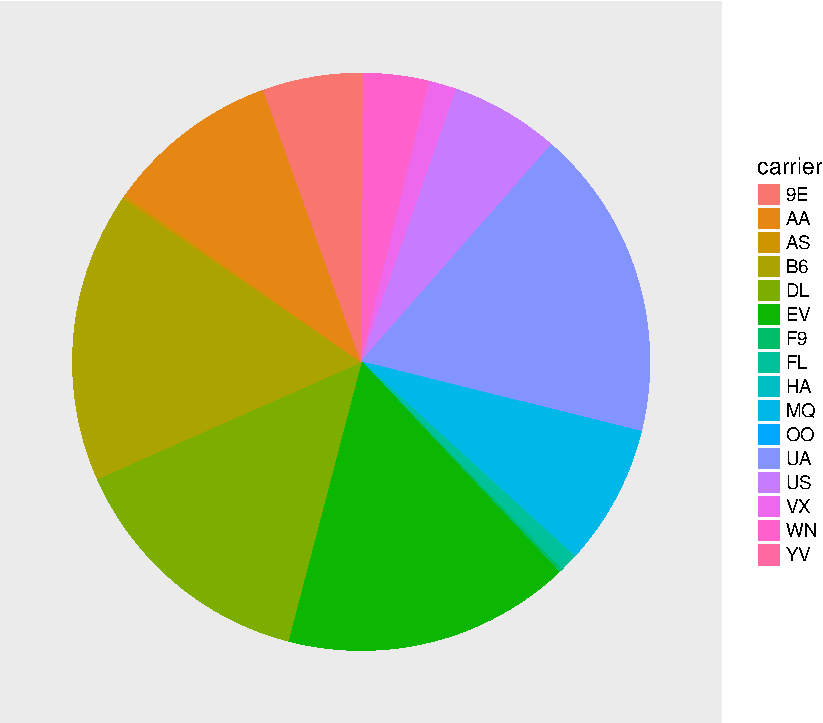
\includegraphics[width=\textwidth]{ismaykim_files/figure-latex/carrierpie-1} 

}

\caption[The dreaded pie chart]{The dreaded pie chart}\label{fig:carrierpie}
\end{figure}

While it is quite easy to look back at the barplot to get the answer to
these questions, it's quite difficult to get the answers correct when
looking at the pie graph. Barplots can always present the information in
a way that is easier for the eye to determine relative position. There
may be one exception from Nathan Yau at
\href{https://flowingdata.com/2008/09/19/pie-i-have-eaten-and-pie-i-have-not-eaten/}{FlowingData.com}
but we will leave this for the reader to decide:

\begin{figure}

{\centering 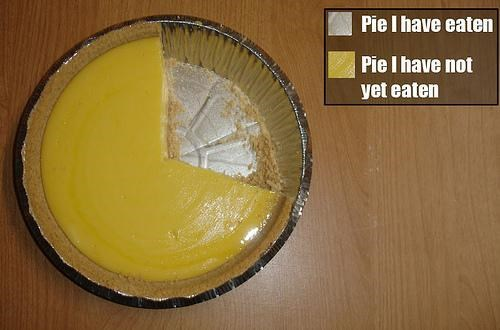
\includegraphics[width=\textwidth,height=2.5in]{images/Pie-I-have-Eaten} 

}

\caption[The only good pie chart]{The only good pie chart}\label{fig:unnamed-chunk-26}
\end{figure}

\begin{center}\rule{0.5\linewidth}{\linethickness}\end{center}

\begin{learncheck}
\textbf{\emph{Learning check}}
\end{learncheck}

\textbf{(LC4.30)} Why should pie charts be avoided and replaced by
barplots?

\textbf{(LC4.31)} What is your opinion as to why pie charts continue to
be used?

\begin{center}\rule{0.5\linewidth}{\linethickness}\end{center}

\subsection{Using barplots to compare two
variables}\label{using-barplots-to-compare-two-variables}

Barplots are the go-to way to visualize the frequency of different
categories of a categorical variable. They make it easy to order the
counts and to compare one group's frequency to another. Another use of
barplots (unfortunately, sometimes inappropriately and confusingly) is
to compare two categorical variables together. Let's examine the
distribution of outgoing flights from NYC by \texttt{carrier} and
\texttt{airport}.

We begin by getting the names of the airports in NYC that were included
in the \texttt{flights} dataset. Remember from Chapter \ref{tidy} that
this can be done by using the \texttt{inner\_join} function (more in
Chapter \ref{manip}).

\begin{Shaded}
\begin{Highlighting}[]
\NormalTok{flights_namedports <-}\StringTok{ }\NormalTok{flights %>%}\StringTok{ }
\StringTok{  }\KeywordTok{inner_join}\NormalTok{(airports, }\DataTypeTok{by =} \KeywordTok{c}\NormalTok{(}\StringTok{"origin"} \NormalTok{=}\StringTok{ "faa"}\NormalTok{))}
\end{Highlighting}
\end{Shaded}

After running \texttt{View(flights\_namedports)}, we see that
\texttt{name} now corresponds to the name of the airport as referenced
by the \texttt{origin} variable. We will now plot \texttt{carrier} as
the horizontal variable. When we specify \texttt{geom\_bar}, it will
specify \texttt{count} as being the vertical variable. A new addition
here is \texttt{fill\ =\ name}. Look over what was produced from the
plot to get an idea of what this argument gives.

Note that \texttt{fill} is an \texttt{aes}thetic just like \texttt{x} is
an \texttt{aes}thetic. We need to make the \texttt{name} variable to
this \texttt{aes}thetic. Any time you use a variable like this, you need
to make sure it is wrapped inside the \texttt{aes} function.
\textbf{This is a common error!} Make note of this now so you don't fall
into this problem later.

\begin{Shaded}
\begin{Highlighting}[]
\KeywordTok{ggplot}\NormalTok{(}\DataTypeTok{data =} \NormalTok{flights_namedports, }\DataTypeTok{mapping =} \KeywordTok{aes}\NormalTok{(}\DataTypeTok{x =} \NormalTok{carrier, }\DataTypeTok{fill =} \NormalTok{name)) +}
\StringTok{  }\KeywordTok{geom_bar}\NormalTok{()}
\end{Highlighting}
\end{Shaded}

\begin{figure}

{\centering 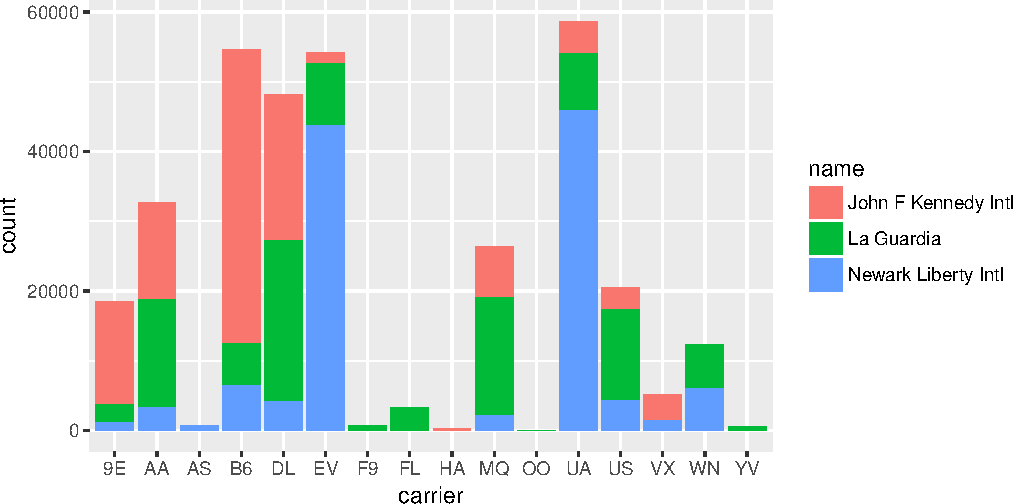
\includegraphics[width=\textwidth]{ismaykim_files/figure-latex/unnamed-chunk-28-1} 

}

\caption[Stacked barplot comparing the number of flights by carrier and airport]{Stacked barplot comparing the number of flights by carrier and airport}\label{fig:unnamed-chunk-28}
\end{figure}

This plot is what is known as a \textbf{stacked barplot}. While simple
to make, it often leads to many problems.

\begin{center}\rule{0.5\linewidth}{\linethickness}\end{center}

\begin{learncheck}
\textbf{\emph{Learning check}}
\end{learncheck}

\textbf{(LC4.32)} What kinds of questions are not easily answered by
looking at the above figure?

\textbf{(LC4.33)} What can you say, if anything, about the relationship
between airline and airport in NYC in 2013 in regards to the number of
departing flights?

\begin{center}\rule{0.5\linewidth}{\linethickness}\end{center}

Another variation on the \textbf{stacked barplot} is the
\textbf{side-by-side barplot}.

\begin{Shaded}
\begin{Highlighting}[]
\KeywordTok{ggplot}\NormalTok{(}\DataTypeTok{data =} \NormalTok{flights_namedports, }\DataTypeTok{mapping =} \KeywordTok{aes}\NormalTok{(}\DataTypeTok{x =} \NormalTok{carrier, }\DataTypeTok{fill =} \NormalTok{name)) +}
\StringTok{  }\KeywordTok{geom_bar}\NormalTok{(}\DataTypeTok{position =} \StringTok{"dodge"}\NormalTok{)}
\end{Highlighting}
\end{Shaded}

\begin{figure}

{\centering 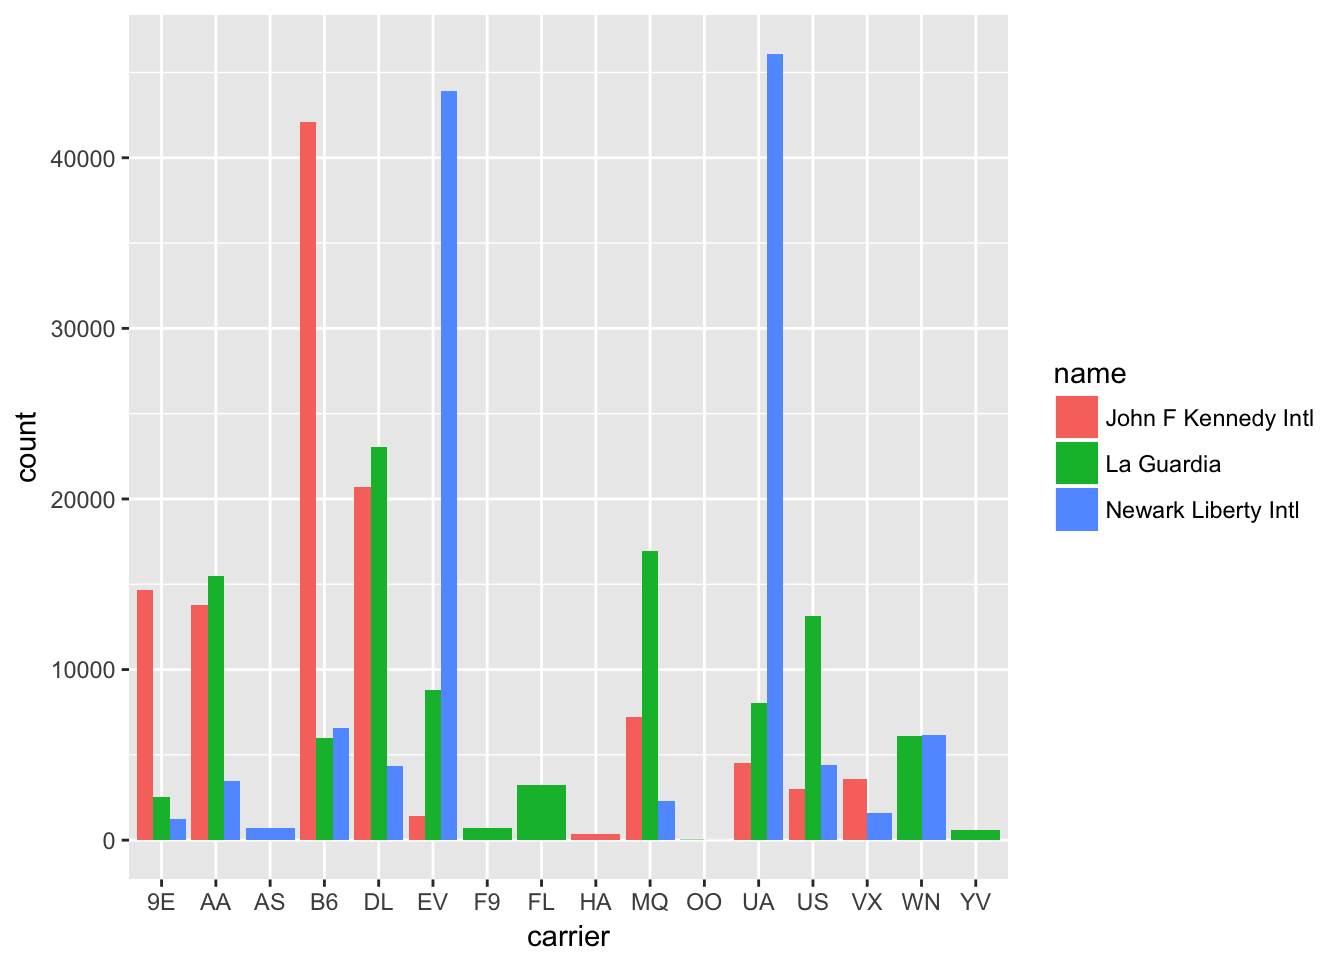
\includegraphics[width=\textwidth]{ismaykim_files/figure-latex/unnamed-chunk-29-1} 

}

\caption[Side-by-side barplot comparing the number of flights by carrier and airport]{Side-by-side barplot comparing the number of flights by carrier and airport}\label{fig:unnamed-chunk-29}
\end{figure}

\begin{center}\rule{0.5\linewidth}{\linethickness}\end{center}

\begin{learncheck}
\textbf{\emph{Learning check}}
\end{learncheck}

\textbf{(LC4.34)} Why might the side-by-side barplot be preferable to a
stacked barplot in this case?

\textbf{(LC4.35)} What are the disadvantages of using a side-by-side
barplot, in general?

\begin{center}\rule{0.5\linewidth}{\linethickness}\end{center}

Lastly, an often preferred type of barplot is the \textbf{faceted
barplot}. We already saw this concept of faceting and small multiples in
Section \ref{facets}. This gives us a nicer way to compare the
distributions across both \texttt{carrier} and airport/\texttt{name}.

\begin{Shaded}
\begin{Highlighting}[]
\KeywordTok{ggplot}\NormalTok{(}\DataTypeTok{data =} \NormalTok{flights_namedports, }\DataTypeTok{mapping =} \KeywordTok{aes}\NormalTok{(}\DataTypeTok{x =} \NormalTok{carrier, }\DataTypeTok{fill =} \NormalTok{name)) +}
\StringTok{  }\KeywordTok{geom_bar}\NormalTok{() +}
\StringTok{  }\KeywordTok{facet_grid}\NormalTok{(name ~}\StringTok{ }\NormalTok{.)}
\end{Highlighting}
\end{Shaded}

\begin{figure}

{\centering 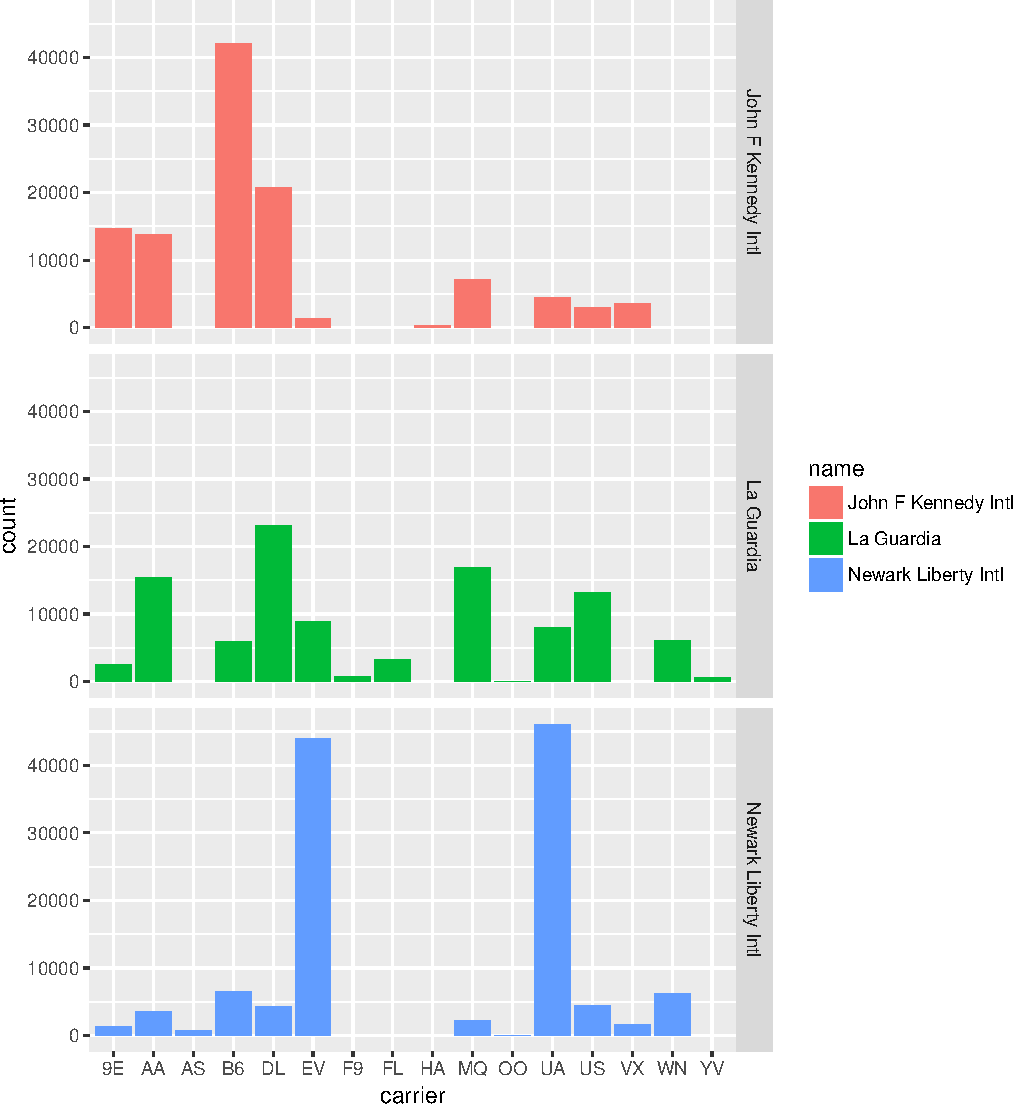
\includegraphics[width=\textwidth]{ismaykim_files/figure-latex/unnamed-chunk-30-1} 

}

\caption[Faceted barplot comparing the number of flights by carrier and airport]{Faceted barplot comparing the number of flights by carrier and airport}\label{fig:unnamed-chunk-30}
\end{figure}

Note how the \texttt{facet\_grid} function arguments are written here.
We are wanting the names of the airports vertically and the
\texttt{carrier} listed horizontally. As you may have guessed, this
argument and other \emph{formulas} of this sort in R are in
\texttt{y\ \textasciitilde{}\ x} order. We will see more examples of
this in Chapter \ref{regress}.

\begin{center}\rule{0.5\linewidth}{\linethickness}\end{center}

\begin{learncheck}
\textbf{\emph{Learning check}}
\end{learncheck}

\textbf{(LC4.36)} Why is the faceted barplot preferred to the
side-by-side and stacked barplots in this case?

\textbf{(LC4.37)} What information about the different carriers at
different airports is more easily seen in the faceted barplot?

\begin{center}\rule{0.5\linewidth}{\linethickness}\end{center}

\subsection{Summary}\label{summary-4}

Barplots are the preferred way of displaying categorical variables. They
are easy-to-understand and to make comparisons across groups of a
categorical variable. When dealing with more than one categorical
variable, faceted barplots are frequently preferred over side-by-side or
stacked barplots. Stacked barplots are sometimes nice to look at, but it
is quite difficult to compare across the levels since the sizes of the
bars are all of different sizes. Side-by-side barplots can provide an
improvement on this, but the issue about comparing across groups still
must be dealt with.

\section{Conclusion}\label{conclusion}

\subsection{Resources}\label{resources}

An excellent resource as you begin to create plots using the
\texttt{ggplot2} package is a cheatsheet that RStudio has put together
entitled ``Data Visualization with ggplot2'' available

\begin{itemize}
\tightlist
\item
  by clicking
  \href{https://www.rstudio.com/wp-content/uploads/2016/11/ggplot2-cheatsheet-2.1.pdf}{here}
  or
\item
  by clicking the RStudio Menu Bar -\textgreater{} Help -\textgreater{}
  Cheatsheets -\textgreater{} ``Data Visualization with
  \texttt{ggplot2}''
\end{itemize}

This covers more than what we've discussed in this chapter but provides
nice visual descriptions of what each function produces.

In addition, we've created a mind map to help you remember which types
of plots are most appropriate in a given situation by identifying the
types of variables involved in the problem. It is available
\href{https://coggle.it/diagram/V_G2gzukTDoQ-aZt-}{here} and below.

\begin{figure}

{\centering 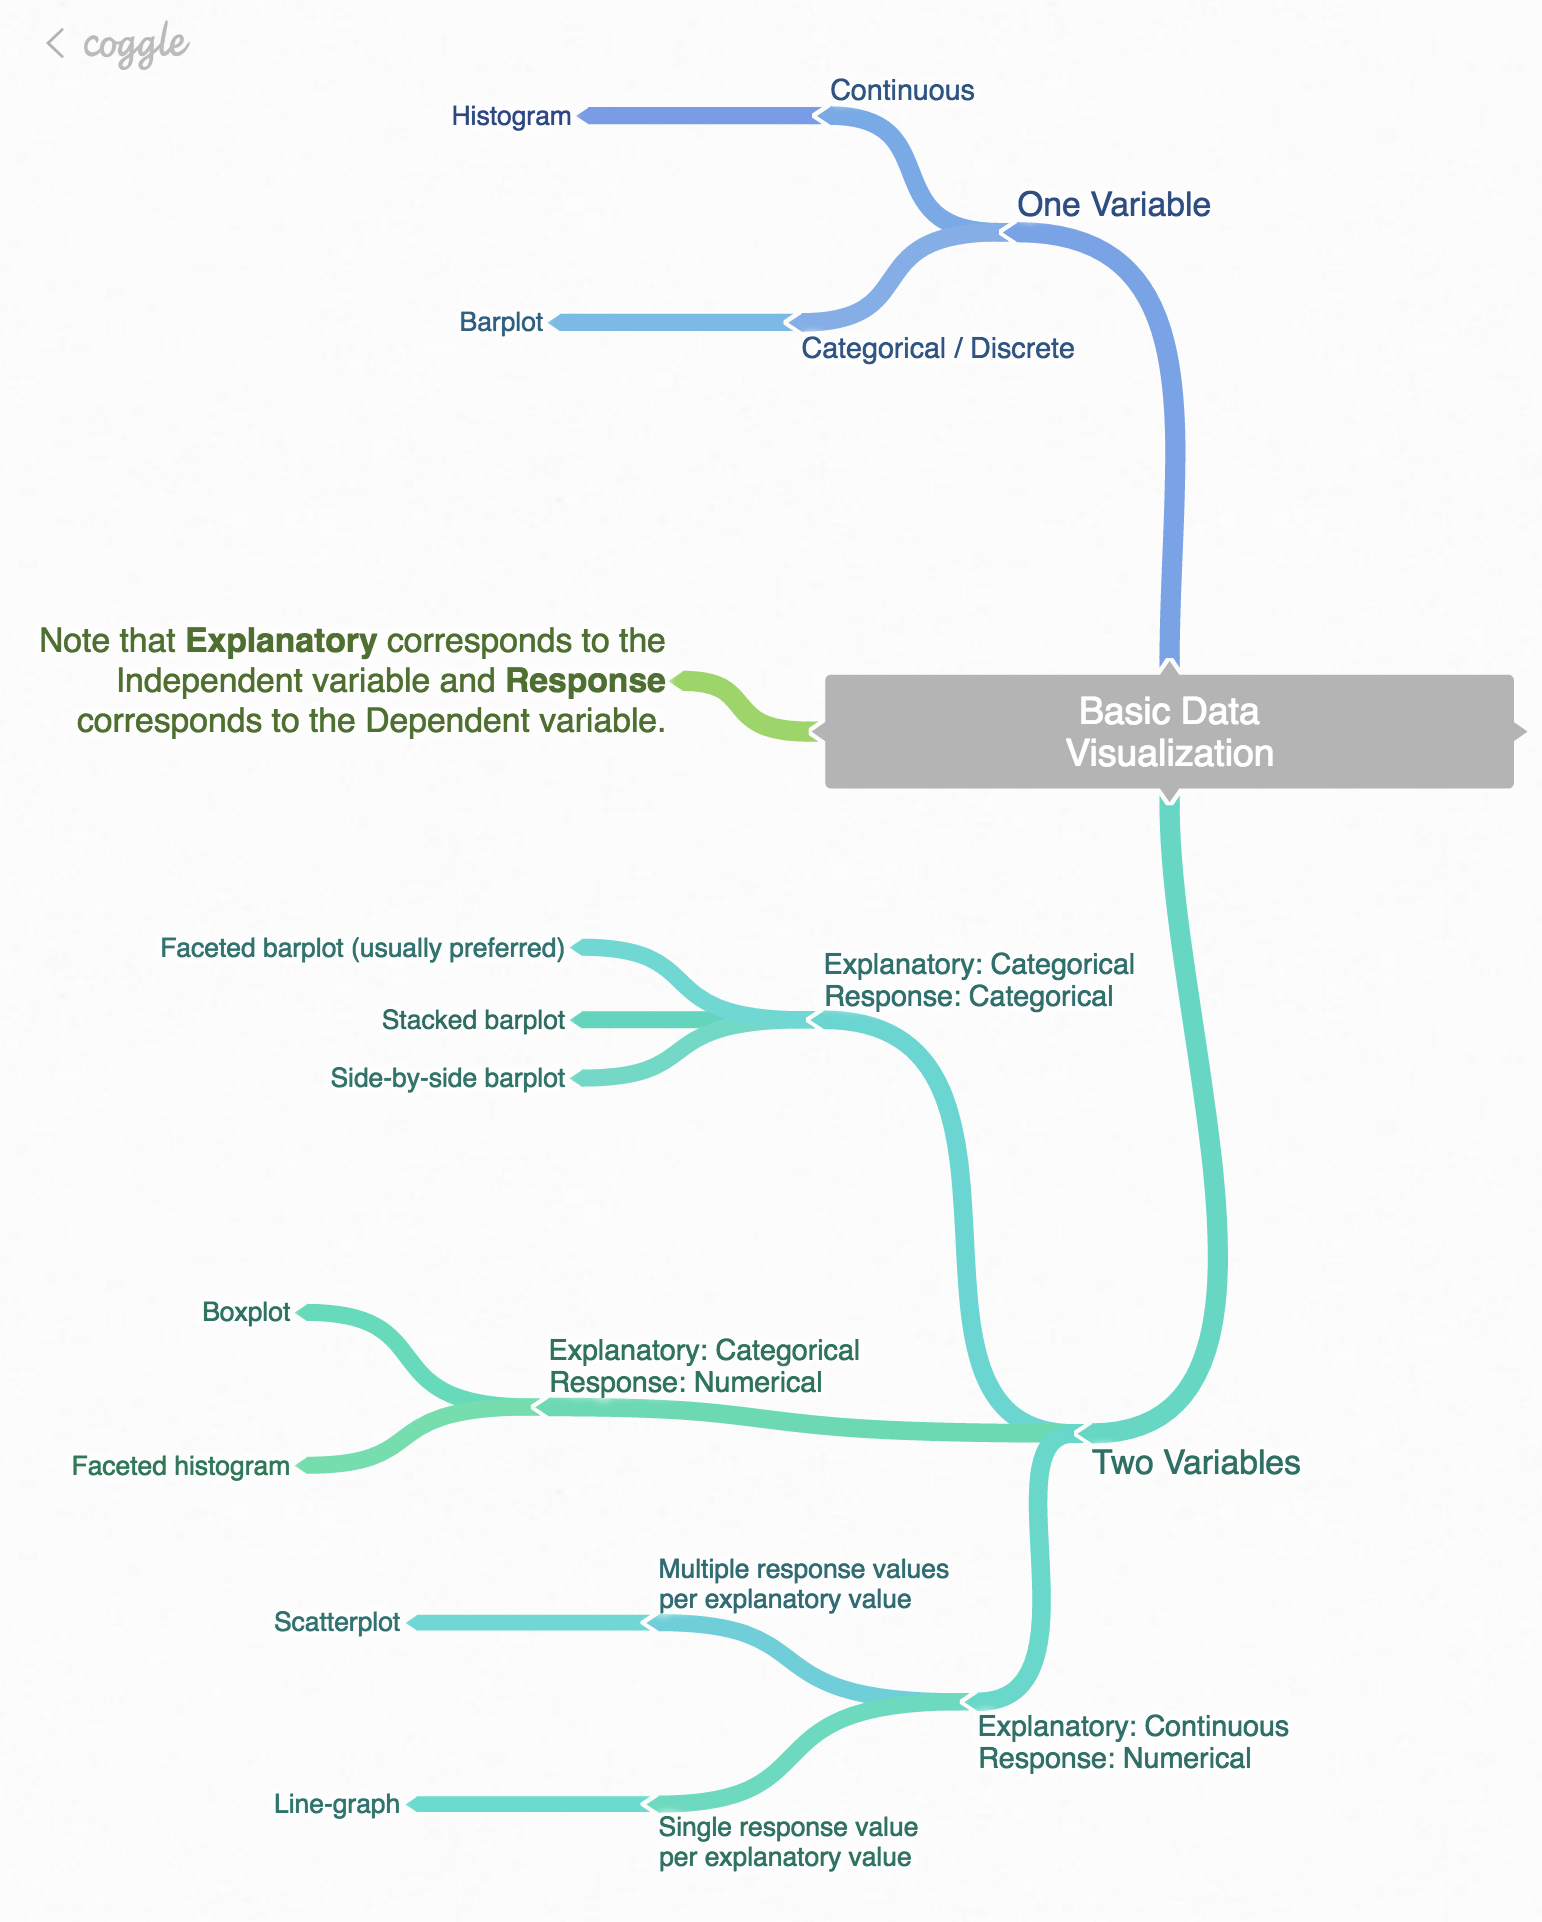
\includegraphics[width=2\linewidth]{images/coggleviz} 

}

\caption[Mind map for Data Visualization]{Mind map for Data Visualization}\label{fig:viz-map}
\end{figure}

\subsection{Script of R code}\label{script-of-r-code}

An R script file of all R code used in this chapter is available
\href{http://ismayc.github.io/moderndiver-book/scripts/04-viz.R}{here}.

\begin{center}\rule{0.5\linewidth}{\linethickness}\end{center}

\begin{center}\rule{0.5\linewidth}{\linethickness}\end{center}

\begin{review}
\textbf{\emph{Review questions}}
\end{review}

Review questions have been designed using the \texttt{fivethirtyeight} R
package \citep{R-fivethirtyeight} with links to the corresponding
FiveThirtyEight.com articles in our free DataCamp course
\textbf{Effective Data Storytelling using the \texttt{tidyverse}}. The
material in this chapter is covered in the chapters of the DataCamp
course available below:

\begin{itemize}
\item
  \href{https://campus.datacamp.com/courses/effective-data-storytelling-using-the-tidyverse/scatter-plots-line-graphs}{Scatter-plots
  \& Line-graphs}
\item
  \href{https://campus.datacamp.com/courses/effective-data-storytelling-using-the-tidyverse/histograms-boxplots}{Histograms
  \& Boxplots}
\item
  \href{https://campus.datacamp.com/courses/effective-data-storytelling-using-the-tidyverse/barplots}{Barplots}
\item
  \href{https://campus.datacamp.com/courses/effective-data-storytelling-using-the-tidyverse/ggplot2-review}{ggplot2
  Review}
\end{itemize}

\begin{center}\rule{0.5\linewidth}{\linethickness}\end{center}

\begin{center}\rule{0.5\linewidth}{\linethickness}\end{center}

\subsection{What's to come?}\label{whats-to-come-1}

In Chapter \ref{manip}, we'll further explore data by grouping our data,
creating summaries based on those groupings, filtering our data to match
conditions, and other manipulations with our data including defining new
columns/variables. These data manipulation procedures will go
hand-in-hand with the data visualizations you've produced here.

\chapter{Data Manipulation via dplyr}\label{manip}

Let's briefly recap where we have been so far and where we are headed.
In Chapter \ref{tidy}, we discussed what it means for data to be tidy.
We saw that this refers to observations corresponding to rows and
variables being stored in columns (one variable for every column). The
entries in the data frame correspond to different combinations of
observations (specific instances of observational units) and variables.
In the \texttt{flights} data frame, we saw that each row corresponds to
a different flight leaving New York City. In other words, the
observational unit of that tidy data frame is a flight. The variables
are listed as columns and for \texttt{flights} they include both
quantitative variables like \texttt{dep\_delay} and \texttt{distance}
but also categorical variables like \texttt{carrier} and
\texttt{origin}. An entry in the table corresponds to a particular
flight on a given day and a particular value of a given variable
representing that flight.

We saw in Chapter \ref{viz} that organizing data in this tidy way makes
it easy for us to produce graphics. We can simply specify what
variable/column we would like on one axis, what variable we'd like on
the other axis, and what type of plot we'd like to make. We can also do
things such as changing the color by another variable or change the size
of our points by a fourth variable given this tidy data set.

Furthermore, in Chapter \ref{viz}, we hinted at some ways to summarize
and manipulate data to suit your needs. This chapter expands on this by
giving a variety of examples using what we call the \emph{Five Main
Verbs} in the \texttt{dplyr} package \citep{R-dplyr}. There are more
advanced operations than just these and you'll see some examples of this
near the end of the chapter.

While at various points we specifically make mention to use the
\texttt{View()} command to inspect a particular data frame, feel free to
do so whenever. In fact, you should get into the habit of doing this for
\emph{any} data frame you work with.

\subsection*{Needed packages}\label{needed-packages-2}
\addcontentsline{toc}{subsection}{Needed packages}

Before we proceed with this chapter, let's load all the necessary
packages.

\begin{Shaded}
\begin{Highlighting}[]
\KeywordTok{library}\NormalTok{(dplyr)}
\KeywordTok{library}\NormalTok{(ggplot2)}
\KeywordTok{library}\NormalTok{(nycflights13)}
\KeywordTok{library}\NormalTok{(knitr)}
\end{Highlighting}
\end{Shaded}

\section{\texorpdfstring{The pipe
\texttt{\%\textgreater{}\%}}{The pipe \%\textgreater{}\%}}\label{the-pipe}

Before we introduce the five main verbs, we first introduce the pipe
operator (\texttt{\%\textgreater{}\%}). Just as the \texttt{+} sign was
used to add layers to a plot created using \texttt{ggplot()}, the pipe
operator allows us to chain together \texttt{dplyr} data manipulation
functions. The pipe operator can be read as ``\emph{then}''. The
\texttt{\%\textgreater{}\%} operator allows us to go from one step in
\texttt{dplyr} to the next easily so we can, for example:

\begin{itemize}
\tightlist
\item
  \texttt{filter} our data frame to only focus on a few rows \emph{then}
\item
  \texttt{group\_by} another variable to create groups \emph{then}
\item
  \texttt{summarize} this grouped data to calculate the mean for each
  level of the group.
\end{itemize}

The piping syntax will be our major focus throughout the rest of this
book and you'll find that you'll quickly be addicted to the chaining
with some practice. If you'd like to see more examples on using
\texttt{dplyr}, the 5MV (in addition to some other \texttt{dplyr}
verbs), and \texttt{\%\textgreater{}\%} with the \texttt{nycflights13}
data set, you can check out Chapter 5 of Hadley and Garrett's book
\citep{rds2016}.

\section{Five Main Verbs - The 5MV}\label{five-main-verbs---the-5mv}

The \texttt{d} in \texttt{dplyr} stands for data frames, so the
functions here work when you are working with objects of the data frame
type. It's most important for you to focus on the 5MV: the five most
commonly used functions that help us manipulate and summarize data. A
description of these verbs follows with each subsection devoted to
seeing an example of that verb in play (or a combination of a few
verbs):

\begin{itemize}
\tightlist
\item
  \texttt{filter}: Pick rows based on conditions about their values
\item
  \texttt{summarize}: Create summary measures of variables either

  \begin{itemize}
  \tightlist
  \item
    over the entire data frame
  \item
    or over groups of observations on variables using \texttt{group\_by}
  \end{itemize}
\item
  \texttt{mutate}: Create a new variable in the data frame by mutating
  existing ones
\item
  \texttt{arrange}: Arrange/sort the rows based on one or more variables
\end{itemize}

Just as we had the 5NG (The Five Named Graphs in Chapter \ref{viz} using
\texttt{ggplot2}) for data visualization, we also have the 5MV here (The
Five Main Verbs in \texttt{dplyr}) for data manipulation. All of the
5MVs follow the same syntax with the argument before the pipe
\texttt{\%\textgreater{}\%} being the name of the data frame and then
the name of the verb with other arguments specifying which criteria
you'd like the verb to work with in parentheses.

\subsection{5MV\#1: Filter observations using filter}\label{filter}

\begin{figure}

{\centering 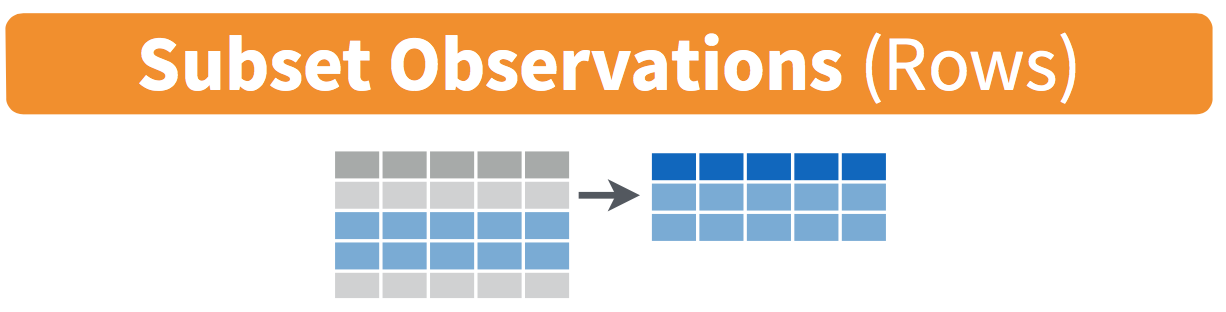
\includegraphics[width=\textwidth]{images/filter} 

}

\caption[Filter diagram from Data Wrangling with dplyr and tidyr cheatsheet]{Filter diagram from Data Wrangling with dplyr and tidyr cheatsheet}\label{fig:filter}
\end{figure}

The \texttt{filter} function here works much like the ``Filter'' option
in Microsoft Excel; it allows you to specify criteria about values of a
variable in your data set and then chooses only those rows that match
that criteria. We begin by focusing only on flights from New York City
to Portland, Oregon. The \texttt{dest} code (or airport code) for
Portland, Oregon is \texttt{"PDX"}. Run the following and look at the
resulting spreadsheet to ensure that only flights heading to Portland
are chosen here:

\begin{Shaded}
\begin{Highlighting}[]
\NormalTok{portland_flights <-}\StringTok{ }\NormalTok{flights %>%}\StringTok{ }
\StringTok{  }\KeywordTok{filter}\NormalTok{(dest ==}\StringTok{ "PDX"}\NormalTok{)}
\KeywordTok{View}\NormalTok{(portland_flights)}
\end{Highlighting}
\end{Shaded}

Note the following:

\begin{itemize}
\tightlist
\item
  The ordering of the commands:

  \begin{itemize}
  \tightlist
  \item
    Take the data frame \texttt{flights} \emph{then}
  \item
    \texttt{filter} the data frame so that only those where the
    \texttt{dest} equals \texttt{"PDX"} are included.
  \end{itemize}
\item
  The double equal sign \texttt{==} You are almost guaranteed to make
  the mistake at least once of only including one equals sign. Let's see
  what happens when we make this error:
\end{itemize}

\begin{Shaded}
\begin{Highlighting}[]
\NormalTok{portland_flights <-}\StringTok{ }\NormalTok{flights %>%}\StringTok{ }
\StringTok{  }\KeywordTok{filter}\NormalTok{(}\DataTypeTok{dest =} \StringTok{"PDX"}\NormalTok{)}
\end{Highlighting}
\end{Shaded}

\begin{verbatim}
Error: filter() takes unnamed arguments. Do you need `==`?
\end{verbatim}

You can combine multiple criteria together using operators that make
comparisons:

\begin{itemize}
\tightlist
\item
  \texttt{\textbar{}} corresponds to ``or''
\item
  \texttt{\&} corresponds to ``and''
\end{itemize}

We can often skip the use of \texttt{\&} and just separate our
conditions with a comma. You'll see this in the example below.

In addition, you can use other mathematical checks (similar to
\texttt{==}):

\begin{itemize}
\tightlist
\item
  \texttt{\textgreater{}} corresponds to ``greater than''
\item
  \texttt{\textless{}} corresponds to ``less than''
\item
  \texttt{\textgreater{}=} corresponds to ``greater than or equal to''
\item
  \texttt{\textless{}=} corresponds to ``less than or equal to''
\item
  \texttt{!=} corresponds to ``not equal to''
\end{itemize}

To see many of these in action, let's select all flights that left JFK
airport heading to Burlington, Vermont (\texttt{"BTV"}) or Seattle,
Washington (\texttt{"SEA"}) in the months of October, November, or
December. Run the following

\begin{Shaded}
\begin{Highlighting}[]
\NormalTok{btv_sea_flights_fall <-}\StringTok{ }\NormalTok{flights %>%}\StringTok{ }
\StringTok{  }\KeywordTok{filter}\NormalTok{(origin ==}\StringTok{ "JFK"}\NormalTok{, (dest ==}\StringTok{ "BTV"} \NormalTok{|}\StringTok{ }\NormalTok{dest ==}\StringTok{ "SEA"}\NormalTok{), month >=}\StringTok{ }\DecValTok{10}\NormalTok{)}
\KeywordTok{View}\NormalTok{(btv_sea_flights_fall)}
\end{Highlighting}
\end{Shaded}

Note how even though colloquially speaking one might say ``all flights
leaving Burlington, Vermont \emph{and} Seattle, Washington'', in terms
of computer operations, we really mean ``all flights leaving Burlington,
Vermont \emph{or} Seattle, Washington'', because for a given row in the
data, \texttt{dest} can either be: ``BTV'', ``SEA'', or something else,
but not ``BTV'' and ``SEA'' at the same time.

Another example uses the \texttt{!} to pick rows that \textbf{DON'T}
match a condition. Here we are selecting rows corresponding to flights
that didn't go to Burlington, VT or Seattle, WA.

\begin{Shaded}
\begin{Highlighting}[]
\NormalTok{not_BTV_SEA <-}\StringTok{ }\NormalTok{flights %>%}\StringTok{ }
\StringTok{  }\KeywordTok{filter}\NormalTok{(!(dest ==}\StringTok{ "BTV"} \NormalTok{|}\StringTok{ }\NormalTok{dest ==}\StringTok{ "SEA"}\NormalTok{))}
\KeywordTok{View}\NormalTok{(not_BTV_SEA)}
\end{Highlighting}
\end{Shaded}

As a final note we point out that \texttt{filter()} should often be the
first verb you'll apply to your data. This cleans your data set to only
those rows you care about, or put differently, it narrows down the scope
to just the observations your care about.

\begin{center}\rule{0.5\linewidth}{\linethickness}\end{center}

\begin{learncheck}
\textbf{\emph{Learning check}}
\end{learncheck}

\textbf{(LC5.1)} What's another way using \texttt{!} we could filter
only the rows that are not going to Burlington, VT nor Seattle, WA in
the \texttt{flights} data frame? Test this out using the code above.

\begin{center}\rule{0.5\linewidth}{\linethickness}\end{center}

\subsection{5MV\#2: Summarize variables using
summarize}\label{mv2-summarize-variables-using-summarize}

\begin{figure}

{\centering 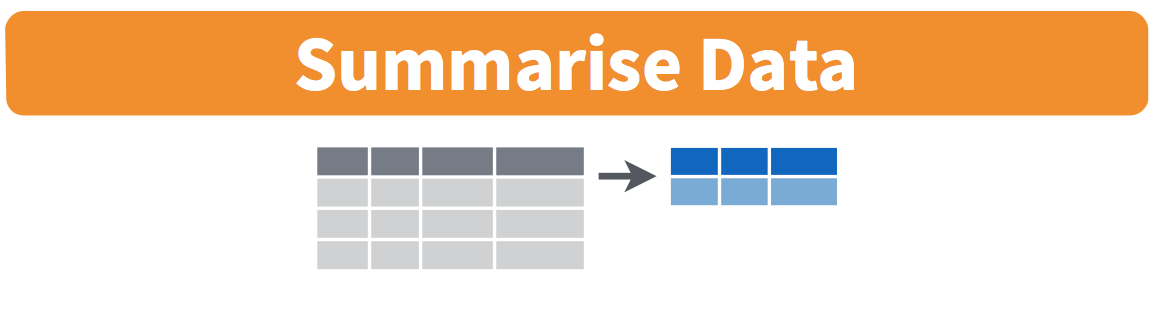
\includegraphics[width=\textwidth]{images/summarize1} 

}

\caption[Summarize diagram from Data Wrangling with dplyr and tidyr cheatsheet]{Summarize diagram from Data Wrangling with dplyr and tidyr cheatsheet}\label{fig:sum1}
\end{figure}

\begin{figure}

{\centering 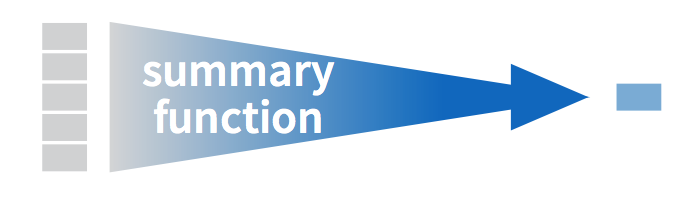
\includegraphics[width=\textwidth]{images/summary} 

}

\caption[Another summarize diagram from Data Wrangling with dplyr and tidyr cheatsheet]{Another summarize diagram from Data Wrangling with dplyr and tidyr cheatsheet}\label{fig:sum2}
\end{figure}

We can calculate the standard deviation and mean of the temperature
variable \texttt{temp} in the \texttt{weather} data frame of
\texttt{nycflights13} in one step using the \texttt{summarize} function
in \texttt{dplyr}:

\begin{Shaded}
\begin{Highlighting}[]
\NormalTok{summary_temp <-}\StringTok{ }\NormalTok{weather %>%}\StringTok{ }
\StringTok{  }\KeywordTok{summarize}\NormalTok{(}\DataTypeTok{mean =} \KeywordTok{mean}\NormalTok{(temp), }\DataTypeTok{std_dev =} \KeywordTok{sd}\NormalTok{(temp))}
\KeywordTok{kable}\NormalTok{(summary_temp)}
\end{Highlighting}
\end{Shaded}

\begin{tabular}{r|r}
\hline
mean & std\_dev\\
\hline
NA & NA\\
\hline
\end{tabular}

We've created a small data frame here called \texttt{summary\_temp} that
includes both the \texttt{mean} and the \texttt{std\_dev} of the
\texttt{temp} variable in \texttt{weather}. Notice as shown in Figures
\ref{fig:sum1} and \ref{fig:sum2}, the data frame \texttt{weather} went
from many rows to a single row of just the summary values in the data
frame \texttt{summary\_temp}. But why are the mean and standard
deviation missing, i.e. \texttt{NA}? Remember that by default the
\texttt{mean} and \texttt{sd} functions do not ignore missing values. We
need to specify the argument \texttt{na.rm=TRUE} (\texttt{rm} is short
for ``remove''):

\begin{Shaded}
\begin{Highlighting}[]
\NormalTok{summary_temp <-}\StringTok{ }\NormalTok{weather %>%}\StringTok{ }
\StringTok{  }\KeywordTok{summarize}\NormalTok{(}\DataTypeTok{mean =} \KeywordTok{mean}\NormalTok{(temp, }\DataTypeTok{na.rm =} \OtherTok{TRUE}\NormalTok{), }\DataTypeTok{std_dev =} \KeywordTok{sd}\NormalTok{(temp, }\DataTypeTok{na.rm =} \OtherTok{TRUE}\NormalTok{))}
\KeywordTok{kable}\NormalTok{(summary_temp)}
\end{Highlighting}
\end{Shaded}

\begin{tabular}{r|r}
\hline
mean & std\_dev\\
\hline
55.2 & 17.78\\
\hline
\end{tabular}

If we'd like to access either of these values directly we can use the
\texttt{\$} to specify a column in a data frame. For example:

\begin{Shaded}
\begin{Highlighting}[]
\NormalTok{summary_temp$mean}
\end{Highlighting}
\end{Shaded}

\begin{verbatim}
## [1] 55.2
\end{verbatim}

You'll often encounter issues with missing values \texttt{NA}. In fact,
an entire branch of the field of statistics deals with missing data.
However, it is not good practice to include a \texttt{na.rm\ =\ TRUE} in
your summary commands by default; you should attempt to run them without
this argument. The idea being you should at the very least be alerted to
the presence of missing values and consider what the impact on the
analysis might be if you ignore these values. In other words,
\texttt{na.rm\ =\ TRUE} should only be used when necessary.

What other summary functions can we use inside the \texttt{summarize()}
verb? Any function in R that takes a vector of values and returns just
one. Here are just a few:

\begin{itemize}
\tightlist
\item
  \texttt{min()} and \texttt{max()}: the minimum and maximum values
  respectively
\item
  \texttt{IQR()}: Interquartile range
\item
  \texttt{sum()}: the sum
\item
  \texttt{n()}: a count of the number of rows/observations in each
  group. This particular summary function will make more sense in the
  \texttt{group\_by} chapter.
\end{itemize}

\begin{center}\rule{0.5\linewidth}{\linethickness}\end{center}

\begin{learncheck}
\textbf{\emph{Learning check}}
\end{learncheck}

\textbf{(LC5.2)} Say a doctor is studying the effect of smoking on lung
cancer of a large number of patients who have records measured at five
year intervals. He notices that a large number of patients have missing
data points because the patient has died, so he chooses to ignore these
patients in his analysis. What is wrong with this doctor's approach?

\textbf{(LC5.3)} Modify the above \texttt{summarize} function to create
\texttt{summary\_temp} to also use the \texttt{n()} summary function:
\texttt{summarize(count\ =\ n())}. What does the returned value
correspond to?

\textbf{(LC5.4)} Why doesn't the following code work? You may want to
run the code line by line instead of all at once. In other words, run
\texttt{summary\_temp\ \textless{}-\ weather\ \%\textgreater{}\%\ summarize(mean\ =\ mean(temp,\ na.rm\ =\ TRUE))}
first.

\begin{Shaded}
\begin{Highlighting}[]
\NormalTok{summary_temp <-}\StringTok{ }\NormalTok{weather %>%}\StringTok{   }
\StringTok{  }\KeywordTok{summarize}\NormalTok{(}\DataTypeTok{mean =} \KeywordTok{mean}\NormalTok{(temp, }\DataTypeTok{na.rm =} \OtherTok{TRUE}\NormalTok{)) %>%}\StringTok{ }
\StringTok{  }\KeywordTok{summarize}\NormalTok{(}\DataTypeTok{std_dev =} \KeywordTok{sd}\NormalTok{(temp, }\DataTypeTok{na.rm =} \OtherTok{TRUE}\NormalTok{))}
\end{Highlighting}
\end{Shaded}

\begin{center}\rule{0.5\linewidth}{\linethickness}\end{center}

\subsection{5MV\#3: Group rows using
group\_by}\label{mv3-group-rows-using-group_by}

\begin{figure}

{\centering 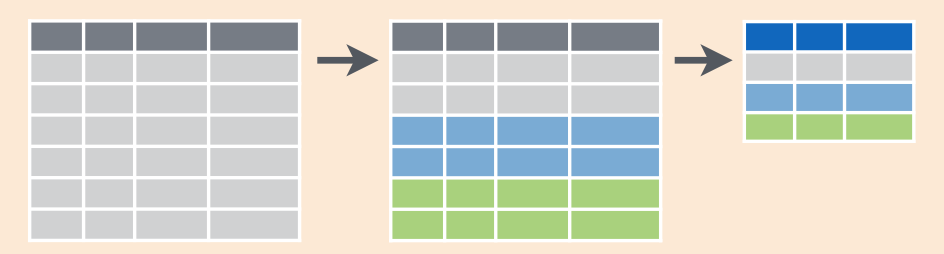
\includegraphics[width=\textwidth]{images/group_summary} 

}

\caption[Group by and summarize diagram from Data Wrangling with dplyr and tidyr cheatsheet]{Group by and summarize diagram from Data Wrangling with dplyr and tidyr cheatsheet}\label{fig:groupsummarize}
\end{figure}

However, it's often more useful to summarize a variable based on the
groupings of another variable. Let's say similarly to the previous
section, we are interested in the mean and standard deviation of
temperatures but \emph{grouped by month}. This concept can equivalently
be articulated as: we want the mean and standard deviation of
temperatures

\begin{enumerate}
\def\labelenumi{\arabic{enumi}.}
\tightlist
\item
  split by month.
\item
  sliced by month.
\item
  aggregated by month.
\item
  collapsed over month.
\end{enumerate}

We believe that you will be amazed at just how simple this is. Run the
following code:

\begin{Shaded}
\begin{Highlighting}[]
\NormalTok{summary_monthly_temp <-}\StringTok{ }\NormalTok{weather %>%}\StringTok{ }
\StringTok{  }\KeywordTok{group_by}\NormalTok{(month) %>%}\StringTok{ }
\StringTok{  }\KeywordTok{summarize}\NormalTok{(}\DataTypeTok{mean =} \KeywordTok{mean}\NormalTok{(temp, }\DataTypeTok{na.rm =} \OtherTok{TRUE}\NormalTok{), }
            \DataTypeTok{std_dev =} \KeywordTok{sd}\NormalTok{(temp, }\DataTypeTok{na.rm =} \OtherTok{TRUE}\NormalTok{))}
\KeywordTok{kable}\NormalTok{(summary_monthly_temp)}
\end{Highlighting}
\end{Shaded}

\begin{tabular}{r|r|r}
\hline
month & mean & std\_dev\\
\hline
1 & 35.64 & 10.185\\
\hline
2 & 34.15 & 6.940\\
\hline
3 & 39.81 & 6.225\\
\hline
4 & 51.67 & 8.785\\
\hline
5 & 61.59 & 9.609\\
\hline
6 & 72.14 & 7.603\\
\hline
7 & 80.01 & 7.148\\
\hline
8 & 74.40 & 5.171\\
\hline
9 & 67.43 & 8.476\\
\hline
10 & 60.03 & 8.830\\
\hline
11 & 45.11 & 10.502\\
\hline
12 & 38.37 & 9.941\\
\hline
\end{tabular}

This code is identical to the previous code that created
\texttt{summary\_temp}, but there is an extra \texttt{group\_by(month)}
spliced in between. By simply grouping the \texttt{weather} data set by
\texttt{month} first and then passing this new data frame into
\texttt{summarize} we get a resulting data frame that shows the mean and
standard deviation temperature for each month in New York City. Since
each row in \texttt{summary\_monthly\_temp} represents a summary of
different rows in \texttt{weather}, the observational units have
changed.

It is important to note that \texttt{group\_by} doesn't actually change
the data frame. It simply sets \emph{meta-data} (data about the data),
specifically the group structure of the data. It is only after we apply
the \texttt{summarize} function that the data frame actually changes. If
we would like to remove this group structure meta-data, we can pipe a
resulting data frame into the \texttt{ungroup()} function.

We now revisit the \texttt{n()} counting summary function we introduced
in the previous section. For example, suppose we'd like to get a sense
for how many flights departed each of the three airports in New York
City:

\begin{Shaded}
\begin{Highlighting}[]
\NormalTok{by_origin <-}\StringTok{ }\NormalTok{flights %>%}\StringTok{ }
\StringTok{  }\KeywordTok{group_by}\NormalTok{(origin) %>%}\StringTok{ }
\StringTok{  }\KeywordTok{summarize}\NormalTok{(}\DataTypeTok{count =} \KeywordTok{n}\NormalTok{())}
\KeywordTok{kable}\NormalTok{(by_origin)}
\end{Highlighting}
\end{Shaded}

\begin{tabular}{l|r}
\hline
origin & count\\
\hline
EWR & 120835\\
\hline
JFK & 111279\\
\hline
LGA & 104662\\
\hline
\end{tabular}

We see that Newark (\texttt{"EWR"}) had the most flights departing in
2013 followed by \texttt{"JFK"} and lastly by LaGuardia
(\texttt{"LGA"}). Note there is a subtle but important difference
between \texttt{sum()} and \texttt{n()}. While \texttt{sum()} simply
adds up a large set of numbers, the latter counts the number of times
each of many different values occur.

You are not limited to grouping by one variable! Say you wanted to know
the number of flights leaving each of the three New York City airports
\emph{for each month}, we can also group by a second variable
\texttt{month}: \texttt{group\_by(origin,\ month)}.

\begin{Shaded}
\begin{Highlighting}[]
\NormalTok{by_monthly_origin <-}\StringTok{ }\NormalTok{flights %>%}\StringTok{ }
\StringTok{  }\KeywordTok{group_by}\NormalTok{(origin, month) %>%}\StringTok{ }
\StringTok{  }\KeywordTok{summarize}\NormalTok{(}\DataTypeTok{count =} \KeywordTok{n}\NormalTok{())}
\KeywordTok{kable}\NormalTok{(by_monthly_origin)}
\end{Highlighting}
\end{Shaded}

\begin{tabular}{l|r|r}
\hline
origin & month & count\\
\hline
EWR & 1 & 9893\\
\hline
EWR & 2 & 9107\\
\hline
EWR & 3 & 10420\\
\hline
EWR & 4 & 10531\\
\hline
EWR & 5 & 10592\\
\hline
EWR & 6 & 10175\\
\hline
EWR & 7 & 10475\\
\hline
EWR & 8 & 10359\\
\hline
EWR & 9 & 9550\\
\hline
EWR & 10 & 10104\\
\hline
EWR & 11 & 9707\\
\hline
EWR & 12 & 9922\\
\hline
JFK & 1 & 9161\\
\hline
JFK & 2 & 8421\\
\hline
JFK & 3 & 9697\\
\hline
JFK & 4 & 9218\\
\hline
JFK & 5 & 9397\\
\hline
JFK & 6 & 9472\\
\hline
JFK & 7 & 10023\\
\hline
JFK & 8 & 9983\\
\hline
JFK & 9 & 8908\\
\hline
JFK & 10 & 9143\\
\hline
JFK & 11 & 8710\\
\hline
JFK & 12 & 9146\\
\hline
LGA & 1 & 7950\\
\hline
LGA & 2 & 7423\\
\hline
LGA & 3 & 8717\\
\hline
LGA & 4 & 8581\\
\hline
LGA & 5 & 8807\\
\hline
LGA & 6 & 8596\\
\hline
LGA & 7 & 8927\\
\hline
LGA & 8 & 8985\\
\hline
LGA & 9 & 9116\\
\hline
LGA & 10 & 9642\\
\hline
LGA & 11 & 8851\\
\hline
LGA & 12 & 9067\\
\hline
\end{tabular}

Alternatively, you can use the shortcut \texttt{count()} function in
\texttt{dplyr} to get the same result:

\begin{Shaded}
\begin{Highlighting}[]
\NormalTok{by_monthly_origin2 <-}\StringTok{ }\NormalTok{flights %>%}\StringTok{ }
\StringTok{  }\NormalTok{dplyr::}\KeywordTok{count}\NormalTok{(origin, month)}
\KeywordTok{kable}\NormalTok{(by_monthly_origin2)}
\end{Highlighting}
\end{Shaded}

\begin{tabular}{l|r|r}
\hline
origin & month & n\\
\hline
EWR & 1 & 9893\\
\hline
EWR & 2 & 9107\\
\hline
EWR & 3 & 10420\\
\hline
EWR & 4 & 10531\\
\hline
EWR & 5 & 10592\\
\hline
EWR & 6 & 10175\\
\hline
EWR & 7 & 10475\\
\hline
EWR & 8 & 10359\\
\hline
EWR & 9 & 9550\\
\hline
EWR & 10 & 10104\\
\hline
EWR & 11 & 9707\\
\hline
EWR & 12 & 9922\\
\hline
JFK & 1 & 9161\\
\hline
JFK & 2 & 8421\\
\hline
JFK & 3 & 9697\\
\hline
JFK & 4 & 9218\\
\hline
JFK & 5 & 9397\\
\hline
JFK & 6 & 9472\\
\hline
JFK & 7 & 10023\\
\hline
JFK & 8 & 9983\\
\hline
JFK & 9 & 8908\\
\hline
JFK & 10 & 9143\\
\hline
JFK & 11 & 8710\\
\hline
JFK & 12 & 9146\\
\hline
LGA & 1 & 7950\\
\hline
LGA & 2 & 7423\\
\hline
LGA & 3 & 8717\\
\hline
LGA & 4 & 8581\\
\hline
LGA & 5 & 8807\\
\hline
LGA & 6 & 8596\\
\hline
LGA & 7 & 8927\\
\hline
LGA & 8 & 8985\\
\hline
LGA & 9 & 9116\\
\hline
LGA & 10 & 9642\\
\hline
LGA & 11 & 8851\\
\hline
LGA & 12 & 9067\\
\hline
\end{tabular}

\begin{center}\rule{0.5\linewidth}{\linethickness}\end{center}

\begin{learncheck}
\textbf{\emph{Learning check}}
\end{learncheck}

\textbf{(LC5.5)} Recall from Chapter \ref{viz} when we looked at plots
of temperatures by months in NYC. What does the standard deviation
column in the \texttt{summary\_monthly\_temp} data frame tell us about
temperatures in New York City throughout the year?

\textbf{(LC5.6)} What code would be required to get the mean and
standard deviation temperature for each day in 2013 for NYC?

\textbf{(LC5.7)} Recreate \texttt{by\_monthly\_origin}, but instead of
grouping via \texttt{group\_by(origin,\ month)}, group variables in a
different order \texttt{group\_by(month,\ origin)}. What differs in the
resulting data set?

\textbf{(LC5.8)} How could we identify how many flights left each of the
three airports for each \texttt{carrier}?

\textbf{(LC5.9)} How does the \texttt{filter} operation differ from a
\texttt{group\_by} followed by a \texttt{summarize}?

\begin{center}\rule{0.5\linewidth}{\linethickness}\end{center}

\subsection{5MV\#4: Create new variables/change old variables using
mutate}\label{mv4-create-new-variableschange-old-variables-using-mutate}

\begin{figure}

{\centering 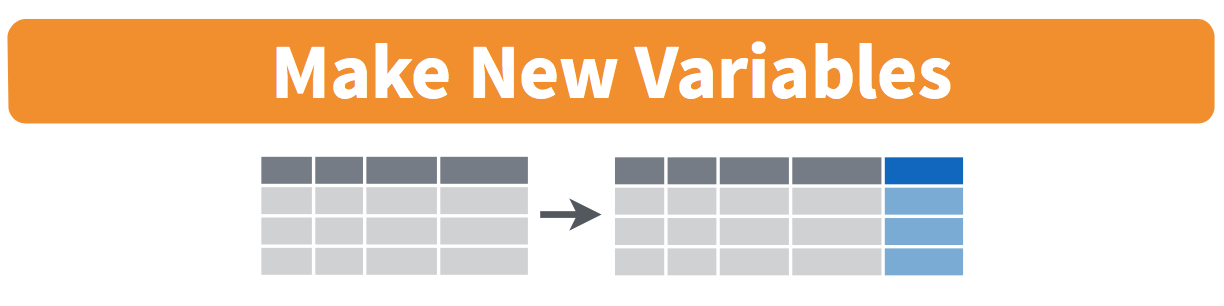
\includegraphics[width=\textwidth]{images/mutate} 

}

\caption[Mutate diagram from Data Wrangling with dplyr and tidyr cheatsheet]{Mutate diagram from Data Wrangling with dplyr and tidyr cheatsheet}\label{fig:select}
\end{figure}

When looking at the \texttt{flights} data set, there are some clear
additional variables that could be calculated based on the values of
variables already in the data set. Passengers are often frustrated when
their flights departs late, but change their mood a bit if pilots can
make up some time during the flight to get them to their destination
close to when they expected to land. This is commonly referred to as
``gain'' and we will create this variable using the \texttt{mutate}
function. Note that we have also overwritten the \texttt{flights} data
frame with what it was before as well as an additional variable
\texttt{gain} here.

\begin{Shaded}
\begin{Highlighting}[]
\NormalTok{flights <-}\StringTok{ }\NormalTok{flights %>%}\StringTok{ }
\StringTok{  }\KeywordTok{mutate}\NormalTok{(}\DataTypeTok{gain =} \NormalTok{arr_delay -}\StringTok{ }\NormalTok{dep_delay)}
\end{Highlighting}
\end{Shaded}

Why did we overwrite \texttt{flights} instead of assigning the resulting
data frame to a new object, like \texttt{flights\_with\_gain}? As a
rough rule of thumb, as long as you are not losing information that you
might need later, its acceptable practice to overwrite data frames.
However, if you overwrite existing variables and/or change the
observational units, recovering the original information might prove
difficult. In this case, it might make sense to create a new data
object.

Let's look at summary measures of this \texttt{gain} variable and even
plot it in the form of a histogram:

\begin{Shaded}
\begin{Highlighting}[]
\NormalTok{gain_summary <-}\StringTok{ }\NormalTok{flights %>%}\StringTok{ }
\StringTok{  }\KeywordTok{summarize}\NormalTok{(}
    \DataTypeTok{min =} \KeywordTok{min}\NormalTok{(gain, }\DataTypeTok{na.rm =} \OtherTok{TRUE}\NormalTok{),}
    \DataTypeTok{q1 =} \KeywordTok{quantile}\NormalTok{(gain, }\FloatTok{0.25}\NormalTok{, }\DataTypeTok{na.rm =} \OtherTok{TRUE}\NormalTok{),}
    \DataTypeTok{median =} \KeywordTok{quantile}\NormalTok{(gain, }\FloatTok{0.5}\NormalTok{, }\DataTypeTok{na.rm =} \OtherTok{TRUE}\NormalTok{),}
    \DataTypeTok{q3 =} \KeywordTok{quantile}\NormalTok{(gain, }\FloatTok{0.75}\NormalTok{, }\DataTypeTok{na.rm =} \OtherTok{TRUE}\NormalTok{),}
    \DataTypeTok{max =} \KeywordTok{max}\NormalTok{(gain, }\DataTypeTok{na.rm =} \OtherTok{TRUE}\NormalTok{),}
    \DataTypeTok{mean =} \KeywordTok{mean}\NormalTok{(gain, }\DataTypeTok{na.rm =} \OtherTok{TRUE}\NormalTok{),}
    \DataTypeTok{sd =} \KeywordTok{sd}\NormalTok{(gain, }\DataTypeTok{na.rm =} \OtherTok{TRUE}\NormalTok{),}
    \DataTypeTok{missing =} \KeywordTok{sum}\NormalTok{(}\KeywordTok{is.na}\NormalTok{(gain))}
  \NormalTok{)}
\KeywordTok{kable}\NormalTok{(gain_summary)}
\end{Highlighting}
\end{Shaded}

\begin{tabular}{r|r|r|r|r|r|r|r}
\hline
min & q1 & median & q3 & max & mean & sd & missing\\
\hline
-109 & -17 & -7 & 3 & 196 & -5.66 & 18.04 & 9430\\
\hline
\end{tabular}

We've recreated the \texttt{summary} function we saw in Chapter
\ref{viz} here using the \texttt{summarize} function in \texttt{dplyr}.

\begin{Shaded}
\begin{Highlighting}[]
\KeywordTok{ggplot}\NormalTok{(}\DataTypeTok{data =} \NormalTok{flights, }\DataTypeTok{mapping =} \KeywordTok{aes}\NormalTok{(}\DataTypeTok{x =} \NormalTok{gain)) +}
\StringTok{  }\KeywordTok{geom_histogram}\NormalTok{(}\DataTypeTok{color =} \StringTok{"white"}\NormalTok{, }\DataTypeTok{bins =} \DecValTok{20}\NormalTok{)}
\end{Highlighting}
\end{Shaded}

\begin{figure}

{\centering 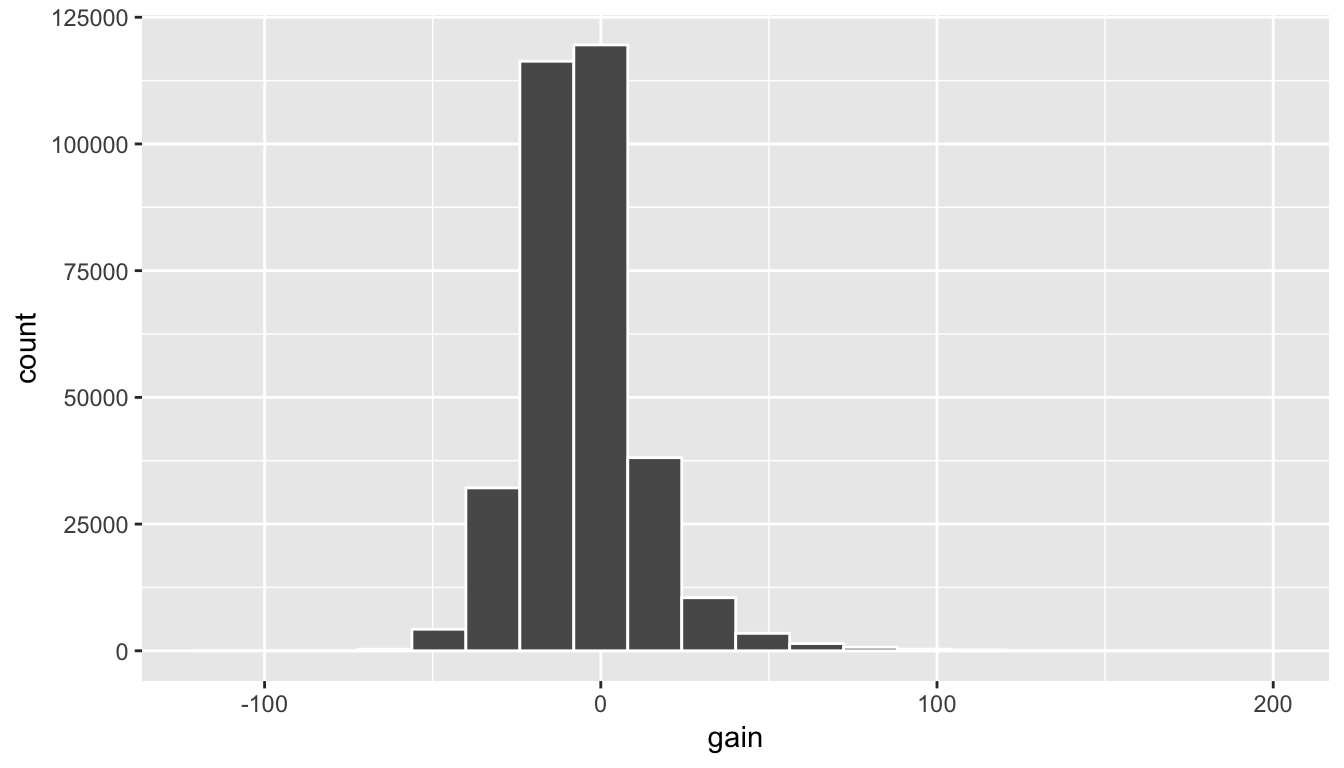
\includegraphics[width=\textwidth]{ismaykim_files/figure-latex/unnamed-chunk-48-1} 

}

\caption[Histogram of gain variable]{Histogram of gain variable}\label{fig:unnamed-chunk-48}
\end{figure}

We can also create multiple columns at once and even refer to columns
that were just created in a new column. Hadley produces one such example
in Chapter 5 of ``R for Data Science'' \citep{rds2016}:

\begin{Shaded}
\begin{Highlighting}[]
\NormalTok{flights <-}\StringTok{ }\NormalTok{flights %>%}\StringTok{ }
\StringTok{  }\KeywordTok{mutate}\NormalTok{(}
    \DataTypeTok{gain =} \NormalTok{arr_delay -}\StringTok{ }\NormalTok{dep_delay,}
    \DataTypeTok{hours =} \NormalTok{air_time /}\StringTok{ }\DecValTok{60}\NormalTok{,}
    \DataTypeTok{gain_per_hour =} \NormalTok{gain /}\StringTok{ }\NormalTok{hours}
  \NormalTok{)}
\end{Highlighting}
\end{Shaded}

\begin{center}\rule{0.5\linewidth}{\linethickness}\end{center}

\begin{learncheck}
\textbf{\emph{Learning check}}
\end{learncheck}

\textbf{(LC5.10)} What do positive values of the \texttt{gain} variable
in \texttt{flights} correspond to? What about negative values? And what
about a zero value?

\textbf{(LC5.11)} Could we create the \texttt{dep\_delay} and
\texttt{arr\_delay} columns by simply subtracting \texttt{dep\_time}
from \texttt{sched\_dep\_time} and similarly for arrivals? Try the code
out and explain any differences between the result and what actually
appears in \texttt{flights}.

\textbf{(LC5.12)} What can we say about the distribution of
\texttt{gain}? Describe it in a few sentences using the plot and the
\texttt{gain\_summary} data frame values.

\begin{center}\rule{0.5\linewidth}{\linethickness}\end{center}

\subsection{5MV\#5: Reorder the data frame using arrange}\label{arrange}

As you may have thought about with the data frames we've worked with so
far in the book, one of the most common things you'd like to do is sort
the data frames by a specific variable in a column. Have you ever been
asked to calculate a median by hand? This requires you to put the data
in order from smallest to highest in value. The \texttt{dplyr} package
has a function called \texttt{arrange} that we will use to sort/reorder
our data according to the values of the specified variable. This is
often used after we have used the \texttt{group\_by} and
\texttt{summarize} functions as we will see.

Let's suppose we were interested in determining the most frequent
destination airports from New York City in 2013:

\begin{Shaded}
\begin{Highlighting}[]
\NormalTok{freq_dest <-}\StringTok{ }\NormalTok{flights %>%}\StringTok{ }
\StringTok{  }\KeywordTok{group_by}\NormalTok{(dest) %>%}\StringTok{ }
\StringTok{  }\KeywordTok{summarize}\NormalTok{(}\DataTypeTok{num_flights =} \KeywordTok{n}\NormalTok{())}
\NormalTok{freq_dest}
\end{Highlighting}
\end{Shaded}

\begin{verbatim}
## # A tibble: 105 × 2
##     dest num_flights
##    <chr>       <int>
## 1    ABQ         254
## 2    ACK         265
## 3    ALB         439
## 4    ANC           8
## 5    ATL       17215
## 6    AUS        2439
## 7    AVL         275
## 8    BDL         443
## 9    BGR         375
## 10   BHM         297
## # ... with 95 more rows
\end{verbatim}

You'll see that by default the values of \texttt{dest} are displayed in
alphabetical order here. We are interested in finding those airports
that appear most:

\begin{Shaded}
\begin{Highlighting}[]
\NormalTok{freq_dest %>%}\StringTok{ }\KeywordTok{arrange}\NormalTok{(num_flights)}
\end{Highlighting}
\end{Shaded}

\begin{verbatim}
## # A tibble: 105 × 2
##     dest num_flights
##    <chr>       <int>
## 1    LEX           1
## 2    LGA           1
## 3    ANC           8
## 4    SBN          10
## 5    HDN          15
## 6    MTJ          15
## 7    EYW          17
## 8    PSP          19
## 9    JAC          25
## 10   BZN          36
## # ... with 95 more rows
\end{verbatim}

This is actually giving us the opposite of what we are looking for. It
tells us the least frequent destination airports first. To switch the
ordering to be descending instead of ascending we use the \texttt{desc}
function:

\begin{Shaded}
\begin{Highlighting}[]
\NormalTok{freq_dest %>%}\StringTok{ }\KeywordTok{arrange}\NormalTok{(}\KeywordTok{desc}\NormalTok{(num_flights))}
\end{Highlighting}
\end{Shaded}

\begin{verbatim}
## # A tibble: 105 × 2
##     dest num_flights
##    <chr>       <int>
## 1    ORD       17283
## 2    ATL       17215
## 3    LAX       16174
## 4    BOS       15508
## 5    MCO       14082
## 6    CLT       14064
## 7    SFO       13331
## 8    FLL       12055
## 9    MIA       11728
## 10   DCA        9705
## # ... with 95 more rows
\end{verbatim}

\section{Joining data frames}\label{joining-data-frames}

Another common task is joining/merging two different data sets. For
example, in the \texttt{flights} data, the variable \texttt{carrier}
lists the carrier code for the different flights. While \texttt{"UA"}
and \texttt{"AA"} might be somewhat easy to guess for some (United and
American Airlines), what are ``VX'', ``HA'', and ``B6''? This
information is provided in a separate data frame \texttt{airlines}.

\begin{Shaded}
\begin{Highlighting}[]
\KeywordTok{View}\NormalTok{(airlines)}
\end{Highlighting}
\end{Shaded}

We see that in \texttt{airports}, \texttt{carrier} is the carrier code
while \texttt{name} is the full name of the airline. Using this table,
we can see that ``VX'', ``HA'', and ``B6'' correspond to Virgin America,
Hawaiian Airlines, and JetBlue respectively. However, will we have to
continually look up the carrier's name for each flight in the
\texttt{airlines} data set? No! Instead of having to manually do this,
we can have R automatically do this ``looking up'' for us.

Note that the values in the variable \texttt{carrier} in
\texttt{flights} match the values in the variable \texttt{carrier} in
\texttt{airlines}. In this case, we can use the variable
\texttt{carrier} as a \emph{key variable} to join/merge/match the two
data frames by. Hadley and Garrett \citep{rds2016} created the following
diagram to help us understand how the different data sets are linked:

\begin{figure}

{\centering 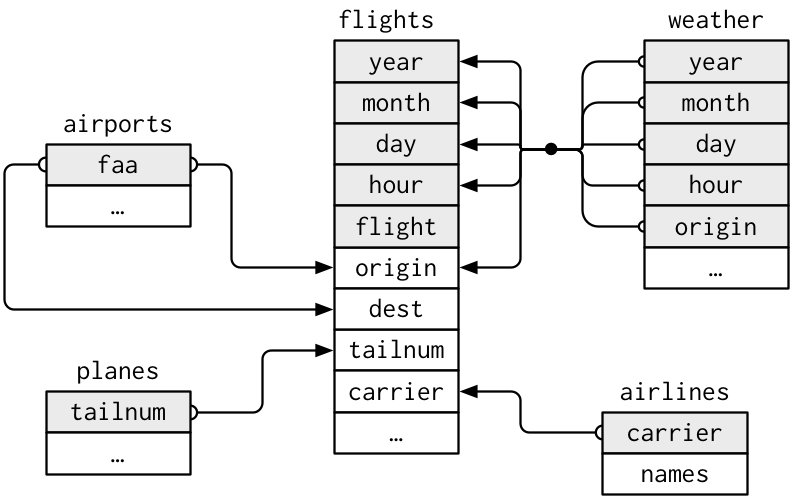
\includegraphics[width=\textwidth]{images/relational-nycflights} 

}

\caption[Data relationships in nycflights13 from R for Data Science]{Data relationships in nycflights13 from R for Data Science}\label{fig:reldiagram}
\end{figure}

\subsection{Joining by Key Variables}\label{joining-by-key-variables}

In both \texttt{flights} and \texttt{airlines}, the key variable we want
to join/merge/match the two data frames with has the same name in both
data sets: \texttt{carriers}. We make use of the \texttt{inner\_join()}
function to join by the variable \texttt{carrier}.

\begin{Shaded}
\begin{Highlighting}[]
\NormalTok{flights_joined <-}\StringTok{ }\NormalTok{flights %>%}\StringTok{ }
\StringTok{  }\KeywordTok{inner_join}\NormalTok{(airlines, }\DataTypeTok{by =} \StringTok{"carrier"}\NormalTok{)}
\KeywordTok{View}\NormalTok{(flights)}
\KeywordTok{View}\NormalTok{(flights_joined)}
\end{Highlighting}
\end{Shaded}

We observed that the \texttt{flights} and \texttt{flights\_joined} are
identical except that \texttt{flights\_joined} has an additional
variable \texttt{name} whose values were drawn from \texttt{airlines}.

A visual representation of the \texttt{inner\_join} is given below
\citep{rds2016}:

\begin{figure}

{\centering 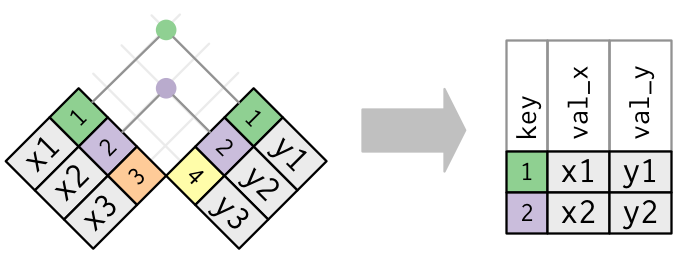
\includegraphics[width=\textwidth]{images/join-inner} 

}

\caption[Diagram of inner join from R for Data Science]{Diagram of inner join from R for Data Science}\label{fig:ijdiagram}
\end{figure}

There are more complex joins available, but the \texttt{inner\_join}
will solve nearly all of the problems you'll face in our experience.

\subsection{Joining by Key Variables with Different
Names}\label{joining-by-key-variables-with-different-names}

Say instead, you are interested in all the destinations of flights from
NYC in 2013 and ask yourself:

\begin{itemize}
\tightlist
\item
  ``What cities are these airports in?''
\item
  ``Is \texttt{"ORD"} Orlando?''
\item
  ``Where is \texttt{"FLL"}?
\end{itemize}

The \texttt{airports} data frame contains airport codes:

\begin{Shaded}
\begin{Highlighting}[]
\KeywordTok{View}\NormalTok{(airports)}
\end{Highlighting}
\end{Shaded}

However, looking at both the \texttt{airports} and \texttt{flights} and
the visual representation of the relations between the data frames in
Figure \ref{fig:ijdiagram}, we see that in:

\begin{itemize}
\tightlist
\item
  \texttt{airports} the airport code is in the variable \texttt{faa}
\item
  \texttt{flights} the airport code is in the variable \texttt{origin}
\end{itemize}

So to join these two data sets, our \texttt{inner\_join} operation
involves a \texttt{by} argument that accounts for the different names:

\begin{Shaded}
\begin{Highlighting}[]
\NormalTok{flights %>%}\StringTok{ }
\StringTok{  }\KeywordTok{inner_join}\NormalTok{(airports, }\DataTypeTok{by =} \KeywordTok{c}\NormalTok{(}\StringTok{"dest"} \NormalTok{=}\StringTok{ "faa"}\NormalTok{))}
\end{Highlighting}
\end{Shaded}

Let's construct the sequence of commands that computes the number of
flights from NYC to each destination but also includes information about
each destination airport:

\begin{Shaded}
\begin{Highlighting}[]
\NormalTok{named_dests <-}\StringTok{ }\NormalTok{flights %>%}
\StringTok{  }\KeywordTok{group_by}\NormalTok{(dest) %>%}
\StringTok{  }\KeywordTok{summarize}\NormalTok{(}\DataTypeTok{num_flights =} \KeywordTok{n}\NormalTok{()) %>%}
\StringTok{  }\KeywordTok{arrange}\NormalTok{(}\KeywordTok{desc}\NormalTok{(num_flights)) %>%}
\StringTok{  }\KeywordTok{inner_join}\NormalTok{(airports, }\DataTypeTok{by =} \KeywordTok{c}\NormalTok{(}\StringTok{"dest"} \NormalTok{=}\StringTok{ "faa"}\NormalTok{)) %>%}
\StringTok{  }\KeywordTok{rename}\NormalTok{(}\DataTypeTok{airport_name =} \NormalTok{name)}
\KeywordTok{View}\NormalTok{(named_dests)}
\end{Highlighting}
\end{Shaded}

In case you didn't know, \texttt{"ORD"} is the airport code of Chicago
O'Hare airport and \texttt{"FLL"} is the main airport in Fort
Lauderdale, Florida, which we can now see in our
\texttt{named\_freq\_dests} data frame.

\begin{center}\rule{0.5\linewidth}{\linethickness}\end{center}

\begin{learncheck}
\textbf{\emph{Learning check}}
\end{learncheck}

\textbf{(LC5.13)} Looking at Figure \ref{fig:reldiagram}, when joining
\texttt{flights} and \texttt{weather} (or, in other words, matching the
hourly weather values with each flight), why do we need to join by all
of \texttt{year}, \texttt{month}, \texttt{day}, \texttt{hour}, and
\texttt{origin}, and not just \texttt{hour}?

\textbf{(LC5.14)} What surprises you about the top 10 destinations from
NYC in 2013?

\begin{center}\rule{0.5\linewidth}{\linethickness}\end{center}

\section{Optional: Other verbs}\label{optional-other-verbs}

\subsection{Select variables using select}\label{select}

\begin{figure}

{\centering 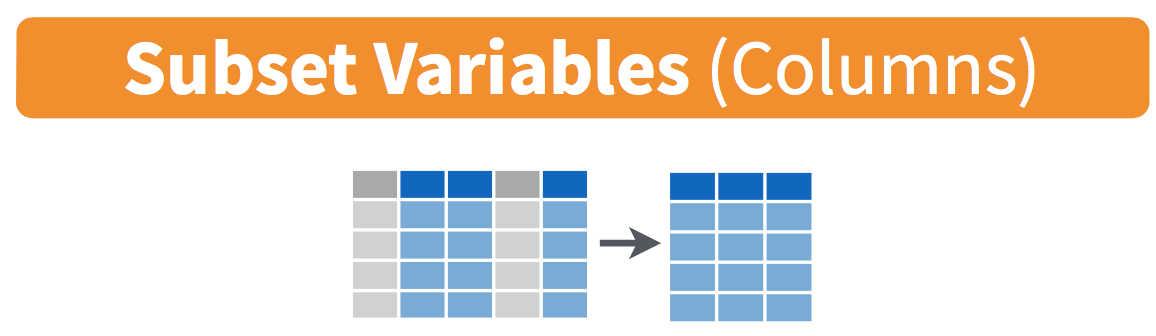
\includegraphics[width=\textwidth]{images/select} 

}

\caption[Select diagram from Data Wrangling with dplyr and tidyr cheatsheet]{Select diagram from Data Wrangling with dplyr and tidyr cheatsheet}\label{fig:selectfig}
\end{figure}

We've seen that the \texttt{flights} data frame in the
\texttt{nycflights13} package contains many different variables. The
\texttt{names} function gives a listing of all the columns in a data
frame; in our case you would run \texttt{names(flights)}. You can also
identify these variables by running the \texttt{glimpse} function in the
\texttt{dplyr} package:

\begin{Shaded}
\begin{Highlighting}[]
\KeywordTok{glimpse}\NormalTok{(flights)}
\end{Highlighting}
\end{Shaded}

However, say you only want to consider two of these variables, say
\texttt{carrier} and \texttt{flight}. You can \texttt{select} these:

\begin{Shaded}
\begin{Highlighting}[]
\NormalTok{flights %>%}\StringTok{ }
\StringTok{  }\KeywordTok{select}\NormalTok{(carrier, flight)}
\end{Highlighting}
\end{Shaded}

Another one of these variables is \texttt{year}. If you remember the
original description of the \texttt{flights} data frame (or by running
\texttt{?flights}), you'll remember that this data correspond to flights
in 2013 departing New York City. The \texttt{year} variable isn't really
a variable here in that it doesn't vary\ldots{} \texttt{flights}
actually comes from a larger data set that covers many years. We may
want to remove the \texttt{year} variable from our data set since it
won't be helpful for analysis in this case. We can deselect
\texttt{year} by using the \texttt{-} sign:

\begin{Shaded}
\begin{Highlighting}[]
\NormalTok{flights_no_year <-}\StringTok{ }\NormalTok{flights %>%}\StringTok{ }
\StringTok{  }\KeywordTok{select}\NormalTok{(-year)}
\KeywordTok{names}\NormalTok{(flights_no_year)}
\end{Highlighting}
\end{Shaded}

Or we could specify a ranges of columns:

\begin{Shaded}
\begin{Highlighting}[]
\NormalTok{flight_arr_times <-}\StringTok{ }\NormalTok{flights %>%}\StringTok{ }
\StringTok{  }\KeywordTok{select}\NormalTok{(month:day, arr_time:sched_arr_time)}
\NormalTok{flight_arr_times}
\end{Highlighting}
\end{Shaded}

The \texttt{select} function can also be used to reorder columns in
combination with the \texttt{everything} helper function. Let's suppose
we'd like the \texttt{hour}, \texttt{minute}, and \texttt{time\_hour}
variables, which appear at the end of the \texttt{flights} data set, to
actually appear immediately after the \texttt{day} variable:

\begin{Shaded}
\begin{Highlighting}[]
\NormalTok{flights_reorder <-}\StringTok{ }\NormalTok{flights %>%}\StringTok{ }
\StringTok{  }\KeywordTok{select}\NormalTok{(month:day, hour:time_hour, }\KeywordTok{everything}\NormalTok{())}
\KeywordTok{names}\NormalTok{(flights_reorder)}
\end{Highlighting}
\end{Shaded}

in this case \texttt{everything()} picks up all remaining variables.
Lastly, the helper functions \texttt{starts\_with}, \texttt{ends\_with},
and \texttt{contains} can be used to choose column names that match
those conditions:

\begin{Shaded}
\begin{Highlighting}[]
\NormalTok{flights_begin_a <-}\StringTok{ }\NormalTok{flights %>%}\StringTok{ }
\StringTok{  }\KeywordTok{select}\NormalTok{(}\KeywordTok{starts_with}\NormalTok{(}\StringTok{"a"}\NormalTok{))}
\NormalTok{flights_begin_a}
\end{Highlighting}
\end{Shaded}

\begin{Shaded}
\begin{Highlighting}[]
\NormalTok{flights_delays <-}\StringTok{ }\NormalTok{flights %>%}\StringTok{ }
\StringTok{  }\KeywordTok{select}\NormalTok{(}\KeywordTok{ends_with}\NormalTok{(}\StringTok{"delay"}\NormalTok{))}
\NormalTok{flights_delays}
\end{Highlighting}
\end{Shaded}

\begin{Shaded}
\begin{Highlighting}[]
\NormalTok{flights_time <-}\StringTok{ }\NormalTok{flights %>%}\StringTok{ }
\StringTok{  }\KeywordTok{select}\NormalTok{(}\KeywordTok{contains}\NormalTok{(}\StringTok{"time"}\NormalTok{))}
\NormalTok{flights_time}
\end{Highlighting}
\end{Shaded}

\subsection{Rename variables using rename}\label{rename}

Another useful function is \texttt{rename}, which as you may suspect
renames one column to another name. Suppose we wanted \texttt{dep\_time}
and \texttt{arr\_time} to be \texttt{departure\_time} and
\texttt{arrival\_time} instead in the \texttt{flights\_time} data frame:

\begin{Shaded}
\begin{Highlighting}[]
\NormalTok{flights_time_new <-}\StringTok{ }\NormalTok{flights %>%}\StringTok{ }
\StringTok{  }\KeywordTok{select}\NormalTok{(}\KeywordTok{contains}\NormalTok{(}\StringTok{"time"}\NormalTok{)) %>%}\StringTok{ }
\StringTok{  }\KeywordTok{rename}\NormalTok{(}\DataTypeTok{departure_time =} \NormalTok{dep_time,}
         \DataTypeTok{arrival_time =} \NormalTok{arr_time)}
\KeywordTok{names}\NormalTok{(flights_time)}
\end{Highlighting}
\end{Shaded}

It's easy to forget if the new name comes before or after the equals
sign. I usually remember this as ``New Before, Old After'' or NBOA.
You'll receive an error if you try to do it the other way:

\begin{verbatim}
Error: Unknown variables: departure_time, arrival_time.
\end{verbatim}

\subsection{Find the top number of values using
top\_n}\label{find-the-top-number-of-values-using-top_n}

We can also use the \texttt{top\_n} function which automatically tells
us the most frequent \texttt{num\_flights}. We specify the top 10
airports here:

\begin{Shaded}
\begin{Highlighting}[]
\NormalTok{named_dests %>%}\StringTok{ }
\StringTok{  }\KeywordTok{top_n}\NormalTok{(}\DataTypeTok{n =} \DecValTok{10}\NormalTok{, }\DataTypeTok{wt =} \NormalTok{num_flights)}
\end{Highlighting}
\end{Shaded}

We'll still need to arrange this by \texttt{num\_flights} though:

\begin{Shaded}
\begin{Highlighting}[]
\NormalTok{named_dests  %>%}\StringTok{ }
\StringTok{  }\KeywordTok{top_n}\NormalTok{(}\DataTypeTok{n =} \DecValTok{10}\NormalTok{, }\DataTypeTok{wt =} \NormalTok{num_flights) %>%}\StringTok{ }
\StringTok{  }\KeywordTok{arrange}\NormalTok{(}\KeywordTok{desc}\NormalTok{(num_flights))}
\end{Highlighting}
\end{Shaded}

\textbf{Note:} Remember that I didn't pull the \texttt{n} and
\texttt{wt} arguments out of thin air. They can be found by using the
\texttt{?} function on \texttt{top\_n}.

We can go one stop further and tie together the \texttt{group\_by} and
\texttt{summarize} functions we used to find the most frequent flights:

\begin{Shaded}
\begin{Highlighting}[]
\NormalTok{ten_freq_dests <-}\StringTok{ }\NormalTok{flights %>%}
\StringTok{  }\KeywordTok{group_by}\NormalTok{(dest) %>%}
\StringTok{  }\KeywordTok{summarize}\NormalTok{(}\DataTypeTok{num_flights =} \KeywordTok{n}\NormalTok{()) %>%}
\StringTok{  }\KeywordTok{top_n}\NormalTok{(}\DataTypeTok{n =} \DecValTok{10}\NormalTok{) %>%}
\StringTok{  }\KeywordTok{arrange}\NormalTok{(}\KeywordTok{desc}\NormalTok{(num_flights))}
\KeywordTok{View}\NormalTok{(ten_freq_dests)}
\end{Highlighting}
\end{Shaded}

\begin{center}\rule{0.5\linewidth}{\linethickness}\end{center}

\begin{learncheck}
\textbf{\emph{Learning check}}
\end{learncheck}

\textbf{(LC5.15)} What are some ways to select all three of the
\texttt{dest}, \texttt{air\_time}, and \texttt{distance} variables from
\texttt{flights}? Give the code showing how to do this in at least three
different ways.

\textbf{(LC5.16)} How could one use \texttt{starts\_with},
\texttt{ends\_with}, and \texttt{contains} to select columns from the
\texttt{flights} data frame? Provide three different examples in total:
one for \texttt{starts\_with}, one for \texttt{ends\_with}, and one for
\texttt{contains}.

\textbf{(LC5.17)} Why might we want to use the \texttt{select} function
on a data frame?

\textbf{(LC5.18)} Create a new data frame that shows the top 5 airports
with the largest arrival delays from NYC in 2013.

\begin{center}\rule{0.5\linewidth}{\linethickness}\end{center}

\section{Conclusion}\label{conclusion-1}

\subsection{Resources}\label{resources-1}

As we saw with the RStudio cheatsheet on
\href{https://www.rstudio.com/wp-content/uploads/2016/11/ggplot2-cheatsheet-2.1.pdf}{data
visualization}, RStudio has also created a cheatsheet for data
manipulation entitled
\href{https://github.com/rstudio/cheatsheets/raw/master/source/pdfs/data-transformation-cheatsheet.pdf}{``Data
Transformation with dplyr''}.

\subsection{Script of R code}\label{script-of-r-code-1}

An R script file of all R code used in this chapter is available
\href{http://ismayc.github.io/moderndiver-book/scripts/05-manip.R}{here}.

\begin{center}\rule{0.5\linewidth}{\linethickness}\end{center}

\begin{center}\rule{0.5\linewidth}{\linethickness}\end{center}

\begin{review}
\textbf{\emph{Review questions}}
\end{review}

Review questions have been designed using the \texttt{fivethirtyeight} R
package \citep{R-fivethirtyeight} with links to the corresponding
FiveThirtyEight.com articles in our free DataCamp course
\textbf{Effective Data Storytelling using the \texttt{tidyverse}}. The
material in this chapter is covered in the chapters of the DataCamp
course available below:

\begin{itemize}
\item
  \href{https://campus.datacamp.com/courses/effective-data-storytelling-using-the-tidyverse/filtering-grouping-summarizing}{Filtering,
  Grouping, \& Summarizing}
\item
  \href{https://campus.datacamp.com/courses/effective-data-storytelling-using-the-tidyverse/dplyr-review-8?ex=1}{dplyr
  Review}
\end{itemize}

\begin{center}\rule{0.5\linewidth}{\linethickness}\end{center}

\begin{center}\rule{0.5\linewidth}{\linethickness}\end{center}

\subsection{What's to come?}\label{whats-to-come-2}

This concludes the \textbf{Data Exploration} unit of this book. You
should be pretty proficient in both plotting variables (or multiple
variables together) in various data sets and manipulating data as we've
done in this chapter. You are encouraged to step back through the code
in earlier chapters and make changes as you see fit based on your
updated knowledge.

In Chapter \ref{sim}, we'll begin to build the pieces needed to
understand how this unit of \textbf{Data Exploration} can tie into
statistical inference in the \textbf{Inference} part of the book.
Remember that the focus throughout is on data visualization and we'll
see that next when we discuss sampling, resampling, and bootstrapping.
These ideas will lead us into hypothesis testing and confidence
intervals.

\renewcommand{\bibname}{References}
\addcontentsline{toc}{chapter}{References}
\bibliography{bib/packages.bib,bib/books.bib,bib/articles.bib}
% 
% 

\end{document}
